\documentclass[a4paper]{article} 
\addtolength{\hoffset}{-2.25cm}
\addtolength{\textwidth}{4.5cm}
\addtolength{\voffset}{-3.25cm}
\addtolength{\textheight}{5cm}
\setlength{\parskip}{0pt}
\setlength{\parindent}{0in}

\usepackage{blindtext} % Package to generate dummy text
\usepackage{charter} % Use the Charter font
\usepackage[utf8]{inputenc} % Use UTF-8 encoding
\usepackage{microtype} % Slightly tweak font spacing for aesthetics
\usepackage[english]{babel} % Language hyphenation and typographical rules
\usepackage{amsthm, amsmath, amssymb, amsfonts, nccmath} % Mathematical typesetting
\usepackage{float} % Improved interface for floating objects
\usepackage[final, colorlinks = true, 
linkcolor = black, 
citecolor = black]{hyperref} % For hyperlinks in the PDF
\usepackage{graphicx, multicol} % Enhanced support for graphics
\usepackage{xcolor} % Driver-independent color extensions
\usepackage{marvosym, wasysym} % More symbols
\usepackage{rotating} % Rotation tools
\usepackage{subcaption}
\usepackage{wrapfig}
% \usepackage{geometry}
\usepackage{censor} % Facilities for controlling restricted text
\newcommand{\note}[1]{\marginpar{\scriptsize \textcolor{red}{#1}}} % Enables comments in red on margin
\usepackage{bm}
\usepackage{blkarray}
\usepackage{enumitem}
\usepackage{pgfplots}
\usepackage{tikz}
\usetikzlibrary{bayesnet}

\usepackage{tcolorbox}
\usepackage[ruled,vlined]{algorithm2e}

\newcommand{\pd}[2]{\frac{\partial #1}{\partial #2}}
\newcommand{\loss}[0]{\mathcal{L}}
\newcommand{\chain}[3]{\frac{\partial #1}{\partial #2}\frac{\partial #2}{\partial #3}}
% \newcommand{\eq}[1]{\begin{equation*}\begin{split}#1\end{split}\end{equation*}}
\newcommand{\TODO}[1]{\textbf{\textcolor{red}{#1}}}
\newcommand{\E}[0]{\mathbb{E}} % Expectation
\newcommand{\R}[0]{\mathbb{R}} % Real numbers
\newcommand{\Cdo}[0]{\textnormal{do}}
\newcommand{\Prob}[1]{\Pr\left\{#1\right\}} % Real numbers
\newcommand\independent{\protect\mathpalette{\protect\independenT}{\perp}}
\def\independenT#1#2{\mathrel{\rlap{$#1#2$}\mkern2mu{#1#2}}}
\newcommand*{\QED}{\hfill\ensuremath{\blacksquare}}%

\definecolor{green}{RGB}{0,160,0}
\definecolor{blue}{RGB}{0,0,160}
\definecolor{red}{RGB}{160,0,0}
\definecolor{orange}{RGB}{200,160,0}
\definecolor{purple}{RGB}{170,0,200}
\definecolor{cyan}{RGB}{0,200,200}
\definecolor{lightred}{RGB}{200,50,50}

\setcounter{tocdepth}{2}
% Title Page
\title{Summary Reinforcement Learning}
\author{Phillip Lippe}


\begin{document}
\maketitle
\tableofcontents
\newpage

\section{Introduction to Reinforcement Learning}
\textit{This section reviews the lecture slides 1 and 2 (until Monte Carlo). }
\begin{itemize}
	\item Reinforcement Learning deals with the following question: 
	
	How to \textcolor{blue}{sequentially interact} with an environment to \textcolor{blue}{maximize a long-term objective}?
	
	\item The general RL setting is visualized in Figure~\ref{fig:rl_introduction_reinforcement_learning}. Thereby we have 4 variables that are passed around:
	\begin{itemize}
		\item The state $S_t$, in which the agent currently is, determined by the environment
		\item The action $A_t$ which is chosen by the agent, based on the observation of the state $S_t$
		\item Based on the interaction $A_t$, the agent ends up in a new state $S_{t+1}$ as well as getting a reward $R_{t+1}$. Both properties are determined by the environment, and can only be influenced by the agent through $A_t$
	\end{itemize}
	\begin{figure}[ht!]
		\centering
		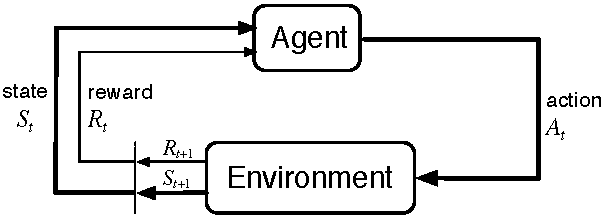
\includegraphics[width=0.4\textwidth]{figures/rl_introduction_reinforcement_learning.pdf}
		\caption{Illustration of the interaction of an agent with an environment in the reinforcement learning setting.}
		\label{fig:rl_introduction_reinforcement_learning}
	\end{figure}

	\item The decision of which action to take at which state is called policy, and we denote it by $\pi$. The goal is to find the optimal policy $\pi$ which maximizes the reward we get from the environment
		
	\item As we learn by interactions, we have major main challenges in contrast to standard supervised learning:
	\begin{itemize}
		\item The dataset is not static as in e.g. image classification. Every time we change our policy, new data has to be generated as the actions we take at certain states are different. Note that there are techniques to use the data more efficiently, and we will discuss them later.  
		\item Instead of having i.i.d. data, we have sequential data which are highly correlated. Standard optimizers like SGD fail because they assume i.i.d. inside a batch. We will also discuss how we can tackle this problem.
	\end{itemize}
\end{itemize}
\subsection{MDPs and $k$-armed bandits}
\begin{itemize}
	\item A common used, simplified example for RL is a $k$-armed bandit. We can image it as $k$ slot machines with unknown pay-off distribution. Hence, we have a static environment where the mapping function between actions and rewards is independent of state and time step $t$
	\item Our goal is to maximize the cumulative reward over time. There are two variants we can use:
	\begin{itemize}
		\item If we want to maximize our reward for a finite horizon $T$ (i.e. limited number of trials), our goal is to maximize $\sum_{t=1}^{T} r_t$
		\item If we assume that we can take as many actions as we want, we have the objective for infinite horizon: $\sum_{t=1}^{\infty} \gamma^{t}r_t$ where $\gamma\in [0,1]$ is a discount factor. Note that if we would not have a discount factor, we end up with infinite reward for any action whose reward has a mean greater than zero.
		\item For generalization, we call $G_t=\sum_{k=0}^{\infty} \gamma^{k}R_{t+k+1}=R_{t+1}+\gamma G_{t+1}$ the \textbf{(discounted) return}, or cumulative reward, at time step $t$. Only if a episode terminates (meaning that we cannot play forever), a discount factor of $\gamma=1$ is allowed.
	\end{itemize} 
	\item A general trade-off in reinforcement learning is between \textbf{exploration} (i.e. trying new actions) and \textbf{exploitation} (i.e. taking best actions we know). If we perform too little exploration, we might overlook the best action, for example due to stochasticity of the reward. However, exploiting the best actions is likely to lead to the maximum rewards, so that with exploring, we ``loose'' possible rewards.
	
	A general rule of thumb is: if we have much time left or are very uncertain about our current estimates, do more exploration. If we are limited on time, or are certain about our estimates, we should exploit more. 
	
	Also $\gamma$ can play a role as the higher $\gamma$, the more we care about rewards in the future, and hence, should perform more exploration.
	
	\item We now introduce a set of important functions which are used for finding the optimal policy:
	\begin{itemize}
		\item The \textbf{state-action value function}, also called \underline{$q$-function}, expresses the expected return of taking a certain action in a given state:
		$$q_{\pi}(s,a)=\E_{\pi}[G_t|S_t=s,A_t=a]$$
		Note that $q$-value is always specific to a certain policy as $G_t$ is in expectation that all steps after $t$ are taken according to the policy $\pi$
		\item The \textbf{state-value function} is similar to the $q$ function, but only takes the state into account, and considers the action under the expectation:
		$$v_{^\pi}(s)=\E_{\pi}[G_t|S_t=s]$$
	\end{itemize}

	\item In the case of the k-armed bandit, we try to learn a $q$-function (as we want to find the best action) but assume that we stay in the same state $s$. To balance exploration and exploitation, there are different strategies possible, for example:
	\begin{itemize}
		\item \textbf{$\epsilon$-greedy} takes in $(1-\epsilon)$ cases the optimal action, and with the chance of $\epsilon$ selects an action randomly
		\item An annealed softmax takes the estimated action value into account, and creates a distriubtion based on this with a temperature factor $\tau$ (high $\tau$ means more stochasticity):
		$$p(a)=\frac{\exp\left(\hat{q}(a)/\tau\right)}{\sum_{a'}\exp\left(\hat{q}(a')/\tau\right)}$$
		\item We can use the current estimate $\hat{q}$ in combination with the uncertainty we have a certain action. This leads to the Upper confidence bound, or we can alternatively initialize all $q$-values optimistically (guarantees certain level of exploration)
	\end{itemize} 

	\item \textbf{Markov Decision Process}: An agent chooses an action which only depends on the current state $s_t$, and is independent of the history $s_0,...,s_{t-1}$ given $s_t$. Formally, we can define a finite MDP by
	\begin{itemize}
		\item A finite set of states $\mathcal{S}$
		\item A finite set of actions for each state $\mathcal{A}_s$ (often the same in all states)
		\item A dynamics function $p(s',r|s,a)=\Prob{S_t=s',R_t=r|S_{t-1}=s,A_{t-1}=a}$ which is often split into
		\begin{itemize}
			\item Transition function $p(s'|s,a)$
			\item Reward function $p(r|s,a,s')$
		\end{itemize}
		\item A discount factor $\gamma\in[0,1]$
	\end{itemize}
	\item In this setting, the optimal action can be found by optimizing the policy $\pi^{*}(s_t)$. In the rest of the course, we mostly focus on MDPs
\end{itemize}

\subsection{Dynamic Programming}
\begin{itemize}
	\item For simple environments where we know the dynamics function of the MDP, we can apply approaches of dynamic programming
	\item One thing to notice about the functions $v$ and $q$ are their relationships, namely:
	\begin{equation*}
		\begin{split}
			v(s) & = \E_{\pi}\left[G_t|S_t=s\right] = \E_{a\sim\pi}\left[\E_{\pi}\left[G_t|S_t=s,A_t=a\right]\right] = \E_{a\sim\pi} q_{\pi}(s,a)\\[8pt]
			q(s,a) & = \E_{\pi}[G_t|S_t=s,A_t=a] = \E_{\pi}[R_{t+1}|S_t=s,A_t=a]+\E_{s',\pi}[\gamma G_{t+1}|S_{t+1}=s'] \\& = \E_{s',\pi}[R_{t+1}+\gamma v(s')|S_t=s,A_t=a,S_{t+1}=s']
		\end{split}
	\end{equation*}
	\item A policy is optimal if there is no other policy for which the value of any state is larger than the current one: $v_{*}(s)=\max_{\pi} v_{\pi}(s)$, $q_{*}(s,a)=\max_{\pi} q_{\pi}(s,a)$
	\item Again, we can write down the relations between the two functions, which are called \textit{Bellman optimality equations} for the optimal case:
	\begin{equation*}
		\begin{split}
			v_{*}(s) & =\max_{a}q_{*}(s,a)= \max_a \E\left[R_{t+1}+\gamma v_{*}(S_{t+1})|S_t=s,A_t=a\right]\\
			q_{*}(s,a) & = \max_{a}\E\left[R_{t+1}+\gamma \max_{a'} q_{*}(S_{t+1},a')|S_t=s,A_t=a\right]
		\end{split}
	\end{equation*}
	
	\item The first approach of finding the optimal policy is \textbf{policy iteration}. It combines two steps:
	\begin{itemize}
		\item \textit{Policy evaluation}: given a policy $\pi$, we try to find the corresponding value function $v_{\pi}$. We do this by performing the update $v(s)=\E[R_{t+1}+\gamma v(s)]$ until the values converge. Note that we can evaluate the expectation as we know $\pi$ and the MDP dynamics $p(s',r|s,a)$
		\item \textit{Policy improvement}: given the value function $v_{\pi}$, we try to find a new policy for which we know that $\forall s, v_{\pi'}(s)\geq v_{\pi}(s)$. We can do that by taking the argmax over actions in each state.
	\end{itemize}
	Policy iteration performs these two in a loop until the policy is not changed anymore in the improvement step. It is guaranteed to converge to the optimal policy $\pi$.
	
	The full algorithm is shown in Figure~\ref{fig:rl_introduction_policy_iteration}.
	\begin{figure}[ht!]
		\centering
		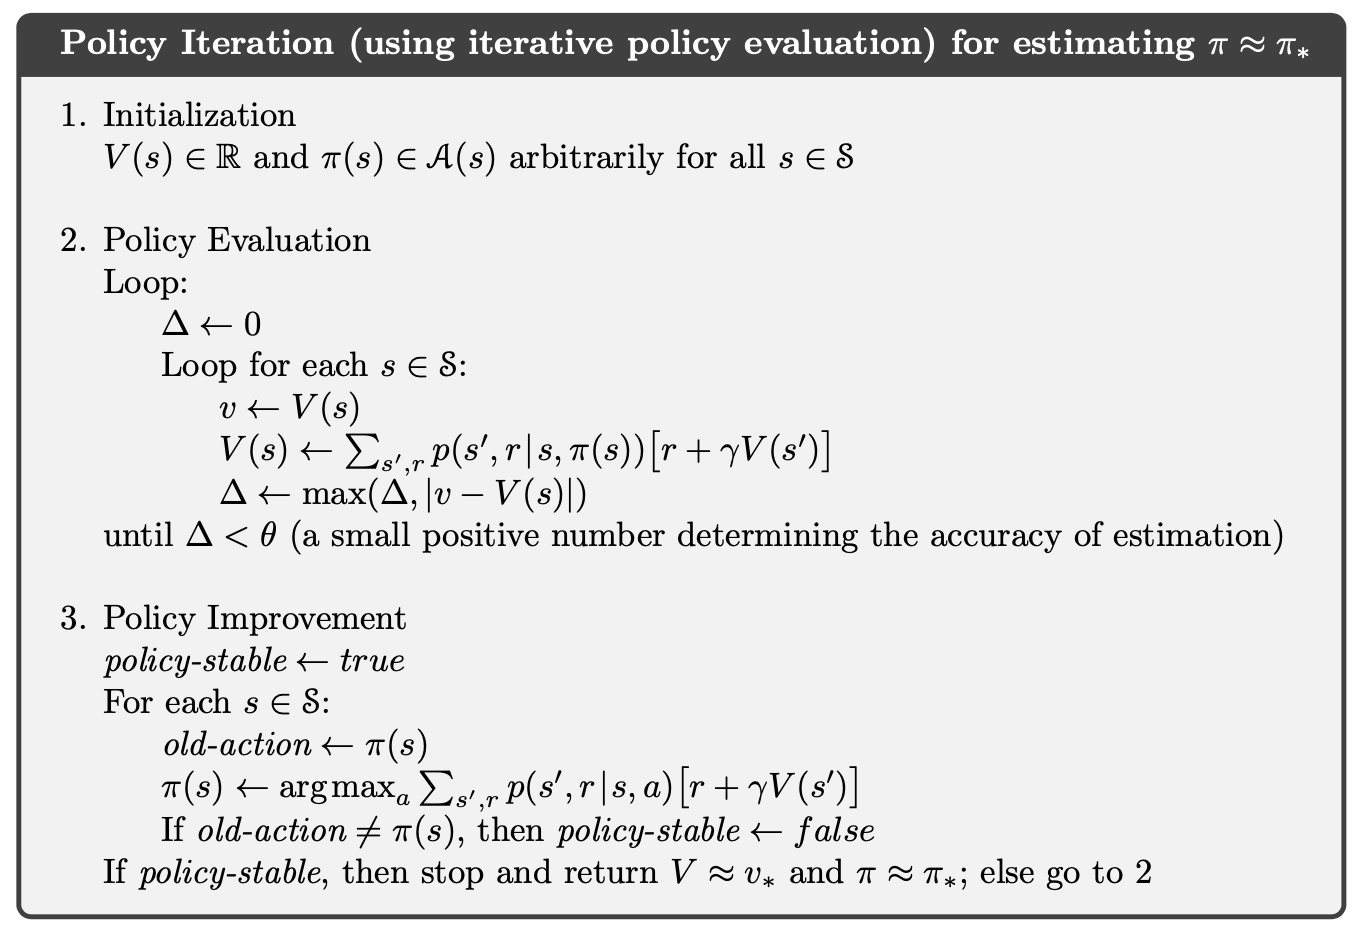
\includegraphics[width=0.7\textwidth]{figures/rl_introduction_policy_iteration.png}
		\caption{Policy iteration algorithm (Sutton book)}
		\label{fig:rl_introduction_policy_iteration}
	\end{figure}
	\item The issue of policy iteration is that the policy evaluation step can take a long time until it fully converges, although slight changes might not influence the policy too much. An alternative is to stop policy evaluation after a single iteration, and directly optimize it. This leads to the \textbf{value iteration algorithm}.
	
	When implementing it, we can efficiently combine the two steps of evaluation and improvement, which is actually the same as performing the Bellman optimality equation as an update step. See Figure~\ref{fig:rl_introduction_value_iteration} for details.
	
	\begin{figure}[ht!]
		\centering
		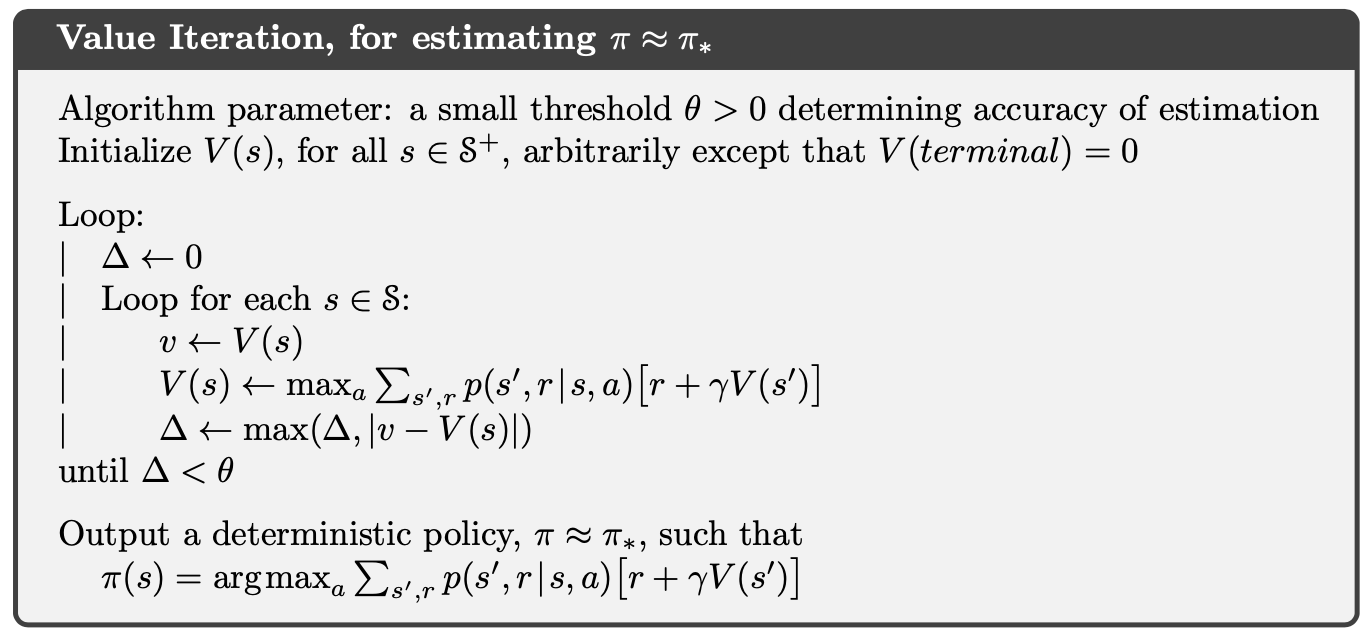
\includegraphics[width=0.7\textwidth]{figures/rl_introduction_value_iteration.png}
		\caption{Value iteration algorithm (Sutton book)}
		\label{fig:rl_introduction_value_iteration}
	\end{figure}

	The drawback of value iteration is that it can lead to noisy updates as it only performs a single update step and hence, can give inaccurate estimates of $v$. In practice, what has been found to mostly work the best, is to perform a limited, small number of steps of policy evaluation.
	
	\item Keep in mind that for all these algorithms we require to know the MDP dynamics $p(s',r|s,a)$. However, this is often not the case, especially for more complicated, real-world environments. There we can only sample data point $(s_i,a_i,r_i,s'_i)$ which we need to use effectively. 
	
\end{itemize}
\subsection{Outline}
\begin{itemize}
	\item In the next sections (and rest of the whole course), we will deal with different ways of learning the optimal policy when the dynamics of the MDP are unknown in advance. We can distinguish the approaches into three main groups (see Figure~\ref{fig:rl_introduction_overview_leanring_techniques}):
	\begin{itemize}
		\item \textbf{Value-based} methods try to learn the value functions $v(s)$ and $q(s,a)$ from interactions with the environment. Based on these, we can find the optimal policy $\pi$.
		\item \textbf{Policy-based} methods try to directly learn the desired objective, namely the policy $\pi$. While we prevent propagating errors to the policy from learning a value function, it is often harder to optimize.
		\item In contrast to the previous techniques, \textbf{model-based} RL is based on the idea of learning the dynamics of the MDP, namely $p(s',r|s,a)$. With this knowledge given, we can then again apply value-based or policy-based methods, but support them by either using the transition function directly (i.e. take all possible future states into account instead of sampling), or simulate new trajectories if this is expensive in the original environment. 
	\end{itemize}
	\begin{figure}[ht!]
		\centering
		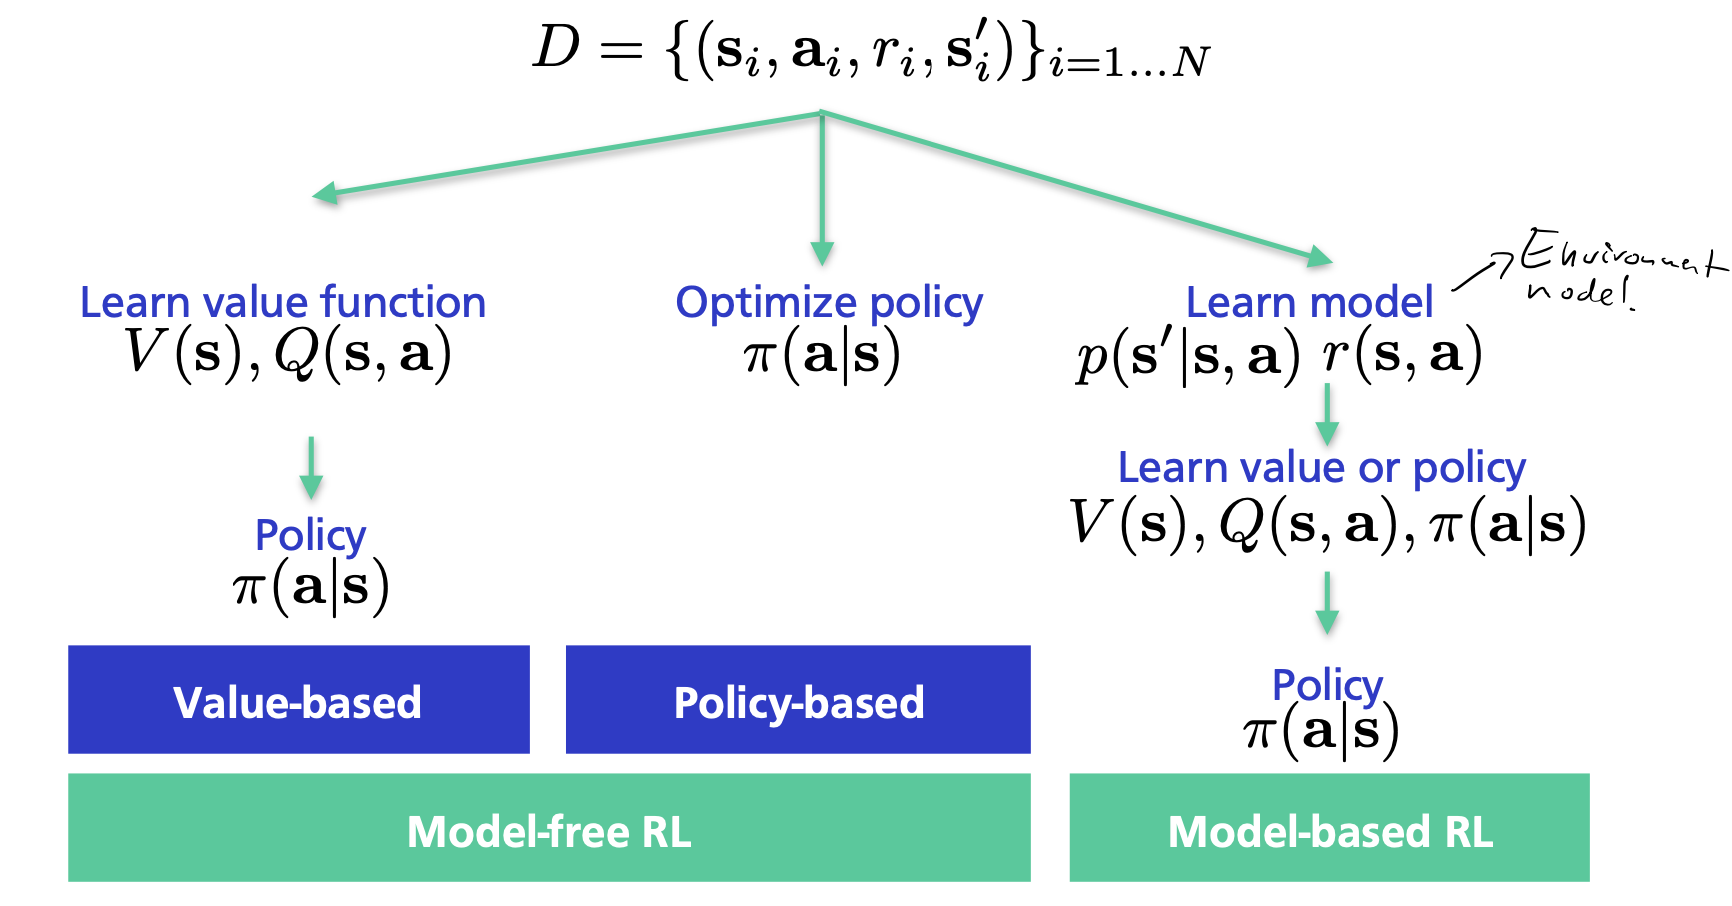
\includegraphics[width=0.5\textwidth]{figures/rl_introduction_overview_leanring_techniques.png}
		\caption{Overview of different learning strategies in RL.}
		\label{fig:rl_introduction_overview_leanring_techniques}
	\end{figure}
	\item The next sections 2 and 3 (lecture slides 3 to 6) deal with value-based methods. First, we discuss tabular-based techniques, meaning that we store e.g. $v(s)$ by a big table (i.e. every state has an entry in this table). However, these methods cannot be applied if the state space is continuous and/or high-dimensional (size increases exponentially). Thus, we look at approximations in section 3.
	\item Section 4 (lecture slides 7 to 10) deals with policy-based RL introducing different techniques for approximating the optimal gradients in policy learning.
	\item Model-based RL is discussed in section 5 (lecture slides 11 and 12), but in less details than the previous two.
	\item The final chapter deals with partially-observable environments (Section 7, lecture 13), and how to take uncertainty into account.
\end{itemize}
\newpage
\section{Value-based RL: Tabular Methods}
\textit{This section reviews the lecture slides 2 (Monte Carlo), 3 and 4.}
\subsection{Monte Carlo}
\begin{itemize}
	\item We can try to estimate the value function by simply sampling from the expectation, meaning we generate episodes, and evaluate the cumulative reward:
	$$v(s_t)=\E_{\pi}\left[\sum_{k=0}^{\infty} \gamma^k R_{t+k+1}\Big\vert S_t=s\right]\approx \frac{1}{N}\sum_{n=1}^{N}\sum_{k=0}^{T_{n}}\gamma^k R_{t+k+1}^{(n)}$$
	Note that this requires the task to be \textbf{episodic}, meaning that an episode always ends. Otherwise, we are not able to sample 
	\item We can get into the situation that we visit the same state twice in a trajectory. In the update, we can either just take the first time into account that we visited $s$ (\textit{first-visit MC}), or we can consider all of them as different points (\textit{every-visit MC}). Both approaches are very similar, and converge to the same optimum. However, every-visit MC leads to slightly biased estimates if number of samples is low.
	\item If we want to use Monte-Carlo for learning the optimal policy, we need to slightly adjust our algorithm. First, note that we rather want to learn the $q$-value as we can determine the optimal policy from them by greedifying: $\pi_{*}(s)=\arg\max_a q_{*}(s,a)$
	\item To guarantee that every state-action pair is visited, we can either:
	\begin{itemize}
		\item Perform ``exploring starts'', meaning that we randomly sample our start state $(S_0,A_0)$. However, note that this requires an environment where we can set the agent to any position, which is not always possible (e.g. in physical systems, hard to initialize velocity or acceleration)
		\item Use policy that visits every state and actions with non-zero probability. 
	\end{itemize}
	\item As the random starts are often not possible, we mostly choose to integrate exploration into our policy. We can either do this by updating our policy \textit{towards} the greedy one, but not match it exactly (called \textbf{on-policy}). Or we sample from a non-greedy behavior policy but update with respect to our greedy one (called \textbf{off-policy}).
\end{itemize}
\subsubsection{On-policy MC}
\begin{itemize}
	\item To ensure that every action is taken with a non-zero probability, we can use policies like $\epsilon$-greedy. Every time we update our $q$-value, we can update our policy by making it greedy on $q$, and adding $\epsilon$ as probability for choosing a random action.
	\item We can show that choosing our $\epsilon$-greedy policy by that actually leads to the optimal $\epsilon$-greedy policy, as:
	\begin{equation*}
		\begin{split}
			q_{\pi}(s,\pi'(s)) & =\frac{\epsilon}{|\mathcal{A}(s)|}\sum_a q_{\pi}(s,a) + \left(1-\epsilon\right)\max_a q_{\pi}(s,a)\\
			v_{\pi}(s) & = \frac{\epsilon}{|\mathcal{A}(s)|} \sum_a q_{\pi}(s,a) + (1-\epsilon)\left[\sum_{a}\frac{\pi(a|s)-\frac{\epsilon}{|\mathcal{A}(s)|}}{1-\epsilon} q_{\pi}(s,a)\right]\\
		\end{split}
	\end{equation*}
	To show that we improve, we need to show that $v_{\pi'}(s)\geq v_{\pi}(s)$. As the stochastic part $\frac{\epsilon}{|\mathcal{A}(s)|} \sum_a q_{\pi}(s,a)$ is unaffected by $\pi$, we only have to compare the greedy part:
	\begin{equation*}
		\begin{split}
			\sum_{a}\frac{\pi'(a|s)-\frac{\epsilon}{|\mathcal{A}(s)|}}{1-\epsilon} q_{\pi}(s,a) \geq \sum_{a}\frac{\pi(a|s)-\frac{\epsilon}{|\mathcal{A}(s)|}}{1-\epsilon} q_{\pi}(s,a)\\
		\end{split}
	\end{equation*}
	where we can put in $\pi'$ as the greedy policy:
	\begin{equation*}
		\begin{split}
			\max_a q_{\pi}(s,a) \geq \sum_{a}\frac{\pi(a|s)-\frac{\epsilon}{|\mathcal{A}(s)|}}{1-\epsilon} q_{\pi}(s,a)
		\end{split}
	\end{equation*}
	This is obviously true because there is no actions besides the greedy one which gives higher reward. 
	\item Hence, when we updating the policy, we either improve or stay equally optimal. Note that this only holds for $\epsilon$-soft policies, meaning policies for which every action has at least $\epsilon/|\mathcal{A}(s)|$ probability of being selected
\end{itemize}
\subsubsection{Off-policy MC}
\begin{itemize}
	\item In off-policy, we have a behavior policy $b$ from which we sample the trajectories, and our greedy target policy $\pi$. The only constraint on $b$ is that for any action where $\pi(a|s)>0$, $b$ also needs to be $b(a|s)>0$. We can ensure this by any $\epsilon$-soft policy
	\item When sampling, we need to correct for the fact that we use samples from $b$ to evaluate an expectation over $\pi$. One way of doing so is importance sampling:
	$$v_{\pi}(s) \approx \frac{1}{N}\sum_{n=1}^{N} \frac{p(\tau^{n}_{t}|s,A_t\sim\pi)}{p(\tau^{n}_{t}|s,A_t\sim b)} G(\tau_{t}^{n})$$
	where $\tau^{n}_{t}$ is the $n$-th trajectory starting from time step $t$ till the end. We can rewrite the importance weights as $\rho_{t:T-1}=\frac{\prod_{k=t}^{T-1}\pi(A_k|S_k)}{\prod_{k=t}^{T-1}b(A_k|S_k)}$. Note that the transition probabilities between $S_{t}$ and $S_{t+1}$ cancel out as they are the same for $\pi$ and $b$.
	\item When using these importance weight, there are two ways we can average over them:
	\begin{itemize}
		\item \textbf{Ordinary} importance sampling averages by taking the number of trajectories into account:
		$$v_{\pi}(s)=\frac{\sum_{t\in\mathcal{T}(s)}\rho_{t:T(t)-1}G_t}{|\mathcal{T}(s)|}$$
		While this gives us an unbiased estimate, also for small sample sizes, it suffers from high variance when $\rho_{t:T(t)-1}$ varies a lot (e.g. $b$ and $\pi$ quite different)
		\item \textbf{Weighted} importance sampling averages by summing over weights:
		$$v_{\pi}(s)=\frac{\sum_{t\in\mathcal{T}(s)}\rho_{t:T(t)-1}G_t}{\sum_{t\in\mathcal{T}(s)}\rho_{t:T(t)-1}}$$
		This approach reduces the variance because we take into account whether we mostly have big or small values of $\rho_{t:T(t)-1}$, but gives an biased estimate. Suppose we have a single sample, then the importance weight cancels out, meaning we estimate $v_{\pi}(s)\approx v_{b}(s)$. The more samples we get, the lower this bias gets.
	\end{itemize}
	Note that while both give the same correct result for $N\to\infty$, they differ for cases with limited sample size. In practice, the lower variance is mostly preferred so that weighted importance sampling is usually applied.
	\item For implementing this, we take an incremental approach as we can calculate importance weights by $\rho_{t:T(t)-1}=\frac{\pi(A_t|S_t)}{b(A_t|S_t)}\rho_{t+1:T(t)-1}$ which we denote by $W$ in Figure~\ref{fig:rl_tabular_methods_offpolicy_MC_control}. Hence, given a trajectory, we should start with the last state, and iterate to the start state.
	
	\begin{figure}[ht!]
		\centering
		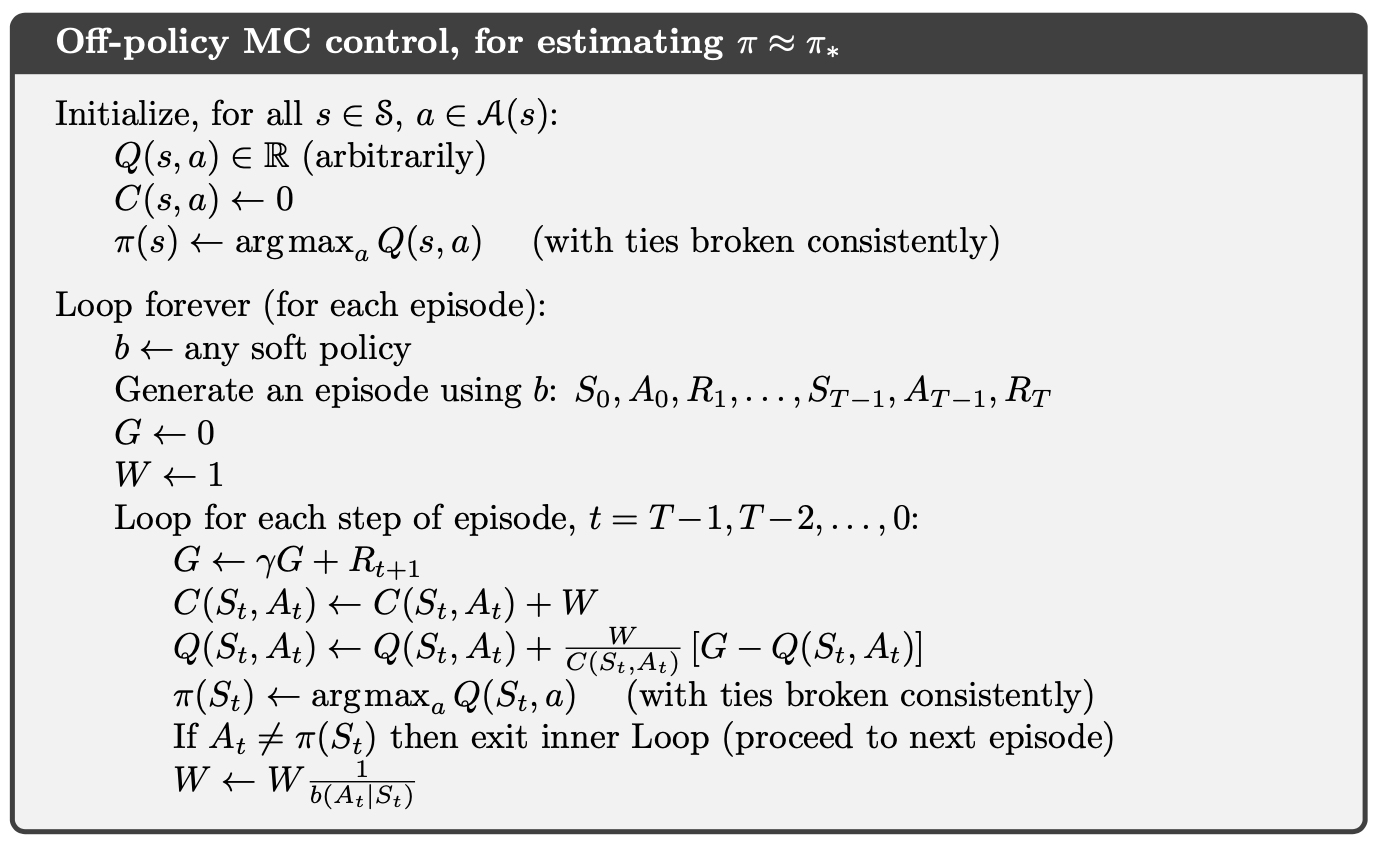
\includegraphics[width=0.6\textwidth]{figures/rl_tabular_methods_offpolicy_MC_control.png}
		\caption{Incremental implementation of Off-policy Monte-Carlo control.}
		\label{fig:rl_tabular_methods_offpolicy_MC_control}
	\end{figure}
	
	Furthermore, to perform the averaging efficiently, we need to keep track of the normalization constant which is the sum of all importance weights for a certain state-action pair. This we will store in $C$. 
	
	In case we use a greedy policy for $\pi$, we can simplify the algorithm further. In the importance weight, $\pi(A_t|S_t)$ is 1 if $A_t$ was the greedy action, otherwise, we have a factor of 0 (which gives $\rho=0$ for all previous actions). If we update our states in a reverse manner, this means that we can stop the loop as soon as we hit a sub-optimal action. 
	
	Note that $W$ can get fairly large for long trajectories, as $b(A|S)$ is always smaller than 1. We need to use weighted importance sampling instead of ordinary as otherwise, the variance is too high. In addition, as only the tails of the episode are updated frequently, we might have an insufficient amount of samples for the states close to the start, which makes the algorithm inefficient.
	
	
\end{itemize}
\subsubsection{On-policy versus Off-policy control}
\label{sec:value_based_tabular_on_off_policy}
\begin{itemize}
	\item After reviewing two alternative ways of learning a policy for a given environment, we can consider what are the advantages and drawbacks of each of the methods
	\item In general, we can note that off-policy is actually a generalization of on-policy because if we set the behavior policy equal to our target policy, i.e. $b=\pi$, then off-policy becomes on-policy
	\item Commonly, on-policy converges faster as it uses the samples from the same policy it updates for. Off-policy can introduce variance by correcting the estimates for the target policy, as e.g. the importance weight can vary a lot if $\pi$ and $b$ are quite different. This can lead to slow convergence.
	\item A benefit of off-policy is however that we can learn from already recorded data, eventually from another source, as only our updates are based on the current policy $\pi$, and not the actual samples as in on-policy. This means that we could use the same data to evaluate multiple policies, which especially helps for limited data/interactions with the environment.
	\item Another point to consider is that off-policy methods allow us to learn the actual greedy policy. This is not possible in the on-policy setting because for guaranteeing the convergence to the correct $q$-values, we need to give every state-action pair a chance greater than zero to be visited. Using an $\epsilon$-soft policy in the on-policy method and greedifying it afterwards can lead to a good approximation, but we also need to keep in mind that we then learn the optimal $\epsilon$-soft policy, and not the strictly the optimal greedy policy. Hence, our final moves might be sub-optimal (remember Cliff-World, Sutton Book Example 6.6, page 132)
\end{itemize}

\subsection{Temporal-Difference Learning}
\begin{itemize}
	\item Combining the ideas of Monte Carlo and Dynamic Programming, we arrive at a different type of methods, called Temporal difference learning. Remember that we can define the value function as a recursive function: $v(s)=\E[R_{t+1}+\gamma v(S_{t+1})|S_t=s]$. We can use this equality as a target instead of $G_t$, leading to the following update rule:
	$$v(s_t)\leftarrow v(s_t)+\alpha\underbrace{\left[R_{t+1}+\gamma v(s_{t+1}) - v(s_t)\right]}_{\text{TD error } \delta_t}$$
	Instead of waiting for a full episode to finish, we can perform this update after \textit{a single action} taken in the environment. This method is called TD(0), and we will see later that this is a special case of TD($\lambda$), or $n$-step TD
	\item TD(0) is a \textit{bootstrapping} method as it uses its own estimates as targets. 
	\item There are two main approaches for learning policies with Temporal Difference, namely \textbf{SARSA} and \textbf{Q-learning}, which we will now discuss in detail. Both learn the $q$-function, but have slightly different update rules.
	
	Note that TD learning can of course also be used for policy evaluation by simply performing the update rule above on samples from the original policy until our value function converges
\end{itemize}
\subsubsection{SARSA}
\begin{itemize}
	\item The update rule of SARSA is as follows:
	$$Q(S_t,A_t)\leftarrow Q(S_t,A_t) + \alpha\left[R_{t+1}+\gamma Q(S_{t+1},A_{t+1})-Q(S_t,A_t)\right]$$
	where $A_{t+1}$ is selected by the policy $\pi$ based on $S_{t+1}$. Note that $Q(S_{t+1},A_{t+1})=0$ for the terminal state.
	\item The method got its name from using $\bm{S}_t$, $\bm{A}_t$, $\bm{R}_{t+1}$, $\bm{S}_{t+1}$, $\bm{A}_{t+1}$ in its update rule.
	\item Note that SARSA is a \textbf{on-policy} method, meaning that it learns the $q$-values of the policy $\pi$ (see Section~\ref{sec:value_based_tabular_on_off_policy} for discussion of benefits and drawbacks)
	\item Instead of just using the next sample to estimate $Q(S_{t+1},A_{t+1})$, we could also take our policy into account as we can calculate the expectation operator over it instead of simply sampling:
	\begin{equation*}
		\begin{split}
			Q(S_t,A_t) & \leftarrow Q(S_t,A_t) + \alpha\left[R_{t+1}+\gamma \E_{\pi}[Q(S_{t+1},A_{t+1})|S_{t+1}]-Q(S_t,A_t)\right]\\
			& \leftarrow Q(S_t,A_t) + \alpha\left[R_{t+1}+\gamma \sum_{a} \pi(a|S_{t+1}) Q(S_{t+1},a)-Q(S_t,A_t)\right]
		\end{split}
	\end{equation*}
	This method is also called \textbf{expected SARSA}
	\item Note that we can perform \textbf{off-policy} control with expected SARSA, where we use a different behavior policy $b$ to sample, but learn the $q$-values of $\pi$. A special case of this is when we choose $\pi$ to be the greedy policy, which leads to the \textbf{Q-learning algorithm}
\end{itemize}

\subsubsection{Q-Learning}
\begin{itemize}
	\item As mentioned before, Q-learning applies a greedy policy in expected SARSA. This simplifies the update rule to:
	$$Q(S_t,A_t)\leftarrow Q(S_t,A_t) + \alpha\left[R_{t+1}+\gamma \max_a  Q(S_{t+1},a)-Q(S_t,A_t)\right]$$
	\item It can be shown that Q-learning converges to the optimal $q_{*}$ under the condition, that the learning rate $\alpha$ goes to zero (but not too fast), and every state-action pair is visited infinite amount of times when we have infinite number of steps.
	\item However, there are also disadvantages of using the greedy policy. Suppose you have multiple actions with the same value $q(s,a)=0$ as ground truth. When learning it, we will have a certain amount of noise on it, so that some are slightly lower and other slightly above 0. When we now take the maximum, $\max_a q(s,a)$, we get a positive value although the GT is zero. Hence, we have a positive bias, to which we also refer to as \textbf{maximization bias}.
	\item This bias can occur when we use a maximum operator in our update step. Hence, it is also the case for SARSA if it uses a $\epsilon$-greedy policy
	\item With infinite number of samples it might become less relevant, but we are usually limited in computational resources/time. Take for example the environment in Figure~\ref{fig:rl_tabular_methods_maximization_bias}. The action of going left has a obviously lower expected reward, but due to the maximization bias, we will have for some actions from $B$ positive rewards (due to a high variance), and hence, we prefer going left. If we limit our number of samples, it is likely that we didn't get a accurate estimate of each of the actions in $B$ yet, and hence, still prefer to go left.
	\begin{figure}[ht!]
		\centering
		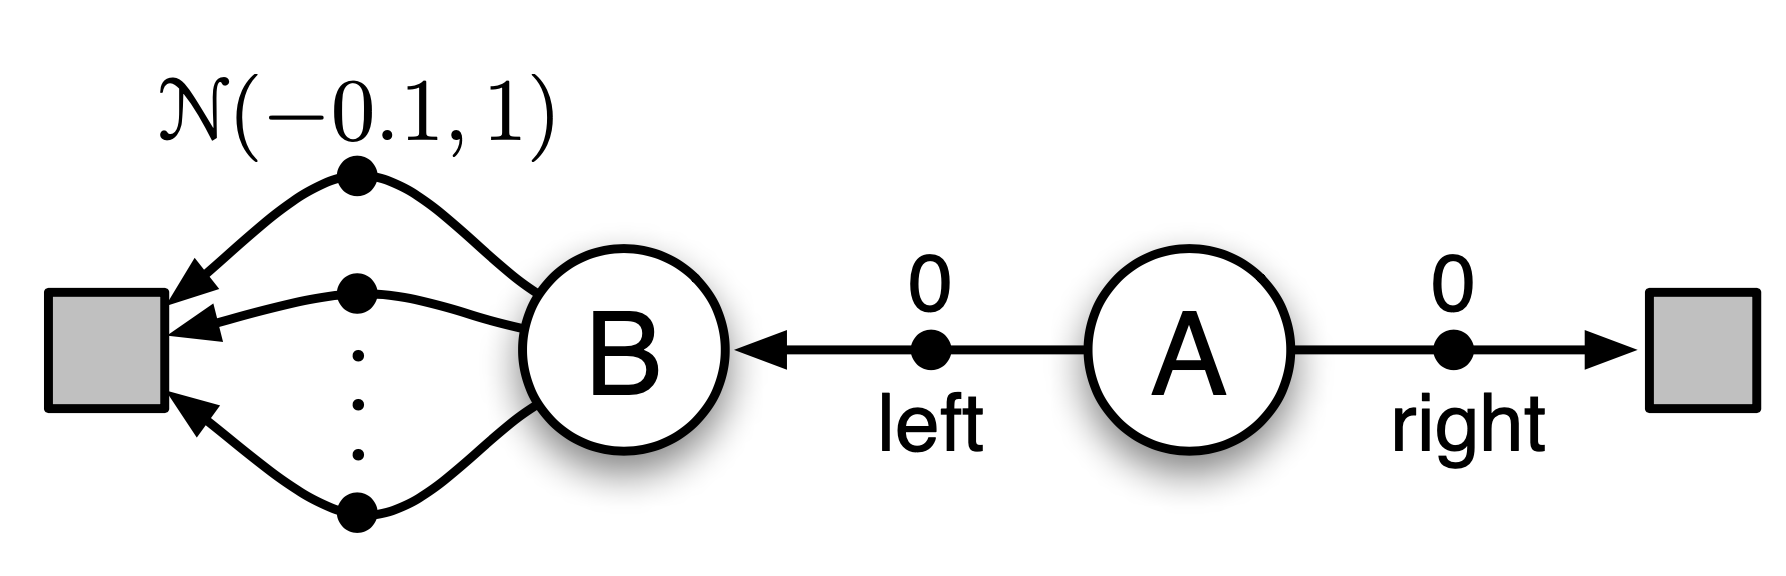
\includegraphics[width=0.3\textwidth]{figures/rl_tabular_methods_maximization_bias.png}
		\caption{Example environment where the maximization bias can lead to a suboptimal policy.}
		\label{fig:rl_tabular_methods_maximization_bias}
	\end{figure}

	\item To overcome this bias, we have to prevent to take the maximum of the estimates as an estimate of the maximum of the true values. So, intuitively, we need to determine the maximizing action from somewhere else than our estimates we are trying to update.
	\item A simple method of doing so is \textbf{Double Q-Learning}. Instead of learning a single $q$-function, we learn two, almost independently. Now, we can update $Q_1$ by using the maximum operator over $Q_2$, and vice versa. By that, we overcome the positive bias as even if $Q_1$ and $Q_2$ are biased themselves, they are positively biased on different actions. 
	\item The general update rule is then:
	\begin{equation*}
		\begin{split}
			\text{Either update }Q_1: \hspace{2mm} Q_1(S_t,A_t) & \leftarrow Q_1(S_t,A_t) + \alpha\left[R_{t+1}+\gamma Q_2\left(S_{t+1},\arg\max_a Q_1(S_{t+1},a)\right)-Q_1(S_t,A_t)\right]\\
			\text{Or update }Q_2: \hspace{2mm} Q_2(S_t,A_t) & \leftarrow Q_2(S_t,A_t) + \alpha\left[R_{t+1}+\gamma Q_1\left(S_{t+1},\arg\max_a Q_2(S_{t+1},a)\right)-Q_2(S_t,A_t)\right]
		\end{split}
	\end{equation*}
	where we randomly assign a sample either to $Q_1$ or $Q_2$ (but not both, because we otherwise get the same bias).
\end{itemize}

\subsubsection{N-step TD learning}
\begin{itemize}
	\item As we will discuss in Section~\ref{sec:value_based_tabular_difference_TD_MC} in detail, both MC and TD have certain advantages and drawbacks. However, we can actually interpolate between these two, which we call $n$-step TD (a generalization of TD(0))
	\item Instead of bootstrapping on the next state, we could use the reward of the $R_{t+2}$ as well, and then bootstrap on $v(S_{t+2})$. This leads to $2$-step TD. It gets obvious, that if we bootstrap always on the terminal state, meaning $\infty$-TD, we arrive at MC as the value of a terminal state is zero. So, we approximate the return $G_{t:t+n}$ for $n$-step TD by:
	$$G_{t:t+n} = R_{t+1}+\gamma R_{t+2} + ... + \gamma^{n-1}R_{t+n} + \gamma^n v_{t+n-1}(S_{t+n})$$
	The update rule is hence:
	$$v_{t+n}(S_t) = v_{t+n-1}(S_t) + \alpha \left[G_{t:t+n}- v_{t+n-1}(S_t)\right]$$
	\item Which $n$ works best, depends on the environment (see Section~\ref{sec:value_based_tabular_difference_TD_MC} for more detailed discussion)
	\item To enable off-policy learning, we would require importance sampling as in MC which can introduce additional variance. However, there is an alternative in $n$-step, namely the $n$-step \textbf{Tree Backup} algorithm
	\item In $n$-step tree backup, we take the next $n$ steps into account, but at each action decision, we also look at all other actions. As visualized in Figure~\ref{fig:rl_tabular_methods_n_step_tree_backup}, we now have multiple leaf nodes. At each of the leafs, we use our estimates.
	\begin{figure}[ht!]
		\centering
		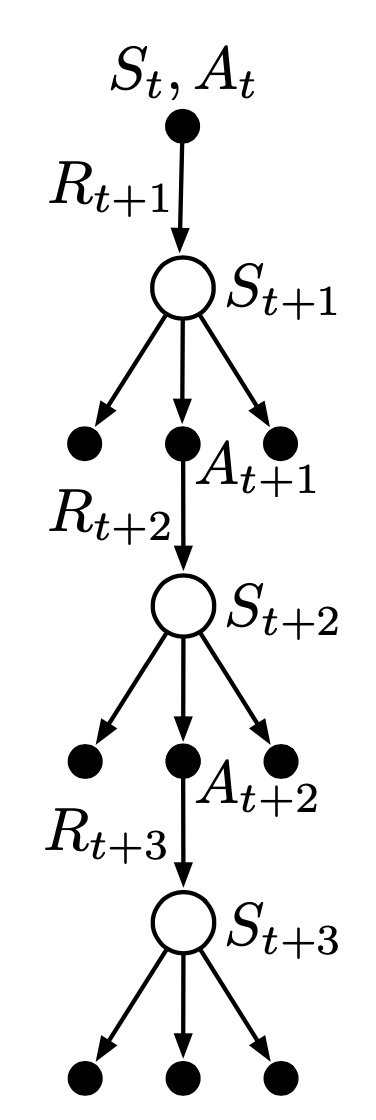
\includegraphics[width=0.1\textwidth]{figures/rl_tabular_methods_n_step_tree_backup.png}
		\caption{3-step tree backup as a backup diagram (see Section~\ref{sec:value_based_tabular_backup_diagram}).}
		\label{fig:rl_tabular_methods_n_step_tree_backup}
	\end{figure}
	\item Even if we sample from a behavior policy $p$, we can re-weight each of the leafs contribution by the target policy $\pi$. For example, at $S_{t+1}$, the leafs are weighted by $\pi(A_1|S_{t+1})$ and $\pi(A_3|S_{t+1})$, while the main sample trajectory gets a factor $\pi(A_2|S_{t+1})$. The next leafs then have $\pi(A_1|S_{t+2})\pi(A_2|S_{t+1})$ etc.
	\item For a 1-step tree backup, we get the same return estimate as for expected SARSA:
	$$G_{t:t+1}=R_{t+1}+\sum_a \pi(a|S_{t+1})Q_t(S_{t+1},a)$$
	If we have $n$ steps, we can calculate our return estimate recursively:
	$$G_{t:t+n}=R_{t+1}+ \gamma\Bigg[\underbrace{\sum_{a\neq A_{t+1}} \pi(a|S_{t+1})Q_{t+n-1}(S_{t+1},a)}_{\text{leaf contributions}} + \underbrace{\pi(A_{t+1}|S_{t+1})G_{t+1:t+n}}_{\text{samples at }t+1}\Bigg]$$
	\item Our behavior policy therefore influences where we generate longer updates, but in expectation (due to the re-weighting), we still get the correct value estimates. Hence, we can use it on off-policy data without needing importance weights ($b$ influences just the depth of certain updates)
\end{itemize}

\subsection{Comparing tabular-based methods}
\begin{itemize}
	\item We have seen now various methods and all take a slightly different approach to Reinforcement Learning
	\item In this section, we compare and review all methods, and put things into perspective
\end{itemize}
\subsubsection{Difference of TD learning and Monte Carlo}
\label{sec:value_based_tabular_difference_TD_MC}
\begin{itemize}
	\item TD can be implemented in an online, fully incremental fashion. In contrast, MC has to wait for the whole episode to finish which can delay learning in applications with very long episodes.
	\item TD learning is stronger influenced by the initial values we give the $v$/$q$-values (and hence by \underline{biased}), which can slow down training. Especially in cases where we try to learn a policy (like Q-learning for TD), we can focus our exploration in the wrong direction for a long time before finding another, optimal case.
	\item In general, MC suffer from \underline{high variance}. This is because $G_t$ is approximated by a single sample, which is often not enough for a sufficient estimate. For example, assume we have a uniform policy over two actions, and an episode is always exactly 10 steps long. Then, the expectation would give each of the $2^{10}=1024$ possibilities a weight factor of $\frac{1}{1024}$ but in MC, we simply pick one of them which clearly is inaccurate.
	\item As usual, there is a trade-off version of both, which is $n$-step TD learning. Which $n$ to choose is highly depending on your environment. For the extreme case of only having a single action to take, MC is clearly preferred because there is no variance in the updates. However, in the case where we can have many different outcomes from the same state, TD learning might be the better option. A common rule of thumb is that we need a lower learning rate for larger $n$ due to the increase of variance
	\item Another interesting difference is that (batch) MC finds the estimates that minimizes the \underline{mean-squared error} on the training set, whereas (batch) TD(0) finds the optimal estimates for a \underline{maximum-likelihood model} of the Markov process. This means that it estimates the transition probability from state $i$ to $j$ as the fraction of observed transitions from $i$ to $j$, and its expected reward is the average of the rewards observed for this transition. Thus, TD learning exploits the Markov property of the environment while MC neglects it. Note that this property can make a big difference if we observe not sufficient data points for each state.
\end{itemize}
\subsubsection{Backup diagrams}
\label{sec:value_based_tabular_backup_diagram}
\begin{itemize}
	\item Another way to visualize the difference between TD and MC is the usage of \textit{backup diagrams}
	\item A backup diagram visualizes a sequence of actions (black dots) and states (white nodes). We always go from a state to a action, which leads us to a next state. One example diagram was already given in Figure~\ref{fig:rl_tabular_methods_n_step_tree_backup}.
	\item Now, consider Figure~\ref{fig:rl_tabular_methods_final_comparison} where we visualize the different extreme cases. TD learning has a shallow update (bootstraps on the next state), while Monte Carlo has infinite depth (i.e. going until the end). The trade-off here is obviously the variance/bias so that $n$-step TD is in between those.
	
	\begin{figure}[ht!]
		\centering
		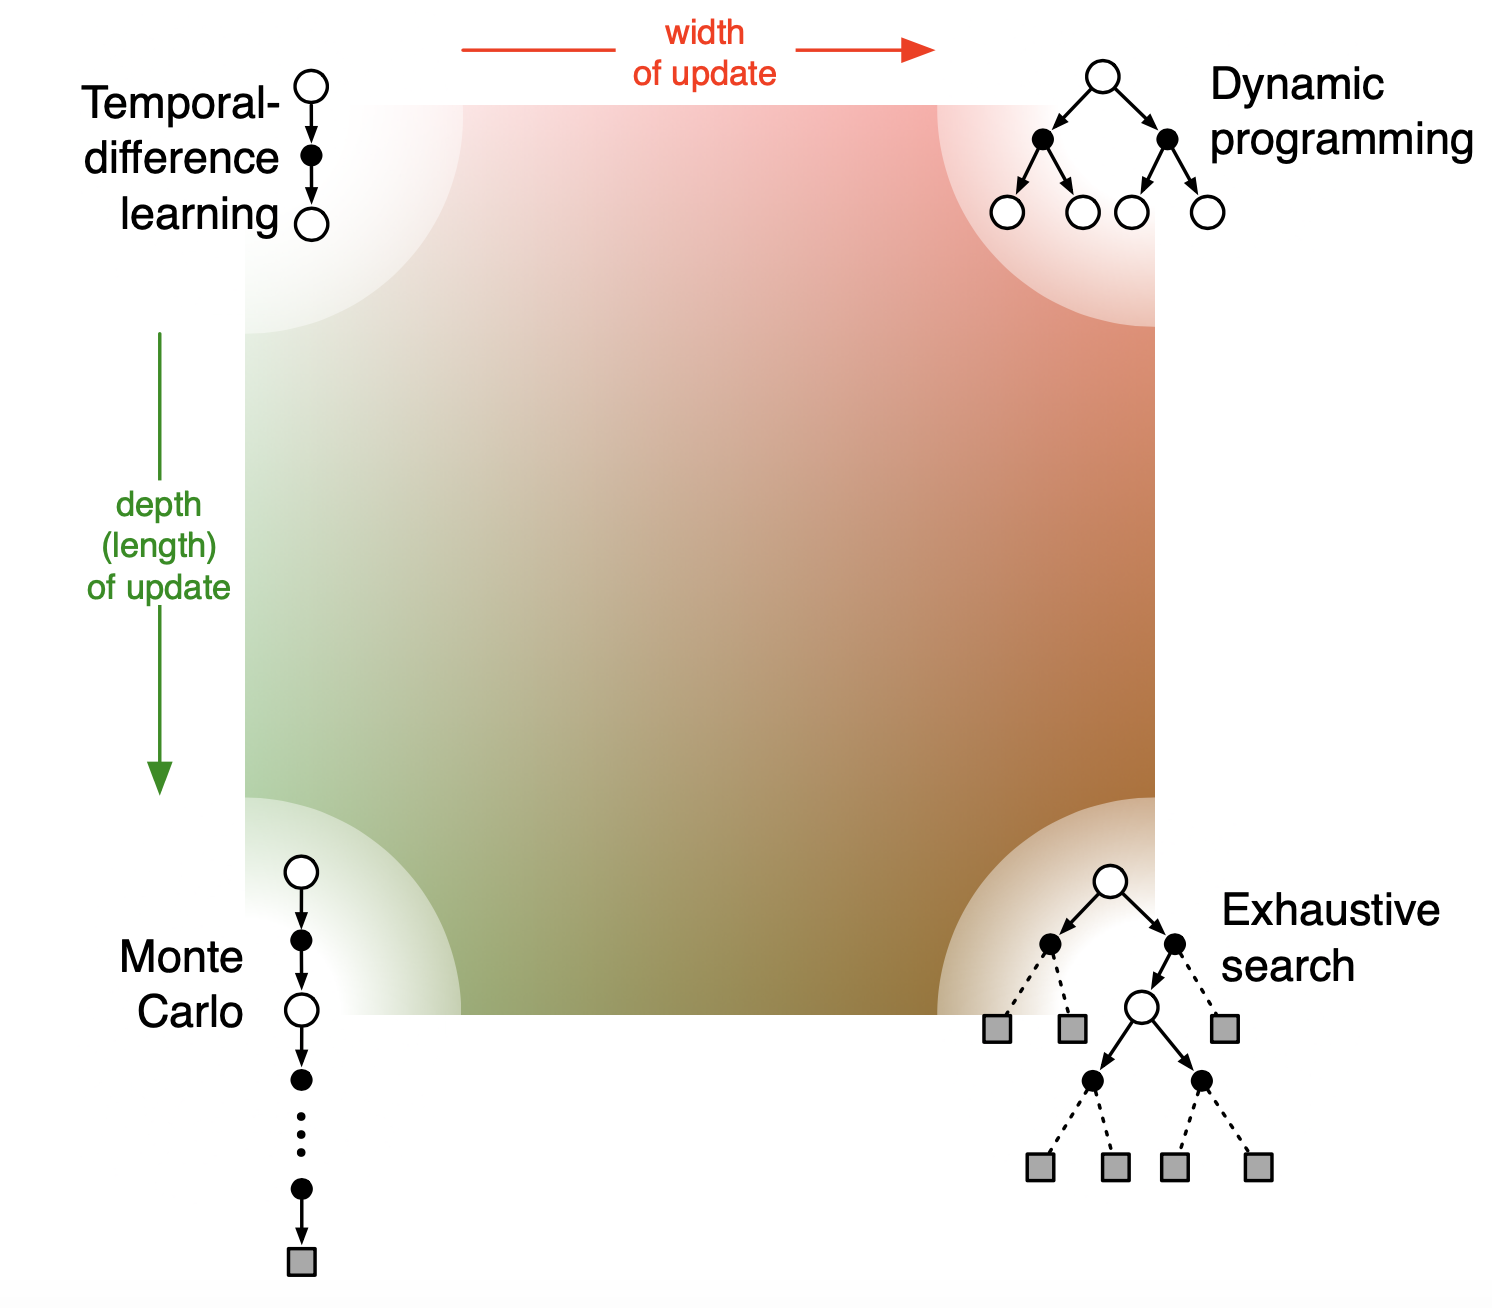
\includegraphics[width=0.4\textwidth]{figures/rl_tabular_methods_final_comparison.png}
		\caption{Putting all methods so far into perspective.}
		\label{fig:rl_tabular_methods_final_comparison}
	\end{figure}
	
	To the right, we get \textit{wider} updates, i.e. move from sampled updates towards expected updates. This means that we consider more actions and states we can end up in. Dynamic programming uses the whole environment dynamics, hence it takes all possible actions and next states into account. In between TD and DP, we can consider expected SARSA or Q-learning as they look at the next actions, but use bootstrapping. 
	
	If we make those methods deeper, we arrive at the $n$-step tree backup algorithm. Making dynamic programming deeper means that we consider \textbf{all} possible outcomes from a given state, which includes possible actions we can get, and possible next states we can end up in. This obviously ends up in a huge, intractable graph for most environments (if we even have given the dynamics) so that it is mostly not feasible to perform.
\end{itemize}
\subsubsection{Limitations so far}
\begin{itemize}
	\item To summarize the tabular-based methods, we want to review their limitations so far.
	\item First of all, as the name indicates, for all the previous methods we store the $q$- and $v$-functions as a table. This is however not always possible. Suppose we have a continuous state space. Then we cannot create a table for that. Alternatively, imagine we want to play an Atari game. Having a screen resolution of $256\times 256$, we would get $256\times 256\times 3\times 256$ different frames (last two factors are channels and 8-bit values of channels) making it infeasible to store. However, it would be also extremely inefficient because similar frames mostly relate to similar actions to take. This leads us to approximate value-based learning methods which we will review in Section~\ref{sec:value_based_approximation}.
	\item Currently, we have to choose the (behavior) policy ourselves with which we explore the environment. Furthermore, if we want to learn an optimal stochastic policy, we also need to set $\epsilon$ in $\epsilon$-soft policies, or the temperature for softmax distributions. But not only for exploration we want randomness, as in partially observable states, we also have uncertainty which we have to take into account. The question arises whether we cannot learn the optimal stochasticity in the algorithm itself, which we will discuss in Section~\ref{sec:policy_learning} and \ref{sec:partially_observable}.
	\item Until we have learned what the effect of our actions are, it takes quite some time for TD and MC to learn. If we want to take sample efficiency into account, we might want to consider model-based approaches as it will be discussed in Section~\ref{sec:model_based}.
\end{itemize}
\newpage
\section{Value-based RL: Learning with approximation}
\label{sec:value_based_approximation}
\textit{This section reviews the lecture slides 5 and 6.}
\begin{itemize}
	\item When we talk about approximating the value function, we mean that instead of implementing $v$ as look-up table, we view it as parameterized function $\hat{v}(\bm{w},s)\approx v_{\pi}(s)$ with $\bm{w}\in\R^{d}$.
	\item Commonly, we try to allow generalization over nearby states while trying to keep it compact. Hence, the size of the weights,  $d$, is mostly much smaller than the actual state size. This implies that a change in $\bm{w}$ will affect many states, and hence, generalize.
	\item Learning value functions is similar to supervised learning as we try to push a prediction closer to a target (similar to regression). The value error can be summarized as:
	$$\overline{\text{VE}}(\bm{w}) = \sum_{s\in S}\mu(s)\left[v_{\pi}(s)-\hat{v}(s,\bm{w})\right]^2=\E_{s\sim\mu(s)}\left[\left(v_{\pi}(s)-\hat{v}(s,\bm{w})\right)^2\right]$$
	where $\mu(s)$ is a weighting factor for the states (which state is how important, distribution over those). This depends on the task we are aiming for.
	
	However, keep in mind that our overall goal is to find the optimal policy, and not the best value function. So, the VE error might not be optimal as we often converge to local optima. 
\end{itemize}
\subsection{Types of function approximations}
\begin{itemize}
	\item There are various function approximation techniques we can use. We will review here a few, practical/simple ones
	\item In general, we distinguish between linear and non-linear function approximation. We call an approximation linear if the value function is linear with respect to the weight, namely:
	$$\hat{v}(s,\bm{w})=\bm{w}^T\bm{x}(s)$$
	where $\bm{x}(s)$ can be any (non-)linear functions. It can be also seen as a linear combination of static feature extractions. Some examples for $\bm{x}$ are:
	\begin{itemize}
		\item \textit{Polynomials}, as if we take enough (infinite), we would be able to approximate any function. However, this is not feasible so we mostly have many features (especially in higher dimensions because we have $\left[1,s_1,s_2,s_1^2, s_2^2, s_1s_2, s_1^2s_2,...\right]$), and hence less generalization. Furthermore, the behavior at 0 is rather static
		\item \textit{Aggregations} where we group multiple states into one. This can be seen as returning a one-hot vector for $\bm{x}$ where the $1$ assigns a point to a certain state group. Figure~\ref{fig:rl_approximate_value_based_aggregation} visualizes some examples.
		\begin{figure}[ht!]
			\centering
			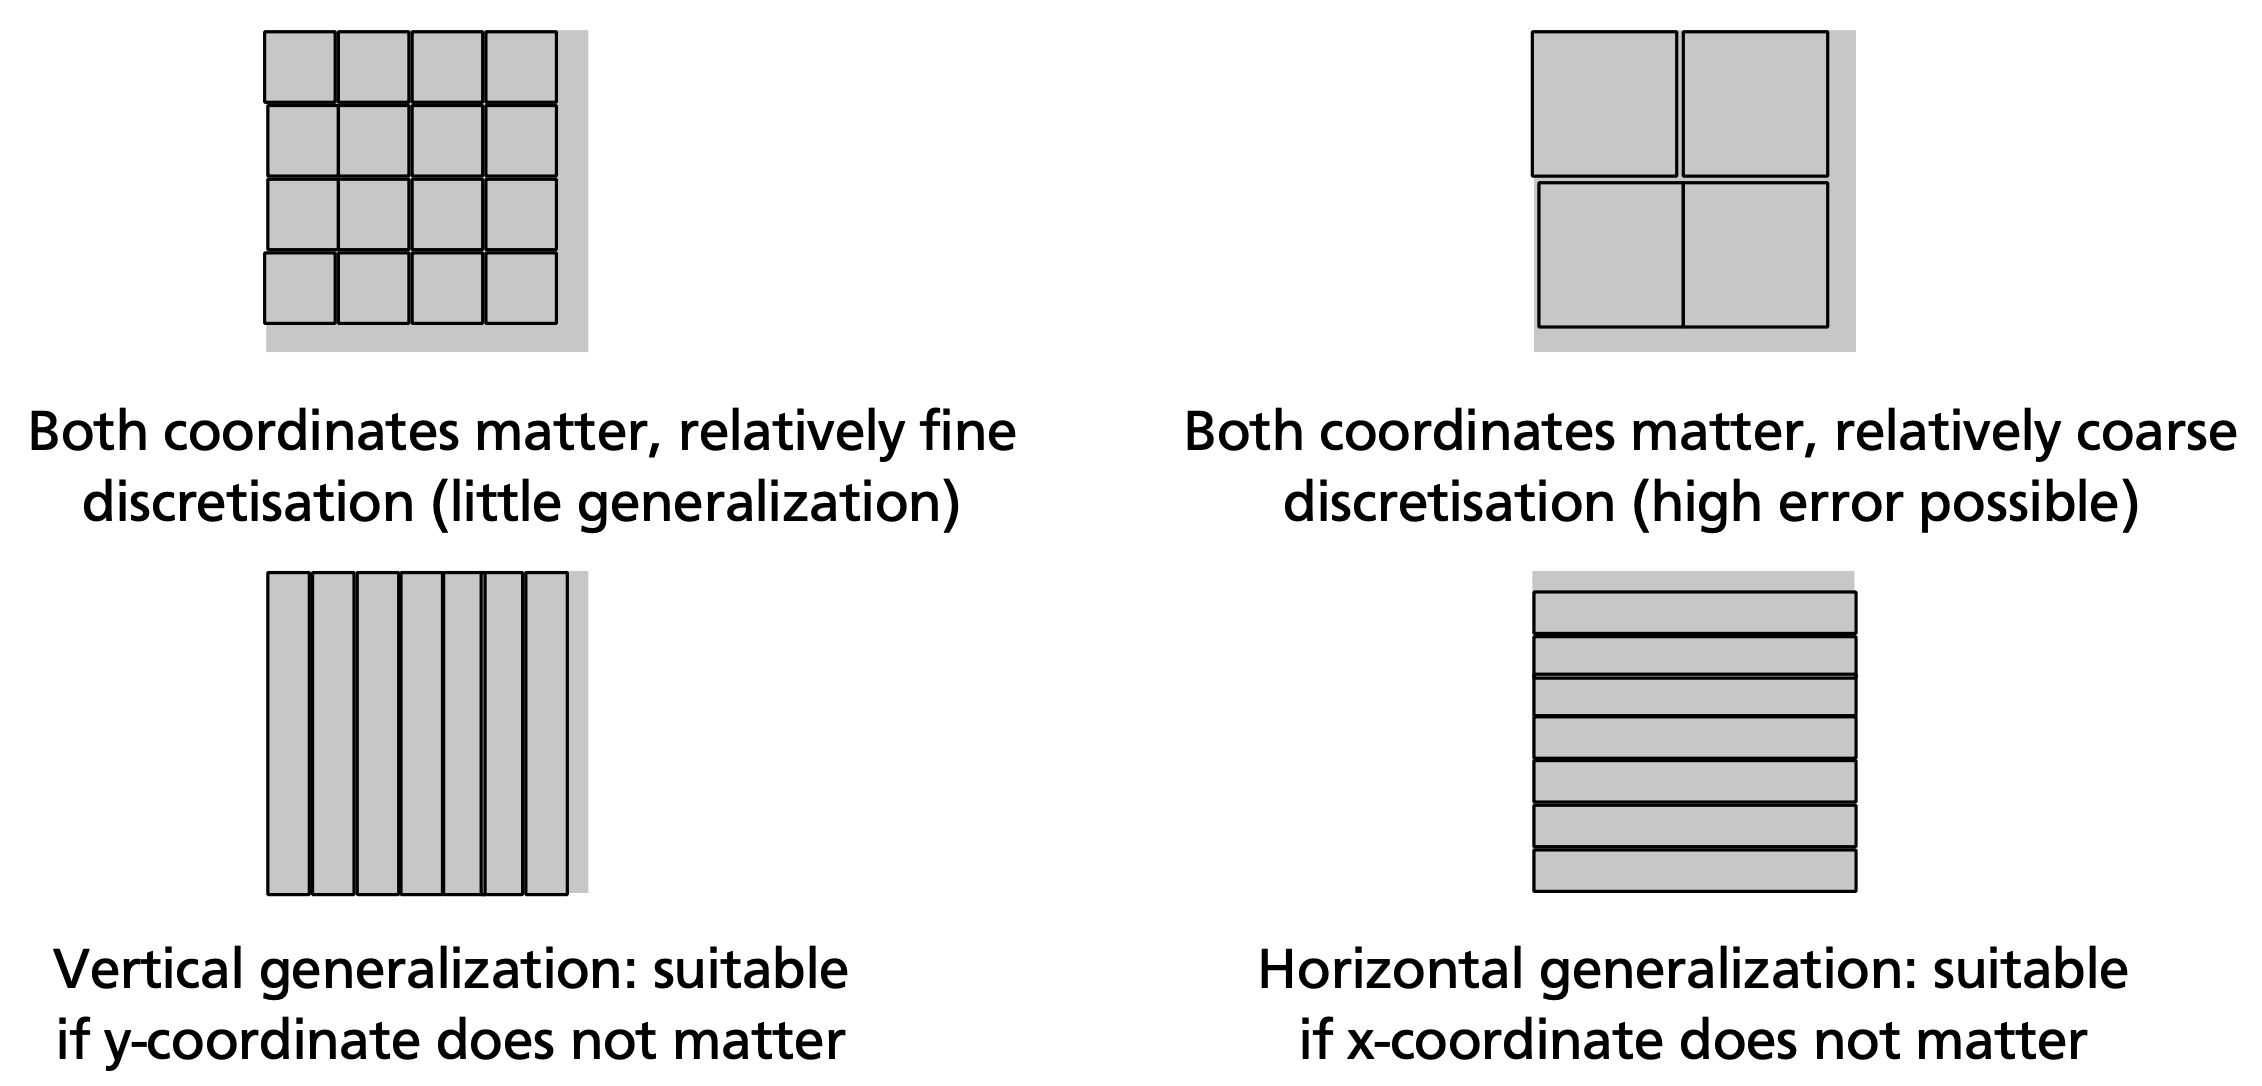
\includegraphics[width=0.5\textwidth]{figures/rl_approximate_value_based_aggregation.png}
			\caption{Simple types of aggregations on a 2D state space. Note that we can combine aggregations, meaning that we use both a vertical and a horizontal aggregation.}
			\label{fig:rl_approximate_value_based_aggregation}
		\end{figure}
		\item \textit{Radial basis functions} that takes the distance to a mean in the state space, e.g. $||\mu_i-s||$, as input features. We can model this by having multiple Gaussian, and weight their influence by $p(s)$. It enables us to have smoother transitions between close-by states, but might be problematic for far-away states. This is why it is often problematic in high-dimensional state spaces.
		\item \textit{Fourier basis} where we take different frequencies to model $s$. This can provide a quite flexible feature set.
	\end{itemize}
	Note that tabular RL can also be expressed by linear function approximation where we simply use $\bm{x}(s)=\left[\delta(s=s_1), \delta(s=s_2),...\right]$, and $\bm{w}$ therefore contains one parameter per state.
	
	Linear function approximation is especially used when prior knowledge can be introduced in the system. Carefully selecting the features simplifies the learning objective of the model, and hence, let it converge faster.
	
	\item In non-linear function approximation, we use $\bm{w}$ in a non-linear fashion in $\hat{v}$, such as in neural networks.
	
\end{itemize}
\subsection{Prediction objective for on-policy prediction}
\begin{itemize}
	\item In the case that we perform a on-policy prediction (i.e. policy evaluation for a fixed policy), the state importance is based on the visit frequency of $\pi$. To arrive at $\mu$, we also have to distinguish between the tasks:
	\begin{itemize}
		\item If we have a continuing task (never ending), we get a stationary distribution at the point:
		$$\mu_{\pi}(s)=\sum_{s'}\sum_{a}p(s|s',a)\pi(a|s')\mu_{\pi}(s')$$
		with the condition that we can reach every state from the start.
		\item For episodic tasks, we need to consider the start frequency $h(s)$ as well. To guarantee that $\mu(s)$ is a distribution, we can use a softmax:
		$$\mu_{\pi}(s)=\frac{\eta(s)}{\sum_{s'}\eta(s')}, \hspace{4mm}\eta(s)=h(s)+\sum_{s'}\sum_a p(s|s',a)\pi(a|s')\eta(s')$$
		where the second part is pretty much the same as before.
	\end{itemize} 
	\item In order to calculate the gradients $\nabla_{\bm{w}}\overline{\text{VE}}(\bm{w})$, we would need to know $\mu(s)$ which is not possible due to missing information of the environment dynamics ($p(s'|s,a)$). However, we can approximate it by Monte-Carlo samples such that:
	$$\nabla_{\bm{w}}\overline{\text{VE}}(\bm{w})\approx \nabla_{\bm{w}}\left[G_t - \hat{v}(S_t,\bm{w})\right]^2 = -2\cdot \left[G_t - \hat{v}(S_t,\bm{w})\right] \nabla_{\bm{w}}\hat{v}(S_t,\bm{w})$$
	Which leads us to the \textbf{Gradient Monte Carlo} algorithm:
	$$\bm{w}_{t+1}=\bm{w}_{t}+\alpha \left[G_t - \hat{v}(S_t,\bm{w})\right] \nabla_{\bm{w}}\hat{v}(S_t,\bm{w})$$
	\item Alternatively, we could also think about using the bootstrapping estimate as target, which gives us the following update rule:
	$$\bm{w}_{t+1}=\bm{w}_t + \alpha\underbrace{\left[R_{t+1} + \gamma\hat{v}(S_{t+1},\bm{w}_t) - \hat{v}(S_t,\bm{w}_t)\right]}_{\text{TD error }\delta}\nabla_{\bm{w}}\hat{v}(S_t,\bm{w}_t)$$  
	This method is called \textbf{Semi-gradient TD(0)}, and indicates by its name that it is not a true gradient. The reason for that is that we actually ignore the dependency of the target on $\bm{w}$. We assume it to be fixed.  Nevertheless, experiments with the true gradient have shown that the semi-gradient works much better in practice. We will discuss it later in more detail.
	
	Note that as in the value-based, we can extend this approach to $n$-step if wanted.
	\item When comparing Gradient MC and semi-gradient TD(0), we get the same arguments as for the tabular case in Section~\ref{sec:value_based_tabular_difference_TD_MC} $\Rightarrow$ TD has lower variance and learns usually faster, but can have a bias (see below)
	\item A thing to keep in mind when using semi-gradient TD(0) is that it tries to minimize distance between close-by states, especially if we take approximation like aggregating multiple state into the same. This is because a small step can lead to a huge TD error which we try to minimize. 
	\begin{figure}[ht!]
		\centering
		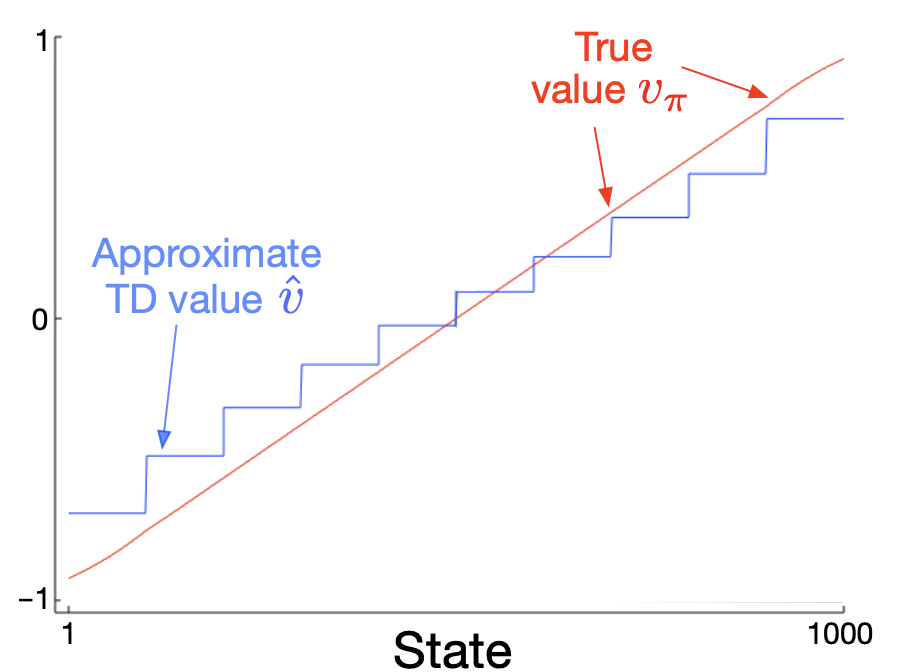
\includegraphics[width=0.4\textwidth]{figures/rl_approximate_value_based_semi_gradient_td.png}
		\caption{Problems of semi-gradient TD(0) updates on the random walk example. It prefers a value function with low changes between states, so that it gets a biased prediction.}
		\label{fig:rl_approximate_value_based_semi_gradient_td}
	\end{figure}
\end{itemize}
\subsubsection{Discussion on convergence for different objectives}
\begin{itemize}
	\item The advantages of linear function approximations are that the gradients are easy to calculate ($\nabla_{\bm{w}}\hat{v}(s,\bm{w})=\bm{x}(s)$). Furthermore, it can be proven that all local optima are global optima, so that gradient MC converges to the minimum of $\overline{\text{VE}}$. This is not necessarily the case for semi-gradient TD but we can define a upper bound $\overline{\text{VE}}(\bm{w}_{td})\leq \frac{1}{1-\gamma}\min_{\bm{w}}\overline{\text{VE}}(\bm{w})$ and guarantee that it converges. 
	
	In the non-linear case, we cannot guarantee convergence for semi-gradient TD (but for Gradient Monte Carlo), and we might end up in local optima. Nevertheless, linear features are much more restricted than non-linear as neural networks. Hence, non-linear methods can lead to better results, even if we might get stuck in local optima.
	
	\item When learning via Gradient Monte Carlo or Semi-gradient TD, we have to select a step size $\alpha$. This can be a bit more tricky here because we combine the values of many states into a single function. In case of linear function approximation, we can actually give a rule of thumb because the features are static, namely:
	$$\alpha = (\tau\E[\bm{x}^T\bm{x}])^{-1}$$
	where $\tau$ is the number of experiences we expect to have for the same (or similar) feature vector to average over (as say the learning rate you would choose for the tabular setting would be $\frac{1}{\tau}$)
	\item Alternatively we could try to find the fix point of semi-gradient TD(0). We can write the TD update rule for linear function approximation as:
	\begin{equation*}
		\begin{split}
			\bm{w}_{t+1} & = \bm{w}_t + \alpha \left(R_{t+1}+\gamma \bm{w}_t^T \bm{x}_{t+1} - \bm{w}_t^T\bm{x}_t\right)\bm{x}_t\\
			& = \bm{w}_t + \alpha \left(R_{t+1}\bm{x}_t - \bm{x}_t (\bm{x}_t - \gamma \bm{x}_{t+1})^T \bm{w}_t\right)\\
			\implies \E[\bm{w}_{t+1}|\bm{w}_t] & = \bm{w}_t + \alpha \left(\underbrace{\E[R_{t+1}\bm{x}_t]}_{\bm{b}} - \underbrace{\E[\bm{x}_t (\bm{x}_t - \gamma \bm{x}_{t+1})^T]}_{\bm{A}} \bm{w}_t\right)\\
		\end{split}
	\end{equation*}
	The fix point is given when we do not change our weights anymore, meaning $\bm{w}_{t+1}=\bm{w}_t$. This is the case if:
	$$\bm{w}_{td}=\bm{A}^{-1}\bm{b}$$
	We can approximate $\bm{A}$ and $\bm{b}$ by MC sampling:
	\begin{equation*}
		\begin{split}
			\hat{\bm{A}}_t & = \sum_{k=0}^{t-1}\bm{x}_k\left(\bm{x}_k - \gamma\bm{x}_{k+1}\right)^T + \epsilon\bm{I}\\
			\hat{\bm{b}}_t & = \sum_{k=0}^{t-1}R_{k+1}\bm{x}_k
		\end{split}
	\end{equation*}
	where $\epsilon$ is a small constant ensuring that $\bm{\hat{A}}$ is always invertible. This solution is called \textbf{least-squares temporal-difference (LSTD)}, and is usually more sample efficient because we do not have to perform iterative updates, and has the benefit of not requiring a step size. However, it is more computationally expensive (quadratic plus the invert of $\bm{A}$), and we cannot adapt to a change in the environment over time (once performed, we fix our weights)
\end{itemize}
\subsection{Control with approximation}
\begin{itemize}
	\item For learning a policy $\pi$, we again change our objective to learning the $q$-values, which we now approximate with $\hat{q}(s,a,\bm{w})$. We will focus on episodic cases, but note that everything could be generalized to the continuous case as well.
	\item In the \textbf{on-policy} case, we can use methods like (episodic) semi-gradient SARSA, so that our update step is:
	$$\bm{w}_{t+1}=\bm{w}+\alpha\left[U_t - \hat{q}(S_t,A_t,\bm{w})\right]\nabla_{\bm{w}}\hat{q}(S_t,A_t,\bm{w})$$
	where $U_t$ is our target, which is for one-step SARSA $U_t = R_t + \gamma \hat{q}(S_{t+1},A_{t+1},\bm{w})$.
	As usual, we iterate over this update rule while setting our policy to $\epsilon$-greedy on $\hat{q}$.
	\item In the \textbf{off-policy} case, we experience more problems. As we have a behavior policy $b$ and target policy $\pi$, we need to use importance weight to correct the target of the update:
	$$\bm{w}_{t+1}=\bm{w}+\rho \alpha\left[U_t - \hat{q}(S_t,A_t,\bm{w})\right]\nabla_{\bm{w}}\hat{q}(S_t,A_t,\bm{w})$$
	Although it increases variance, it is necessary to guarantee unbiased, correct estimates.
	
	The second issue is that we need to take the changed state distribution, $\mu_b$, into account. Consider for example the very simple MDP in Figure~\ref{fig:rl_approximation_value_based_offpolicy_divergence} for which we just want to estimate $v$ (policy evaluation). We assume the reward for any action to be $0$, and start with an initial value of $w=10$.
		
	\begin{figure}[ht!]
		\centering
		
\includegraphics[width=0.2\textwidth]{figures/rl_approximation_value_based_offpolicy_divergence.png}
		\caption{Simple MDP where off-policy updates can diverge. Green indicate behavior policy, red the target. Every transition has a reward of $0$, meaning that the optimal $v$ are 0 at both states.}
		\label{fig:rl_approximation_value_based_offpolicy_divergence}
	\end{figure}
	
	First, consider the on-policy case where $\pi=b$ (green action from second state). Then, we would alternate between the two update equations:
	\begin{equation*}
		\begin{split}
		\text{Left to right: }\hspace{2mm}w_{t+1} & = w_t + \alpha (\gamma \cdot 2w_t-w_t)\nabla_w w_t = (1+\alpha(2\gamma-1)) w_t\\
		\text{Right to left: }\hspace{2mm}w_{t+1} & = w_t + \alpha (\gamma w_t-2w_t)\nabla_w 2w_t = (1+2\alpha(1-2\gamma)) w_t\\
		\end{split}
	\end{equation*}
	Overall, we would converge to $w=0$ as the right to left update is twice as high as the other.
	
	Now, assume the behavior policy stays the same, but our target policy stays at the second state. Then, the importance weight for left to right is 1 (as both policies do that with probability 1), but from right to left is zero because we would not take this action with our target policy. So we end up with the update:
	\begin{equation*}
		\begin{split}
			\text{Left to right: }\hspace{2mm}w_{t+1} & = w_t + \alpha (\gamma \cdot 2w_t-w_t)\nabla_w w_t = (1+\alpha(2\gamma-1)) w_t\\
		\end{split}
	\end{equation*}
	which makes $w_t$ head to infinity if $\gamma>0.5$. This shows that off-policy prediction can diverge!
	
	\item This divergence can occur when the following three methods are used together (\textit{Deadly Triad}):
	\begin{itemize}
		\item Function approximation
		\item Semi-gradient bootstrapping
		\item Off-policy training
	\end{itemize}
	\item To overcome this issue, we need to consider alternatives to semi-gradients.
	
\end{itemize}
\subsubsection{Alternatives to semi-gradients}
\begin{itemize}
	\item There are couple of objectives that we can use instead of semi-gradient. We visualize all of them in Figure~\ref{fig:rl_approximation_value_based_different_errors}, and discuss them here in detail
	\begin{figure}[ht!]
		\centering
		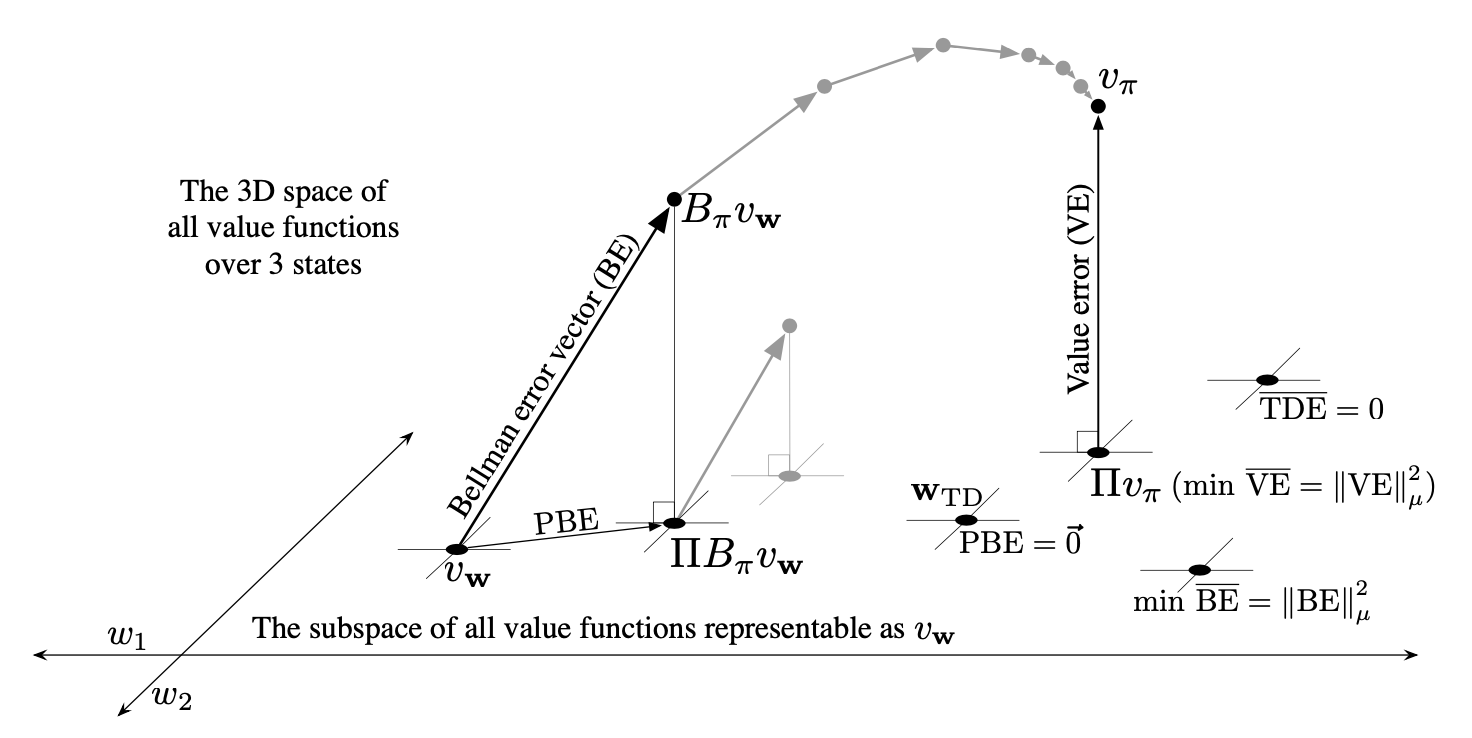
\includegraphics[width=0.6\textwidth]{figures/rl_approximation_value_based_different_errors.png}
		\caption{Geometry of linear value-function approximation. We show an approximation of a 3D state space by a two dimension weight vector.}
		\label{fig:rl_approximation_value_based_different_errors}
	\end{figure}
	
	\item Before we start our discussion, we need to introduce some notation:
	\begin{itemize}
		\item First, we need to consider how we measure distance between two value functions. The standard euclidean norm is not sufficient, as we give importance to different states. This is why we take $\mu$ into account:
		$$||v_1-v_2||_{\mu}^2 = \sum_{s\in\mathcal{S}} \mu(s)\left[v_1(s)-v_2(s)\right]^2$$
		\item Given the norm, we also want to define a \textit{projection operator} which assign to an arbitrary $v$ (over whole state space) the closest value function based on the norm that can be represented:
		$$\Pi v = v_{\bm{w}}\hspace{3mm}\text{where}\hspace{3mm}\bm{w}=\arg\min_{\tilde{\bm{w}}}||v-v_{\tilde{\bm{w}}}||_{\mu}^2 $$
		\item The last notation we want to introduce is the Bellman operator, which maps a value function $v$ to its bootstrapping estimates:
		$$(B_{\pi}v_{\bm{w}})(s) = \sum_a \pi(a|s)\sum_{s',r}p(s',r|s,a)[r+\gamma v_{\bm{w}}(s')] = v_{\bm{w}}(s) + \overline{\delta}_{\bm{w}}(s)$$
		with $\overline{\delta}_{\bm{w}}(s)$ being the expected TD error for state $s$.
	\end{itemize}
	\item The value error $\overline{\text{VE}}$ is minimized if the norm is the lowest to $v_{\pi}$: $$\min_{\bm{w}} \overline{\text{VE}}(\bm{w}) = \min_{\bm{w}} ||v_{\bm{w}}-v_{\pi}||_{\mu}^2 $$
	The projected point, which we can actually reach, is $\Pi v_{\pi}$ which is the best point we can represent in our $\bm{w}$-space. Gradient Monte Carlo methods converge to this point, but mostly quite slowly
	\item Without the approximation, we could simply apply the Bellman operator  over and over again, and reach $v_{\pi}$ (as in tabular TD(0) learning) which is the gray line above. However, we cannot represent the change so that we have to project $v$ after each step: $\Pi B_{\pi}v_{\bm{w}}$. The step we take in between is the projected Bellman error $PBE=\Pi\delta_{\bm{w}}$ 
	
	Semi-gradient TD is converging to the point where $PBE=0$ as we reach a fix-point there. However, this does not have to be where the minimum Bellman error is reached because imagine $\delta_{\bm{w}}$ being orthogonal to $\bm{w}$-subspace. Then, the projected bellman error is 0, but without projection, we would continue changing $\bm{w}$, until we reach $\min \overline{\text{BE}}$.
	
	At the same time, even if we would reach $\min \overline{\text{BE}}$, it would be most likely not be a optimum (i.e. gradients greater than zero) because the gradients can point to outside the representable $\bm{w}$-space (does not need to be orthogonal as before), and hence the projected Bellman error can be unequals zero.
	
	\item The last objective we consider here is the true-gradient TD error, meaning: $$\overline{\text{TDE}}(\bm{w})=\sum_{s\in\mathcal{S}}\mu(s)\E\left[\delta_t^2 |S_t=s,A_t\sim \pi\right] = \E_{b}[\rho_t \delta_t^2] \hspace{4mm}\text{(if we assume $\mu$ is under $b$)}$$
	Following SGD updates, we get:
	$$\bm{w}_{t+1}=\bm{w}_t + \alpha \rho_t \delta_t (\nabla \hat{v}(S_t,\bm{w}_t) - \gamma \nabla \hat{v}(S_{t+1},\bm{w}_t))$$
	
	\item Now, let's consider which of these objectives we can take as alternative to semi-gradient updates. 
	
	A major drawback of TDE is that we also take the gradients regarding the next steps, which can push the value function in a wrong direction (tries to minimize distance between the steps, similar to Figure~\ref{fig:rl_approximate_value_based_semi_gradient_td}). Consider the MDP in Figure~\ref{fig:rl_approximation_value_based_TDE}, with on-policy evaluation of a uniform policy, and $\gamma=1$.
	
	\begin{figure}[ht!]
		\centering
		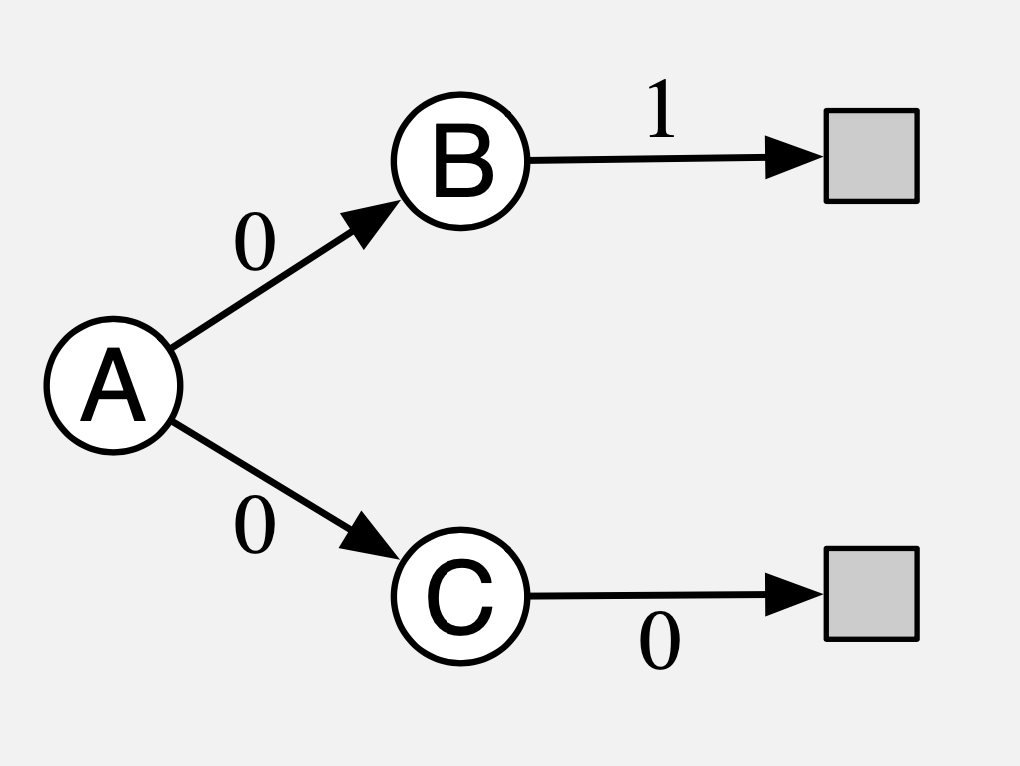
\includegraphics[width=0.2\textwidth]{figures/rl_approximation_value_based_TDE.png}
		\caption{Simple example where TDE gives an undesirable result.}
		\label{fig:rl_approximation_value_based_TDE}
	\end{figure}

	The optimal/correct value function is obviously $v(A)=1/2, v(B)=1, v(C)=0$. The TD error is given by:
	$$\delta_t=\frac{1}{2}\left(\left[v(B)-v(A)\right]^2 + \left[1-v(B)\right]^2\right)+\frac{1}{2}\left(\left[v(C)-v(A)\right]^2 + \left[0-v(C)\right]^2\right)$$
	for which the optimal is actually $v(A)=1/2, v(B)=3/4, v(C)=1/4$ because we also minimize the distance between $v(A)$ and $v(B)$, and similarly between $v(A)$ and $v(C)$.
	
	\item For calculating the Bellman error ($\min \text{BE}$), we need to calculate:
	$$\overline{\text{BE}}=||\overline{\delta}_{\bm{w}}||_{\mu}^2\hspace{2mm}\text{where}\hspace{2mm}\overline{\delta}_{\bm{w}}=\E_{\pi}\left[\delta_{\bm{w}}|S_t=s,A_t\sim\pi\right]$$
	As we have the square in the error, to guarantee an unbiased estimate, we need to sample at least two times independently (otherwise we estimate $\E[\delta^2]$ instead of $\E[\delta]^2$). This is mostly not possible in interactions to obtain, or makes the algorithm rather slow.
	
	\item The last remaining objective is the mean squared projected Bellman error $\overline{\text{PBE}}$. We can derive at the following gradient for PBE:
	$$\nabla_{\bm{w}} \overline{\text{PBE}}(\bm{w}) = 2\E[\rho_t (\gamma \bm{x}_{t+1}-\bm{x}_t)\bm{x}_t^T]\E[\bm{x}_t\bm{x}_t^T]^{-1}\E[\rho_t\delta_t\bm{x}_t]$$
	Using the same samples for all the expectations gives the same bias as the one for the Bellman error. What we can do, however, is learning some factors from all the data, namely the last two, and denote it as $\bm{v}_t=\E[\bm{x}_t\bm{x}_t^T]^{-1}\E[\rho_t\delta_t\bm{x}_t]$. Then, we can perform SGD as:
	\begin{equation*}
		\begin{split}
			\bm{v}_{t+1} & = \bm{v}_t + \beta \rho_t (\delta_t - \bm{v}_t^T \bm{x}_t)\bm{x}_t\\
			\bm{w}_{t+1} & = \bm{w}_t + \alpha \left[\rho_t (\gamma \bm{x}_{t+1}-\bm{x}_t)\bm{x}_t^T\right]\bm{v}_t
		\end{split}
	\end{equation*}
	This algorithm is called GTD2 (gradient TD) which converges to the minimum PBE for linear features. The drawbacks are that we need an additional learning rate $\beta$ (mostly greater than $\alpha$), and need to store two parameter updates.
	
	Nevertheless, as we have a guarantee of convergence for all settings, it makes GTD2 the preferred technique compared to Semi-gradient TD, except when we just want a simple method.
	\item Overall, we have the following convergence properties:
	\begin{figure}[ht!]
		\centering
		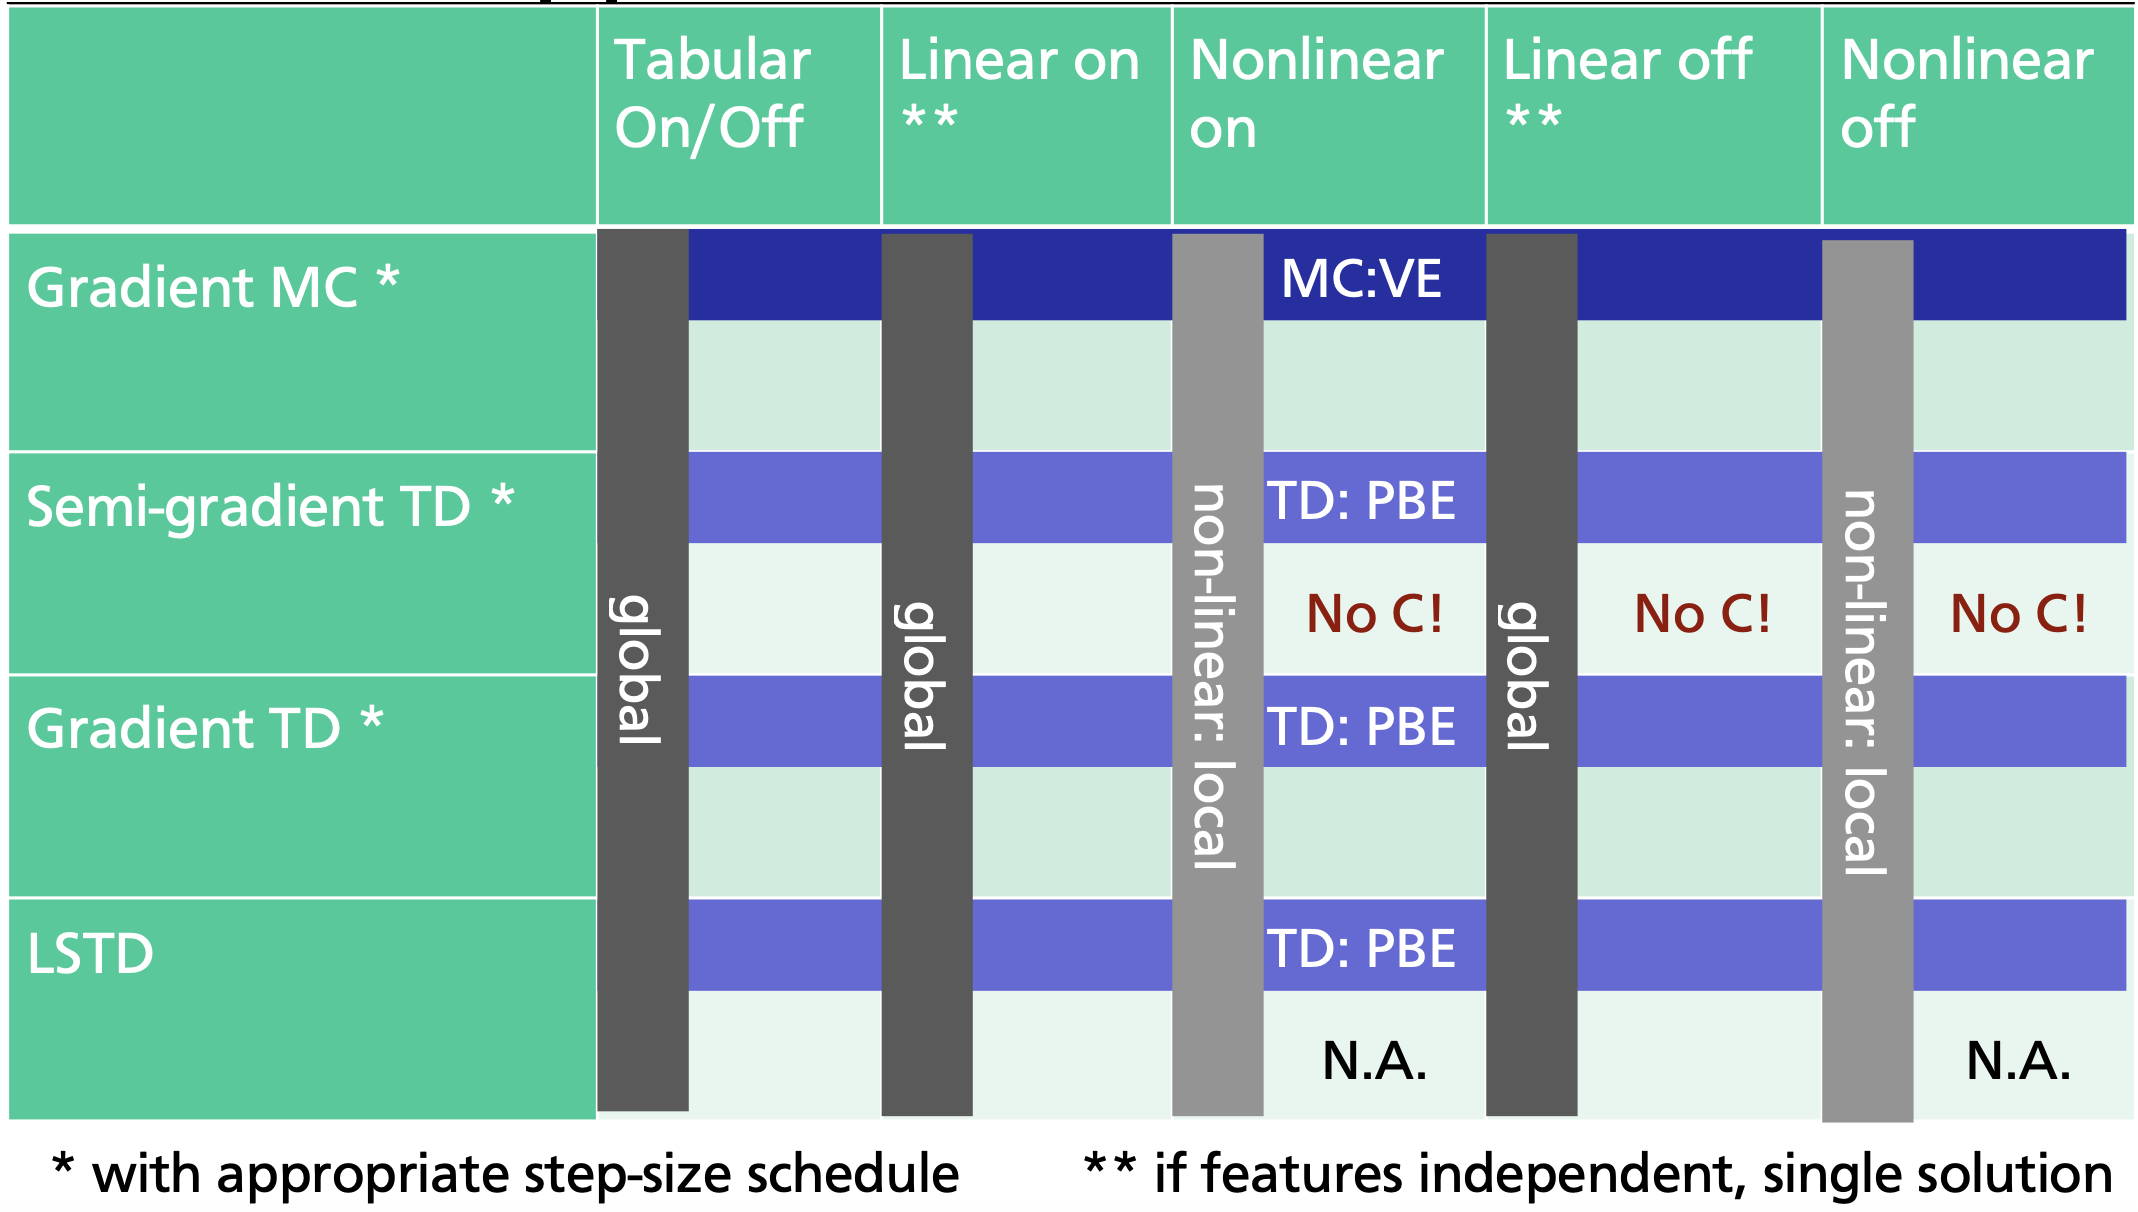
\includegraphics[width=0.6\textwidth]{figures/rl_approximate_value_based_convergence_overview.png}
		\caption{Overview of convergence properties of different optimization methods. The columns show the setting (on=on-policy, off=off-policy). "No C." for semi-gradient TD means that we cannot guarantee its convergence. "N.A" stands for "not applicable", as LSTD is based on the assumption of linear features.}
	\end{figure}	
\end{itemize}
\subsubsection{Deep Q network}
\begin{itemize}
	\item Another way of stabilizing off-policy control is by using many additional tricks, to make it more similar to supervised learning. One popular example of this is the DQN
	\item Given a state as input, we try to learn a $q$-value for each output, so that we can perform a simple maximization step over the outputs to get the optimal policy
	\item We use image as input. However, to detect movement, a couple of frames are stacked on top of each other
	\item To guarantee i.i.d. samples within a batch, and use data more efficiently (look at an experience more than once), we use \textbf{experience replay}:
	\begin{itemize}
		\item All the experiences we had from interacting with the environment are stored in a buffer (if limited size, use FIFO queue)
		\item At every time step, randomly select $N$ experiences which form a batch for training
	\end{itemize}
	Note that this is only possible because of off-policy training, as the collected experiences come from a different policy, namely an older one.
	\item Another trick to stabilize learning is \textbf{fixing the target}. As we use semi-gradient version of $q$-learning, which is:
	$$\bm{w}_{t+1}\leftarrow \bm{w}_t + \alpha \left[R_{t+1}+\gamma\max_a \hat{q}(S_{t+1}, a, \bm{w}_t) - \hat{q}(S_t, A_t, \bm{w}_t)\right]\nabla \hat{q}(S_t, A_t, \bm{w}_t)$$
	To fix the target, we copy the weights $\tilde{\bm{w}}$, and use this to calculate the target $\gamma\max_a \hat{q}(S_{t+1}, a, \bm{w}_t)$.
	
	Furthermore, it has been shown to work well to clip the TD error between a range of $[-1,1]$ to prevent any divergence issues. 
	\item If needed/wanted, we can overcome the maximization by using a double Q-learning approach
\end{itemize}






\newpage
\section{Policy gradient methods}
\label{sec:policy_learning}
\textit{This section reviews the lecture slides 7, 8, 9 and 10.}
\begin{itemize}
	\item In this section we will discuss techniques for learning the policy directly. There are couple of advantages to it:
	\begin{itemize}
		\item We are able to deal with continuous actions
		\item We are changing the policy \textit{smoothly}, meaning that after an update, we only slightly change the probability distribution over actions. In case of $\epsilon$-greedy on $q$-values, the policy heavily changes when best action becomes another one
		\item Small errors in the value functions don't give a big error in $\pi$ (we are directly optimizing the quantity of interest)
		\item We are able to include prior knowledge, like "don't fall of the cliff", "going left is potentially more interesting", etc.
		\item We are able to learn how much stochasticity is optimal for the given environment. 
	\end{itemize}
	\item In case we have discrete actions, we can simply learn by a softmax over these (viewing them as different classes). For continuous, we can for example use a Gaussian, and learn to predict its mean and variance
	\item The objective of a policy is always the same, namely optimize the expected return for its start state(s): $$J(\theta)=v_{\pi_{\theta}}(s_0)=\E\left[\sum_{t=0}^{T-1} r_{t+1}\right]$$
	Note that we assume here $\gamma=1$. We will use it throughout this section as it makes the derivations/discussion a bit easier, but we can change this term if necessary.
	\item The simplest update is using \textbf{finite difference}, meaning that we estimate the gradients by a small parameter change:
	$$\nabla J(\theta)\approx \frac{ J(\theta+\epsilon) - J(\theta-\epsilon)}{2\epsilon}$$
	However, this means that for $n$ parameters, we would need at least $2n$ roll-outs for an estimate. For stochastic policies, this estimate is extremely noisy and hence, not really applicable.
\end{itemize}
\subsection{REINFORCE and the Policy Gradient Theorem}
\begin{itemize}
	\item The Policy Gradient Theorem says that the gradients of $\nabla_{\theta}J(\theta)$ are proportional to:
	$$\nabla_{\theta}J(\theta) \propto \sum_s \mu(s) \sum_a \nabla_{\theta} \pi_{\theta}(a|s)q_{\pi_{\theta}}(s,a) $$
	Note that we are not interested in the constant proportionality factor because we will absorb it anyways in the learning rate
	\item For deriving the REINFORCE algorithm, we follow the approach of the lecture slides. Let's define $\tau$ as a trajectory that starts from $s_0$ and ends in a arbitrary terminal state. Then, the expected return is the expected return over these trajectories. Using this equality, we can derive the gradients as:
	\begin{equation*}
		\begin{split}
			\nabla_{\theta}J(\theta) & =  \nabla_{\theta} \E_{\tau}[G(\tau)]\\
			& = \int \nabla_{\theta} p_{\theta}(\tau) G(\tau)d\tau\\
		\end{split}
	\end{equation*}
	where the probability of a trajectory is defined as $p_{\theta}(\tau)=p(s_0)\prod_{t=1}^{T}\pi_{\theta}(A_t|S_t)p(S_{t+1}|A_{t},S_t)$, and $G(\tau)$ is the expected return from the initial state. Using the trick $\nabla_{\theta} p_{\theta}(\tau)=p_{\theta}(\tau)\cdot \nabla_{\theta} \ln p_{\theta}(\tau)$, we get:
	
	\begin{equation*}
		\begin{split}
			\nabla_{\theta}J(\theta) & = \int \nabla_{\theta} p_{\theta}(\tau) G(\tau)d\tau\\
			& = \E_{\tau}[G(\tau)\nabla_{\theta} \ln p_{\theta}(\tau)]\\
			& = \E_{\tau}\left[G(\tau)\sum_{t=1}^{T}\nabla_{\theta} \ln p_{\theta}(a_t|s_t)\right]\\
		\end{split}
	\end{equation*}
	\item Hence, to estimate the gradient, we can sample trajectories and approximate the expectation above. This estimate is unbiased but has some disadvantages. The efficiency of REINFORCE is low because of its high variance which comes from two points:
	\begin{itemize}
		\item First, REINFORCE can be seen as a Monte Carlo method of policy-based RL. Hence, the MC samples bring a certain level of noise with them
		\item Suppose we are playing CartPole. Our reward is 1 for each time step, until we terminate. This leads to always positive gradients, which can be seen as "supporting" the last actions. Only if we sample the other action, we might experience an even higher return which pushes the policy towards the newly explored actions. 
	\end{itemize}
	\item The second issue can be tackled by the usage of a \textit{baseline} which is a constant subtracted from the return, that does not influence the gradients being unbiased:
	\begin{equation*}
		\begin{split}
			\E_{\tau}\left[\left(G(\tau)-b\right)\sum_{t=0}^{T}\nabla_{\theta} \ln p_{\theta}(a_t|s_t)\right] & = \E_{\tau}\left[G\left(\tau\right)\sum_{t=0}^{T}\nabla_{\theta} \ln p_{\theta}(a_t|s_t)\right]  - \E_{\tau}\left[b\sum_{t=0}^{T}\nabla_{\theta} \ln p_{\theta}(a_t|s_t)\right] \\
			& = \nabla J(\theta) - b\underbrace{\int p_{\theta}(\tau)\nabla_{\theta} \ln p(\tau)d\tau}_{=0}\\
			& = \nabla J(\theta) 
		\end{split}
	\end{equation*}
	\item A good baseline is the expected reward, which we for example can aggregate over the past.
	\item However, there is one drawback which still remains. We assign each action of a trajectory the same credit, meaning that we punish every action equally no matter how much it actually was responsible for it. This is especially a problem when we punish actions for something in the past (e.g. if last 5 steps get reward of 10 each, but first got -100, we punish all of them equally). To prevent this, we move to G(PO)MDP
\end{itemize}
\subsubsection{G(PO)MDP}
\begin{itemize}
	\item Gradient estimates for (Partially Observable) Markov Decision Processes
	\item Let's reconsider the gradient estimate again, and try to split it into a part before $t$, and a part after $t$:
	
	\begin{equation*}
		\begin{split}
			\nabla_{\theta}J(\theta) & =  \E_{\tau}\left[G(\tau)\sum_{t=1}^{T}\nabla_{\theta} \ln p_{\theta}(a_t|s_t)\right]\\
			& = \E_{\tau}\left[\sum_{t=1}^{T} r_t \sum_{t'=1}^{T}\nabla_{\theta} \ln p_{\theta}(a_{t'}|s_{t'})\right]\hspace{5mm}\text{(Put in definition of return)}\\
			& = \sum_{t=1}^{T} \E_{\tau_{1:t}}\E_{\tau_{t+1:T}}\left[r_t \sum_{t'=1}^{T}\nabla_{\theta} \ln p_{\theta}(a_{t'}|s_{t'})\right]\hspace{5mm}\text{(Move sum out and split expectation)}\\
			& = \sum_{t=1}^{T} \E_{\tau_{1:t}}\left[r_t \left(\sum_{t'=1}^{t}\nabla_{\theta} \ln p_{\theta}(a_{t'}|s_{t'}) + \underbrace{\E_{\tau_{t+1:T}}\left[\sum_{t'=t+1}^{T}\nabla_{\theta} \ln p_{\theta}(a_{t'}|s_{t'})\right]}_{=\E[\int p(x)\nabla\log p(x)dx]=0}\right)\right]\\
			& = \sum_{t=1}^{T} \E_{\tau_{1:t}}\left[r_t \sum_{t'=1}^{t}\nabla_{\theta} \ln p_{\theta}(a_{t'}|s_{t'}) \right]\\
			& = \E_{\tau}\left[\sum_{t=1}^{T}  r_t \sum_{t'=1}^{t}\nabla_{\theta} \ln p_{\theta}(a_{t'}|s_{t'}) \right]
		\end{split}
	\end{equation*}
	With this rewritten gradient, we give credit for $r_t$ only those actions that came \textit{before} $t$
	\item This reduces the variance from REINFORCE, and can be combined with baselines etc. However, keep in mind that we still have a Monte Carlo sample, so that there remains a significant variance
\end{itemize}
\subsubsection{PGPE}
\begin{itemize}
	\item Even when sampling from stochastic policies during a rollout, the variation and exploration we get is mostly fairly limited. Furthermore, we end up with small perturbations (choose "left"-"right"-"left" in CartPole) which are less likely to be repeated by a deterministic policy, and can damage e.g. a robot in real-life situations
	\item Instead, we rather \textit{sample} a deterministic policy $\pi_{\theta}$ from a distribution $p(\theta|\nu)$.  The advantage is that if we now see a state twice, we can guarantee that our policy takes a same action although we are still exploring/stochastic. 
	\item So, instead of choosing $a$ at every randomly, we randomly choose the action for any state in the beginning (represented by $\pi_{\theta}$), and keep it fixed over the trajectory
	\item Our gradient (which is now with respect to $\nu$ as we want to learn $p(\theta|\nu)$) is:
	$$\nabla_{\nu} J(\nu) = \E_{\theta}\E_{\tau|\pi_{\theta}}[G(\tau) \nabla_{\nu}p(\theta;\nu)]$$
\end{itemize}
\subsection{Actor-critic Policy Gradient}
\begin{itemize}
	\item Although we increased the stability of REINFORCE by the discussed improvements, the problems of Monte Carlo sampling remain: we have to wait until the end of the episode, and the samples have a high variance
	\item First we take a look again at G(PO)MDP, where we slightly re-arrange the terms:
	$$\E_{\tau}\left[\sum_{t=1}^{T}  r_t \sum_{t'=1}^{t}\nabla_{\theta} \ln p_{\theta}(a_{t'}|s_{t'}) \right] = \E_{\tau}\left[\sum_{t'=1}^{T}\nabla_{\theta} \ln p_{\theta}(a_{t'}|s_{t'}) \sum_{t=t'}^{T}  r_t\right]$$
	In our value-based methods, we previously learn the terms $\sum_{t=t'}^{T}  r_t$ by the $v$/$q$-functions, as it is the expected value of those. Hence, we can also plug them in here:
	$$\E_{\tau}\left[\sum_{t'=1}^{T}\nabla_{\theta} \ln p_{\theta}(a_{t'}|s_{t'}) \sum_{t=t'}^{T}  r_t\right] = \E_{\tau}\left[\sum_{t'=1}^{T}\nabla_{\theta} \ln p_{\theta}(a_{t'}|s_{t'}) q_{\pi}(s_{t'},a_{t'})\right]$$
	\item The question arises whether we can replace $q_{\pi}(s_{t'},a_{t'})$ by an estimate $\hat{q}_{\bm{w}}(s_{t'},a_{t'})$ without introducing a bias. The answer is yes, but with two constraints on the function $\hat{q}_{\bm{w}}$:
	\begin{enumerate}
		\item The function has to be \textit{compatible}, which means:
		$$\nabla_{\bm{w}}\hat{q}_{\bm{w}}(s,a) = \nabla_{\theta}\ln \pi_{\theta}(a|s)\hspace{5mm}\text{like}\hspace{2mm} \hat{q}_{\bm{w}}(s,a)=\bm{w}^T \nabla_{\theta} \ln \pi_{\theta}(a|s)$$
		\item $\hat{q}_{\bm{w}}$ has to be fully converged, i.e.
		$$\E\left[(q_{\pi}(s,a)-q_{\bm{w}}(s,a)) \frac{\partial \hat{q}_{\bm{w}}(s,a)}{\partial \bm{w}}\right]= 0$$
	\end{enumerate}
	\item We call the policy $\pi$ the actor, while $\hat{q}_{\bm{w}}$ is the critic
	\item Note that we can still add a baseline to stabilize learning further. For example, a good baseline is the value function so that our actual goal of $\hat{q}_{\bm{w}}$ should be to learn $\hat{q}_{\bm{w}}(s,a)\approx q_{\pi}(s,a)-v_{\pi}(s)=A(s,a)$ which is also called the \textbf{advantage}
	\item The \underline{benefits} of actor-critic methods is a lower variance as the target is not sampled anymore, and we can update our policy more frequently instead of waiting until the end of the episode.
	
	However, the \underline{drawbacks} are that we have more hyperparameters to finetune (two learning rates etc.), and we require an stochastic policy (no full greedy policy possible). We will see later methods which can deal with deterministic ones.
\end{itemize}
\subsubsection{Generalized Advantage Estimation (n-step AC)}
\begin{itemize}
	\item Let's reconsider the difference between actor-critic and actor-only approaches from a different perspective. Actor-critic bootstrap its estimate on the next value, which is very similar to TD(0) learning. Actor-only uses the sampled return, which is a Monte Carlo method. In value-based methods, we discussed that we can generalize TD(0) and Monte Carlo to $n$-step TD learning which we can do here similarly. This is again a trade-off between variance and bias. %  because as we have seen before, if $\hat{q}_{\bm{w}}$ has not fully converged (which is in practice mostly not the case), we get a biased estimate of our gradients.
	\item The advantage for an $n$-step estimate is:
	$$\hat{A}_t^n = r_t + \gamma r_{t+1} + ... + \gamma^n v(s_{t+n}) - v(s_t) = \sum_{l=0}^{n-1}\gamma^{l}\delta_{t+l}$$
	where $\delta_{t}$ is the TD error for time step $t$. 
	 
	However, we can also take a smoother version of $n$-step, where we take a weighted average of all the advantages:
	$$\hat{A}_t^{GAE} = (1-\lambda)\left(\hat{A}_t^{(1)} + \lambda \hat{A}_t^{(2)} + \lambda^2 \hat{A}_t^{(2)} + ...\right) = \sum_{l=0}^{\infty} (\gamma \lambda)^{l}\delta_{t+l}$$
	which is also known as TD($\lambda$).
	\item A lower $\lambda$ reduces the variance but increases the bias (TD). Similarly, choosing a high $\lambda$ gives a low bias but high variance (MC).
	
	However, a disadvantage of using $\lambda$ instead of a fixed $n$ is that we need to run a full episode before we can calculate any advantage. We can overcome this issue by using eligibility traces where we update each state by its already known advantage factors of an episode, and continue doing so while following the trajectory.
	\item This approach can again be used in combination with many different optimization techniques, like using TRPO (see next section). 
\end{itemize}
\subsection{Higher-order Policy Search Methods}
\begin{itemize}
	\item When updating our policy, we want to make sure that we don't change too much. The reason for that is that our samples come from $\pi_{\theta}$. The more we change $\pi_{\theta}$, the more our gradient estimate becomes inaccurate! Hence, we should limit our change in $\pi_{\theta}$.
	\item A simple way of checking that is by taking the L2 norm over parameters, namely $d\theta^T d\theta$, and fix this norm to a certain value $c$
	\item To find the next optimal value, we have to solve the following equation for the step we take, namely $\theta^{*}-\theta_0$ ($\theta^{*}$ next value), such that $d\theta^T d\theta=c$:
	\begin{equation*}
		\begin{split}
			\theta^{*}-\theta_0 & = \arg\max_{d\theta} J(\theta_0 + d\theta)\\
			& \approx \arg\max_{d\theta} J(\theta_0) + (\nabla_{\theta} J(\theta))^T d\theta \hspace{5mm}\text{(Taylor expansion)}\\
			& \propto \nabla_{\theta} J(\theta)
		\end{split}
	\end{equation*}
	This means that the previous, standard policy gradient methods maximize the Taylor expansion of $J$ such that the update is on the norm sphere (as $d\theta^T d\theta=c$)
	\item However, there are many disadvantages and possible problems of this:
	\begin{itemize}
		\item The norm itself is highly sensitive to the parameterization of the model. For example, consider a Gaussian for which we want to learn the mean and the variance. We can achieve the same if we learn the standard deviation, or even the precision of the Gaussian. However, all these parameters have a different scale, and euclidean distance is not always the best distance measurement (e.g. $\sigma=0.1$ and $\sigma=0.2$ are more \textit{different} than $\sigma=10.1$ and $\sigma=10.2$)
		\item Another simple fail case is when we change the scale of the parameters. Suppose we express the mean by $\mu=4\cdot \theta_1$ instead of $\mu=\theta_1$, while keeping $\sigma=\theta_2$. As we only look at the gradient norm of $\theta_1$ and not $\mu$, we take in the first case a four-times as big step than in the other case. This is clearly not desired because both parameterizations express the same model, with just different scales. Furthermore, this can lead to an issue for $\sigma=\theta_2$ as we do not change $\sigma$ equally.
		\item Furthermore, we ignore correlations between parameters. If the gradient of $\theta_1$ and $\theta_2$ are highly correlated, like if we would use $\mu=\theta_1+\theta_2$, we update both as if they were independent.
	\end{itemize}
	\item So, we are not directly interested in the change of the parameters, but of the policy distribution. A better way of doing so is by using the KL divergence as difference:
	$$D_{\text{KL}}(p||q)=\int p(x)\log\frac{p(x)}{q(x)}dx$$
	There are different algorithms that exploits this property, and we will discuss two of them: Natural Policy Gradient, and Trust region policy optimization
\end{itemize}
\subsubsection{Natural Policy Gradients}
\begin{itemize}
	\item The first step for using the KL divergence as step size regulator, is by replacing the constant $c$ by the quadratic expansion of expected KL divergence over states:
	\begin{equation*}
		\begin{split}
			c & = \E_{s}\left[D_{KL}\left(\pi(a|s;\theta_0)||\pi(a|s;\theta)\right)\right] = \text{EKL}(\theta)\\
			& \approx \underbrace{\text{EKL}(\theta_0)}_{=KL(p||p)=0} + d\theta^T \underbrace{(\nabla_{d\theta}\text{EKL})(\theta_0)}_{=0 \text{ as }\theta_0\text{ optimum}} + \frac{1}{2}d\theta^T (\nabla_{d\theta}^2\text{EKL})(\theta_0)d\theta\\
			& = \frac{1}{2}d\theta^T (\nabla_{d\theta}^2\text{EKL})(\theta_0)d\theta\\
		\end{split}
	\end{equation*}
	\item So, to obtain the optimal parameter $c$, we need to calculate the Hessian $\nabla_{d\theta}^2\text{EKL}$ at point $\theta_0$. This is also known as the Fisher information matrix (i.e. how much information of $\pi$ is changed by $\theta$), and can be calculated by:
	\begin{equation*}
		\begin{split}
			F & = \nabla_{d\theta}^2\text{EKL} = \E_{s}\left[\nabla_{d\theta}^2 D_{KL}\left(\pi(a|s;\theta_0)||\pi(a|s;\theta)\right)\right]\\
			\nabla_{d\theta}^2 D_{KL} & = \E_{a\sim\pi(a|s;\theta_0)}[\nabla_{d\theta}^2 \log \pi(a|s;\theta_0+d\theta)]\\[10pt]
		\end{split}
	\end{equation*}
	$$\implies F = \begin{bmatrix}
	\E_a\left[\left(\nabla_{d\theta_1} \log \pi_{\theta}(a|s)\right)^2\right] & \E_a\left[\nabla_{d\theta_1} \log \pi_{\theta}(a|s) \cdot \nabla_{d\theta_2} \log \pi_{\theta}(a|s)\right] & ...\\
	\E_a\left[\nabla_{d\theta_2} \log \pi_{\theta}(a|s) \cdot \nabla_{d\theta_1} \log \pi_{\theta}(a|s)\right] & \E_a\left[\left(\nabla_{d\theta_2} \log \pi_{\theta}(a|s)\right)^2\right] & ...\\
	% \E_a\left[\nabla_{d\theta_1} \log \pi_{\theta}(a|s)\right]\cdot \E_a\left[\nabla_{d\theta_3} \log \pi_{\theta}(a|s)\right] & \E_a\left[\nabla_{d\theta_2} \log \pi_{\theta}(a|s)\right]\cdot \E_a\left[\nabla_{d\theta_3} \log \pi_{\theta}(a|s)\right] & ...\\
	\vdots & \vdots & \ddots
	\end{bmatrix}$$
	
	\item Now, we reconsider our update step:
	\begin{equation*}
		\begin{split}
			\theta^{*}-\theta_0 & \approx \arg\max_{d\theta} J(\theta_0) + (\nabla_{\theta} J(\theta))^T d\theta \hspace{5mm}\text{(Taylor expansion)}\\
		\end{split}
	\end{equation*}
	To take the maximum, we now also need to consider our constraint as Lagrangian:
	$$\max_{d\theta}\min_{\lambda} J(\theta_0) + (\nabla_{\theta} J(\theta))^T d\theta + \lambda (d\theta F d\theta-c)$$
	So that, when we solve it, we get:
	$$d\theta  \propto F^{-1}\nabla_{\theta}J(\theta)$$
	which we call the \textit{natural gradient}
	\item The update rule is now:
	$$\theta_{t+1} = \theta_t + \alpha F^{-1}\nabla_{\theta_t}J(\theta_t)$$
	where for the vanilla gradient $\nabla_{\theta_t}J(\theta_t)$, we can use any of the above methods.
	\item We can show that for a sufficiently small step size, we will always improve by this update step 
	\item Figure~\ref{fig:rl_policy_gradients_NPG} shows a visualization of the update difference between NPG and standard policy gradients. NPG allows us to find a better fit in the region of "safe" changes, so that we possibly can take larger steps, towards the right policy.
	
	\begin{figure}[ht!]
		\centering
		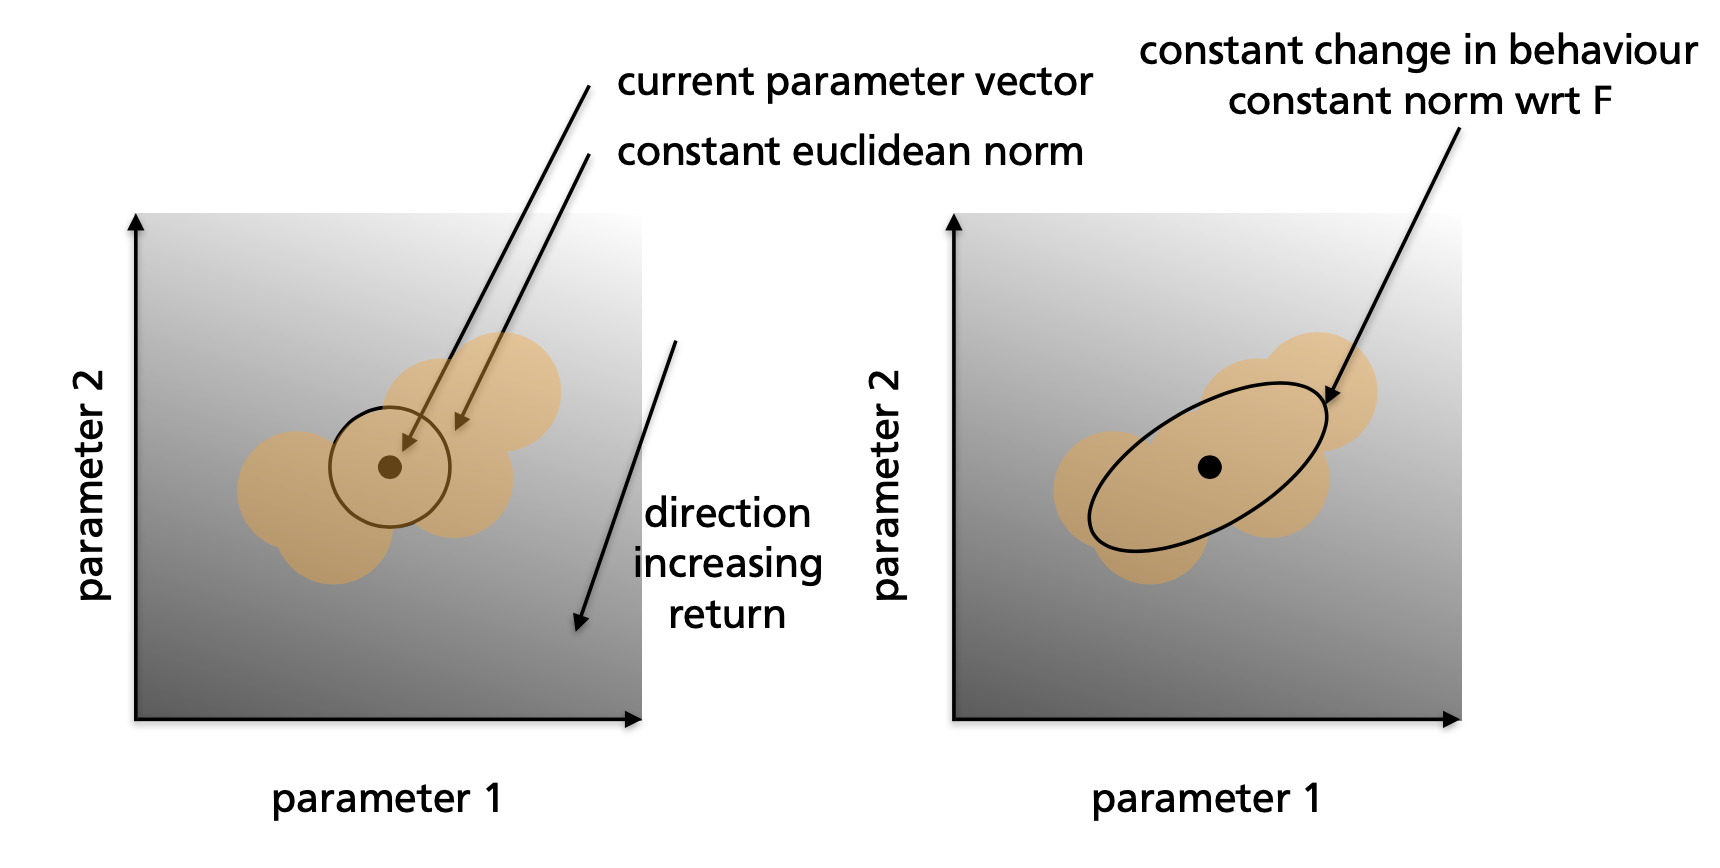
\includegraphics[width=0.5\textwidth]{figures/rl_policy_gradients_NPG.png}
		\caption{Comparison of L2 norm update (left) and NPG (right). The orange background represents the safe changes, meaning the parameter changes for which our policy does not change greater than our defined threshold. While the L2 sticks with the unit sphere, NPG can represents ellipsoids so that we can take larger steps in parameter space towards increasing $J$ without changing the policy too much.}
		\label{fig:rl_policy_gradients_NPG}
	\end{figure}

	We can also visualize the gradient direction grid, as in Figure~\ref{fig:rl_policy_gradients_NPG_gradient_example}. Gradients that point in the wrong direction, give very slow convergence because we focus on parameters which are already close to optimal. 
	
	\begin{figure}[ht!]
		\centering
		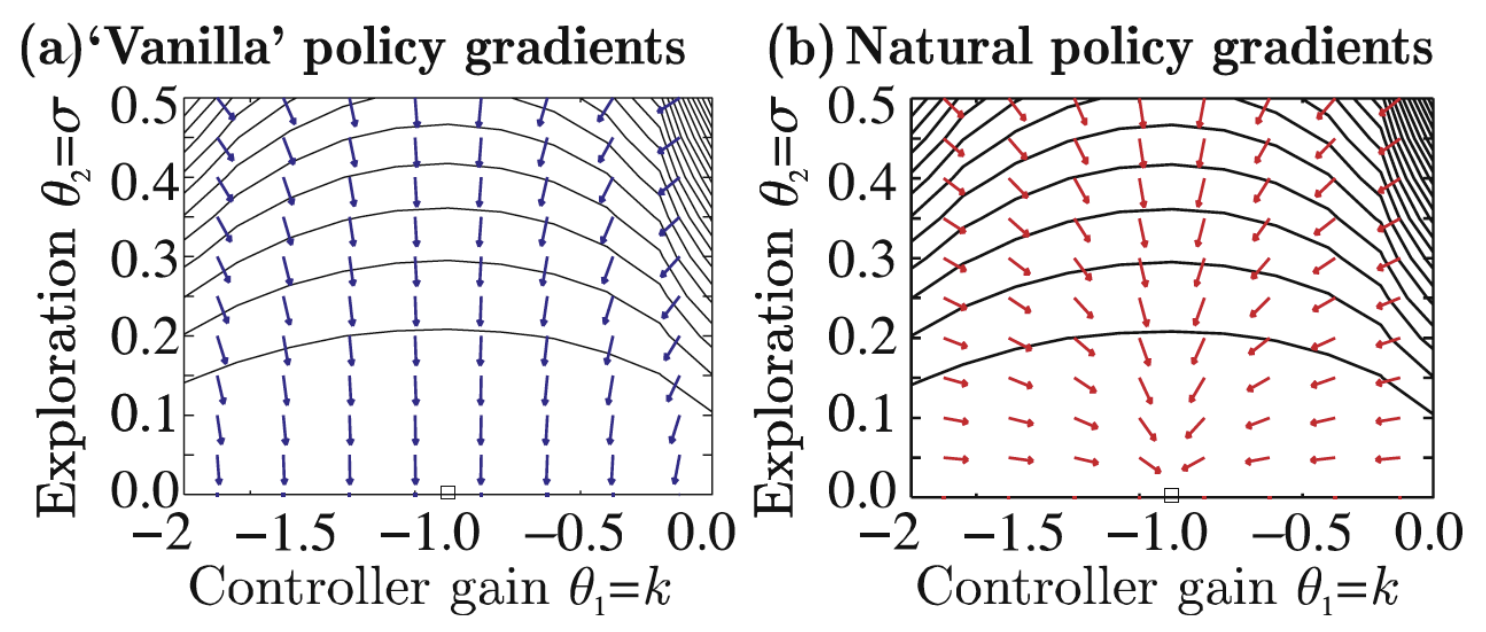
\includegraphics[width=0.4\textwidth]{figures/rl_policy_gradients_NPG_gradient_example.png}
		\caption{Gradient direction over parameter space for finding the optimum at $(-1,0)$. While the NPG gives very smooth transitions, vanilla gradients point straight down (strong gradient for $\theta_2$) for points like $(-2,0.1)$ where we clearly need to update $\theta_1$ more. This leads to slow convergence.}
		\label{fig:rl_policy_gradients_NPG_gradient_example}
	\end{figure}
	\item The advantages of NPG are therefore:
	\begin{itemize}
		\item Faster convergence and less training time
		\item Is an adaptation on top of standard policy gradient, so we can use any of the previous methods with all additions/tricks we want
	\end{itemize}
	However, the biggest drawback is that we have to calculate the Fisher information matrix, which is known for standard distributions like Gaussians, but might be harder to determine for other cases, especially if we want to use a neural network (can be approximated with conjugate gradient algorithm). It also keeps the disadvantages of the other policy gradient methods, namely high variance and still slower convergence compared to value-based methods.
\end{itemize}
\subsubsection{Trust region policy optimization}
\begin{itemize}
	\item A problem of Natural Policy Gradient is that we approximated the KL divergence by a second-order Taylor expansion. The errors that we introduced there, might cause our initial KL constraint to break meaning that $d\theta^T F d\theta\neq c$
	\item TRPO takes a bit different view on the problem. The main concept of the algorithm is that we take as big steps as long as we can guarantee improvement. Hence, we have three steps:
	\begin{enumerate}
		\item Approximate the return function $J$
		\item Apply a penalty term to yield lower bound on the exact function
		\item Maximize lower bound (which guarantees improvement on exact function) by e.g. SGD again
	\end{enumerate} 
	\item The region where we assume our approximation to be valid, is called \textit{trust region}
	\item Figure~\ref{fig:rl_policy_gradients_TRPO_vs_NPG} compares the ideas of NPG and TRPO visually. NPG takes a linear approximation of $J$ at a point, and limits the step size by approximating the KL divergence. TRPO however designs a lower bound which is strictly lower than the "true" function. It is a combination of an approximation of $J$, and a penalty term for big changes in the policy 
	\begin{figure}[ht!]
		\centering
		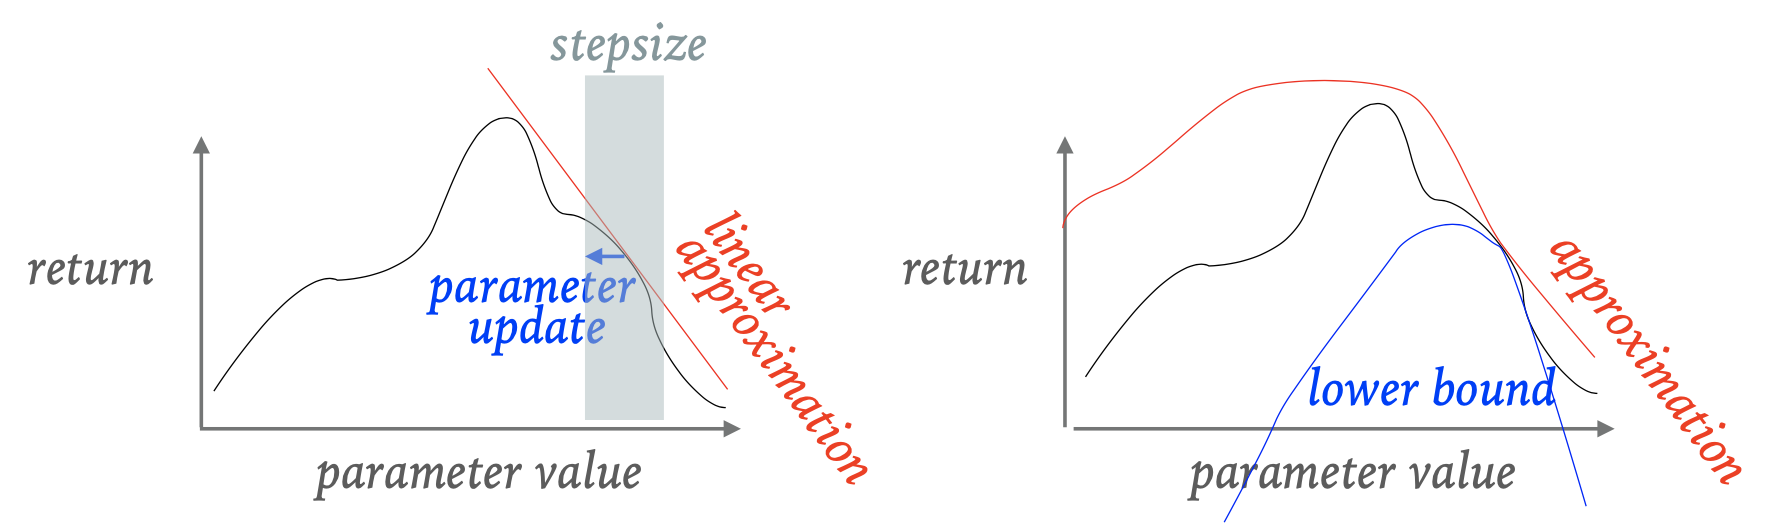
\includegraphics[width=0.55\textwidth]{figures/rl_policy_gradients_TRPO_vs_NPG.png}
		\caption{Comparing the optimization properties of NPG (left) and TRPO (right).}
		\label{fig:rl_policy_gradients_TRPO_vs_NPG}
	\end{figure}
	\item We can calculate the return by:
	$$\eta(\theta)=\E_{\bm{s}\sim \mu_{\pi_{\theta},\bm{a}\sim \pi_{\theta} }(s)}[r(\bm{s},\bm{a})]$$
	where we use samples from $\pi_{\theta}$ to approximate the expectation. However, as soon as we shift $\theta$, we cannot use the same samples anymore because we would be biased. Hence, we can use importance weights:
	$$\eta(\theta)\approx \E_{\bm{s}\sim \mu_{\pi_{\theta}},\bm{a}\sim \pi_{\theta'} (\bm{s})}\left[\frac{\pi_{\theta}(\bm{a}|\bm{s})}{\pi_{\theta'}(\bm{a}|\bm{s})}r(\bm{s},\bm{a})\Bigg\vert \theta' \right]=L_{\theta'}(\theta)$$
	but note that the state distribution is not changed (hence approximation!).
	\item Now, let's consider how we get the lower bound based on our approximation. 
	$$\eta(\theta)\geq L_{\theta'}(\theta) - \frac{2\epsilon \gamma}{(1-\gamma)^2}\cdot \max_s D_{\text{KL}}\left(\pi_{\theta}(\cdot|s)||\pi_{\theta'}(\cdot|s)\right)$$
	where the factor in front of the penalty is environment/policy dependent. 
	\item Although this term above guarantees us a lower bound, in practice, we might run into multiple issues:
	\begin{itemize}
		\item We need to take the maximum KL divergence over all states. However, in environments with many and/or continuous states, this is often not possible. So, we approximate it by taking the average instead.
		\item The penalty is usually very high so that we cannot make big steps. So, the average can already help to reduce the penalty, but we can also consider the KL divergence rather as a constraint than a penalty. This leads us to a similar approach as for NPG
	\end{itemize}
	\item So, what we do instead is maximizing the approximation as in Natural Policy Gradient, but dynamically set the step size based on a maximum KL divergence that we allow between policies. Meaning, we solve the following equation for step size $\beta$:
	$$D_{\text{KL}} \approx \beta^2 d\theta^T F_s d\theta / 2$$
	with $d\theta$ being in the same direction as NPG. One way of (approximately) solving it is by starting with an initial $\beta_0$, and for a couple of steps, increase it if constraint is fulfilled. Otherwise, reduce until we find a valid, sufficiently high $\beta$.
	
	\item In Figure~\ref{fig:rl_policy_gradients_TRPO_vs_NPG}, we now are at the left image again but the step size is adjusted by the KL.
	\item The advantage of TRPO is that we can take bigger steps than the standard NPG, while in theory, having the guarantee of converging. It has been shown to work well with neural controllers where we approximate $F$ by the conjugate gradients. 
	
	The disadvantages are however, that it still requires many steps, and the return is still a Monte Carlo sample (high variance). The guarantee of convergence is actually broken by all the approximations we took.
\end{itemize}

\subsection{Deep Policy Search}
\begin{itemize}
	\item When using deep neural networks for policy search, we might need to consider a few additional tricks because of the high non-linearity of the networks.
	\item To discuss this, we take deterministic policy gradient as an example, and explain the tricks that are used here
\end{itemize}
\subsubsection{Deterministic policy gradients}
\begin{itemize}
	\item All policy gradient methods we have discussed so far considered stochastic policy. However, it is sometimes preferred to learn a deterministic policy (e.g. remember Q-learning)
	\item This means that we will also learn off-policy (behavior policy $b$ with target/actor $\pi$). All other methods were discussed from the on-policy perspective but could be adjusted for off-policy with some minor modifications like importance sampling
	\item When using a different policy for sampling, we change our state distribution from $\mu_{\pi}$ to $\mu_{\beta}$, so that our return is:
	$$J_{\beta}(\pi_{\theta}) = \int_{\mathcal{S}} \mu^{\beta}(s)Q^{\pi}\left(s,\pi_{\theta}(s)\right)ds$$
	In terms of gradients, we end up with:
	$$\nabla_{\theta} J_{\beta}(\pi_{\theta})=\E_{s\sim\mu_{\beta}}\left[\nabla_{\theta}\pi_{\theta}(s)\nabla_a Q^{\pi}(s,a)|a=\pi_{\theta}(s)\right] $$
	Note that this requires $\pi_{\theta}(s)$ to be differentiable, hence returning continuous actions.
	
	Although our samples are slightly off/biased ($\mu_{\beta}$ instead of $\mu_{\pi}$), this is usually not a problem as $\beta$ is chosen to be $\pi$ with some additional noise (like Gaussian).
	\item Our update equations are as follows:
	\begin{equation*}
		\begin{split}
			\text{TD error }\hspace{2mm}\delta_t & = r_t + \gamma Q^{w}\left(s_{t+1}, \pi_{\theta}\left(s_{t+1}\right)\right) - Q^{w}\left(s_{t}, a_t\right)\\
			\text{Update of $Q$ }\hspace{2mm}w_{t+1} & = w_{t} + \alpha_{w}\delta_t \nabla_{w} Q^{w}(s_t,a_t)\\
			\text{Update of $\pi$ }\hspace{2mm}\theta_{t+1} & = \theta_{t} + \alpha_{\theta} \nabla_{\theta} \pi_{\theta}(s_t) \nabla_{a} Q^{w}(s_t,a_t)|_{a=\pi_{\theta}(s)}
		\end{split}
	\end{equation*}
	where we illustrate the gradients in Figure~\ref{fig:rl_policy_gradients_DPG}.
	\begin{figure}[ht!]
		\centering
		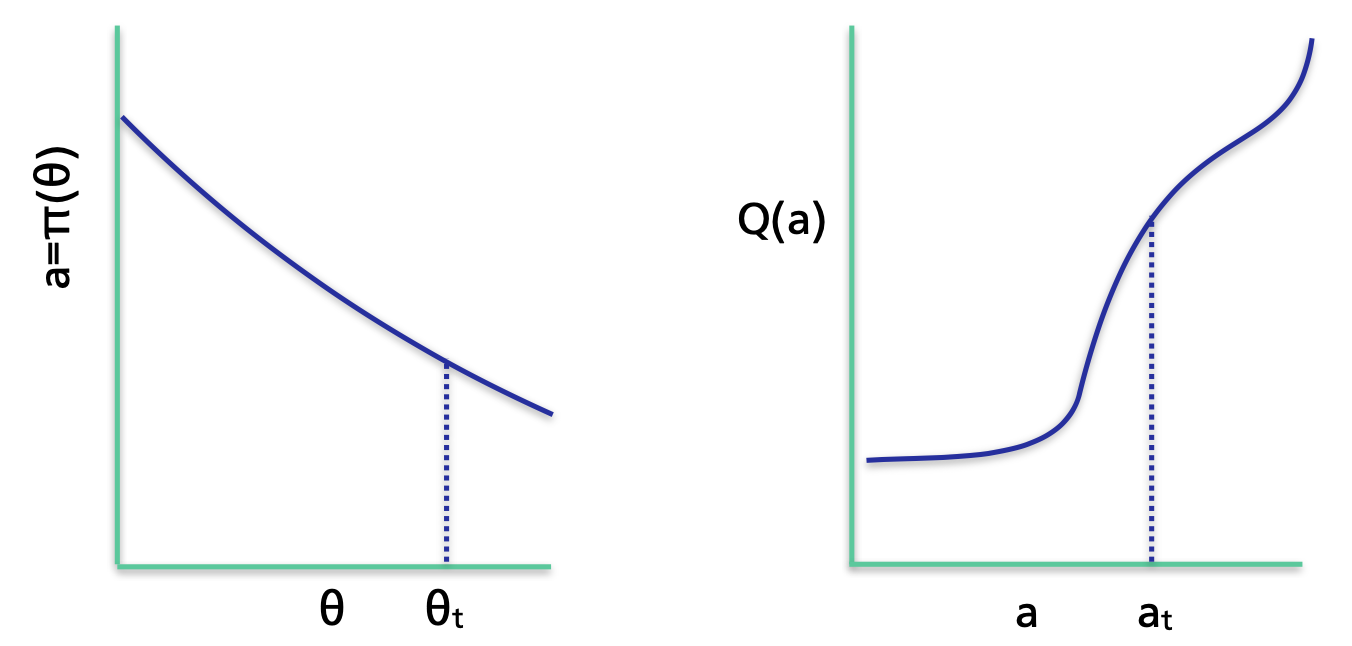
\includegraphics[width=0.5\textwidth]{figures/rl_policy_gradients_DPG.png}
		\caption{Illustrating the gradients in DPG. We have the combination of how much we change the action by changing $\theta$, and how this action change influences the action value $Q^{\pi}$.}
		\label{fig:rl_policy_gradients_DPG}
	\end{figure}
\end{itemize}
\subsubsection{Deep DPG}
\begin{itemize}
	\item When using neural networks, we again have to consider the same issues as in the DQN approach
	\item To use the collected data more efficiently and break the dependency between elements in a batch, we apply \textit{experience replay}
	\item For stabilizing the TD updates, we don't fix the target network, but create a second one that slowly tracks the learned $Q$ values
	\item For ensuring a similar scale of features, we apply \textit{batch normalization} within the network
	\item One aspect of exploration that we have discussed in PGPE before is that independent noise on the actions do not explore well. As a simple improvement, the Deep DPG paper correlates the noise by endorsing to use the same random decision as the time step before
\end{itemize}
\subsection{Summary}
\begin{itemize}
	\item To wrap up policy-based reinforcement learning, we want to put all discussed algorithms into perspective.
	
	\begin{figure}[ht!]
		\centering
		\begin{subfigure}{0.45\textwidth}
			\centering
			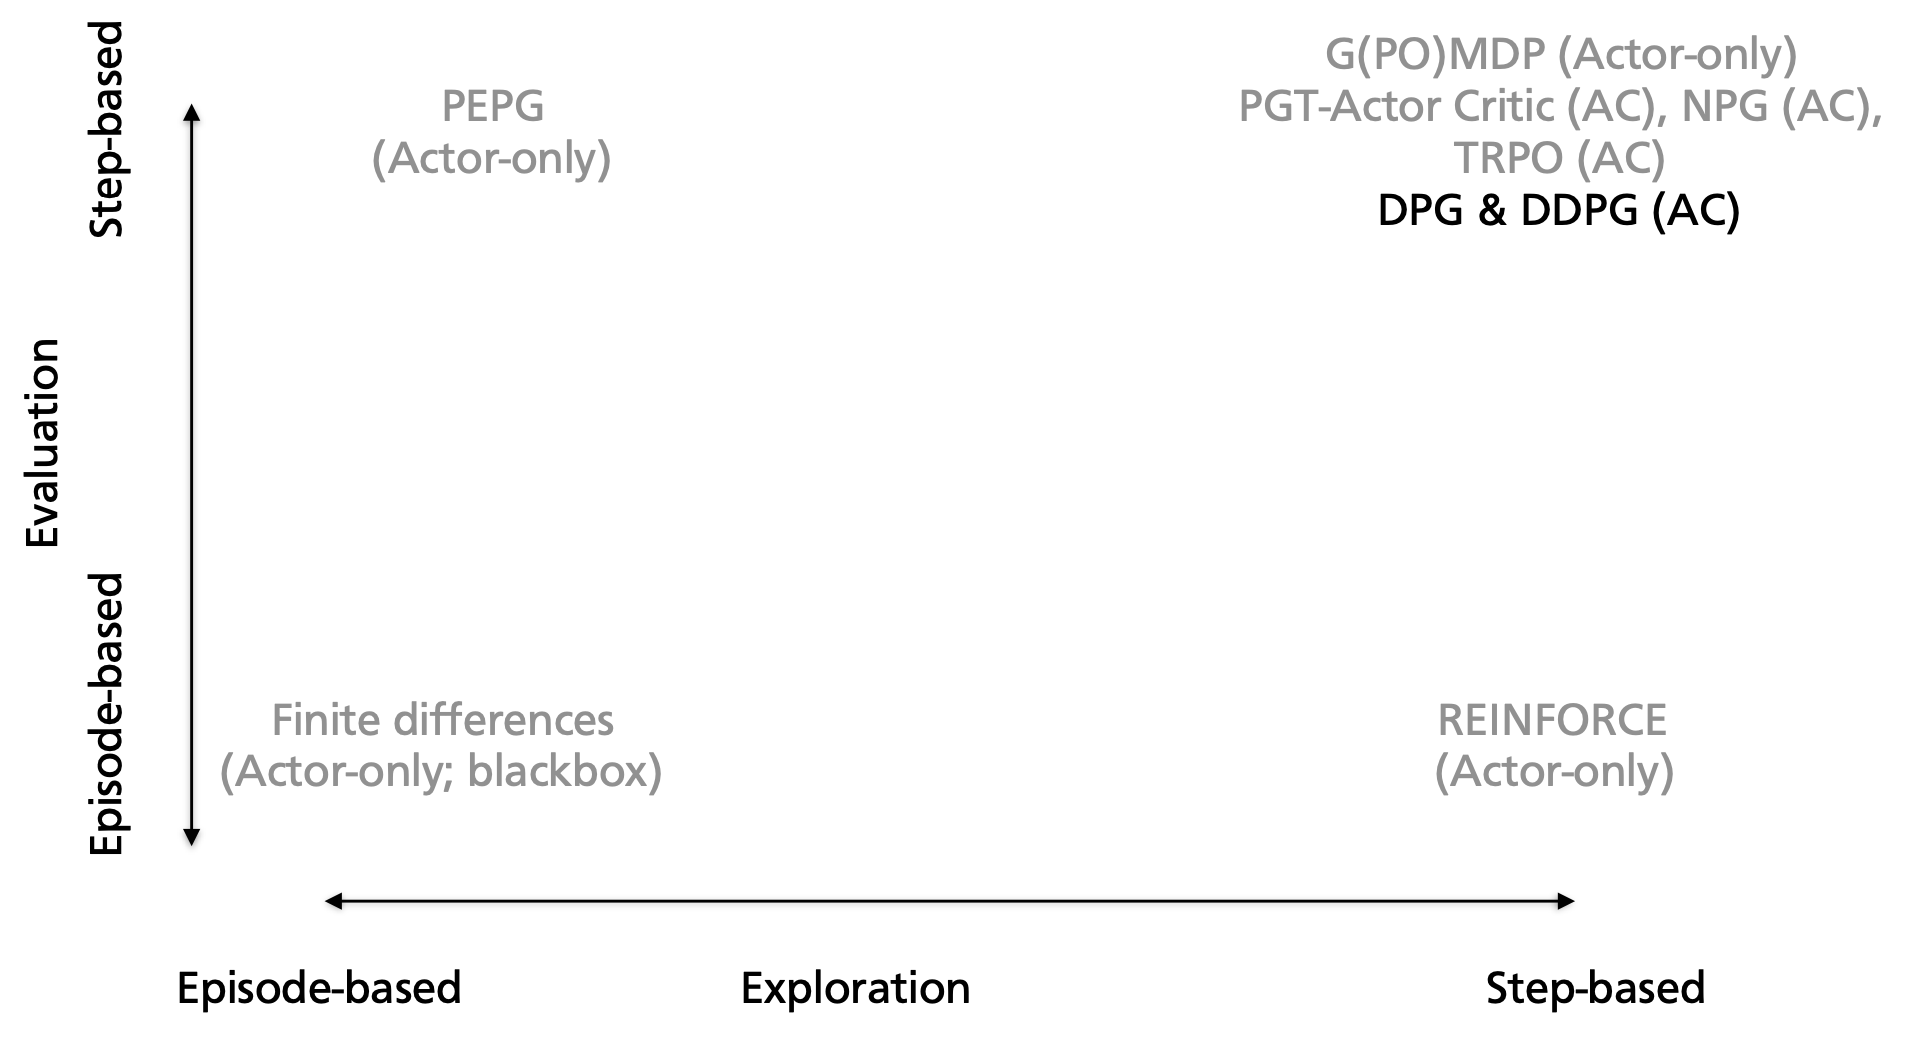
\includegraphics[width=\textwidth]{figures/rl_policy_gradient_summary_1.png}
			\caption{Exploration vs Evaluation}
		\end{subfigure}
		\hspace{5mm}
		\begin{subfigure}{0.45\textwidth}
			\centering
			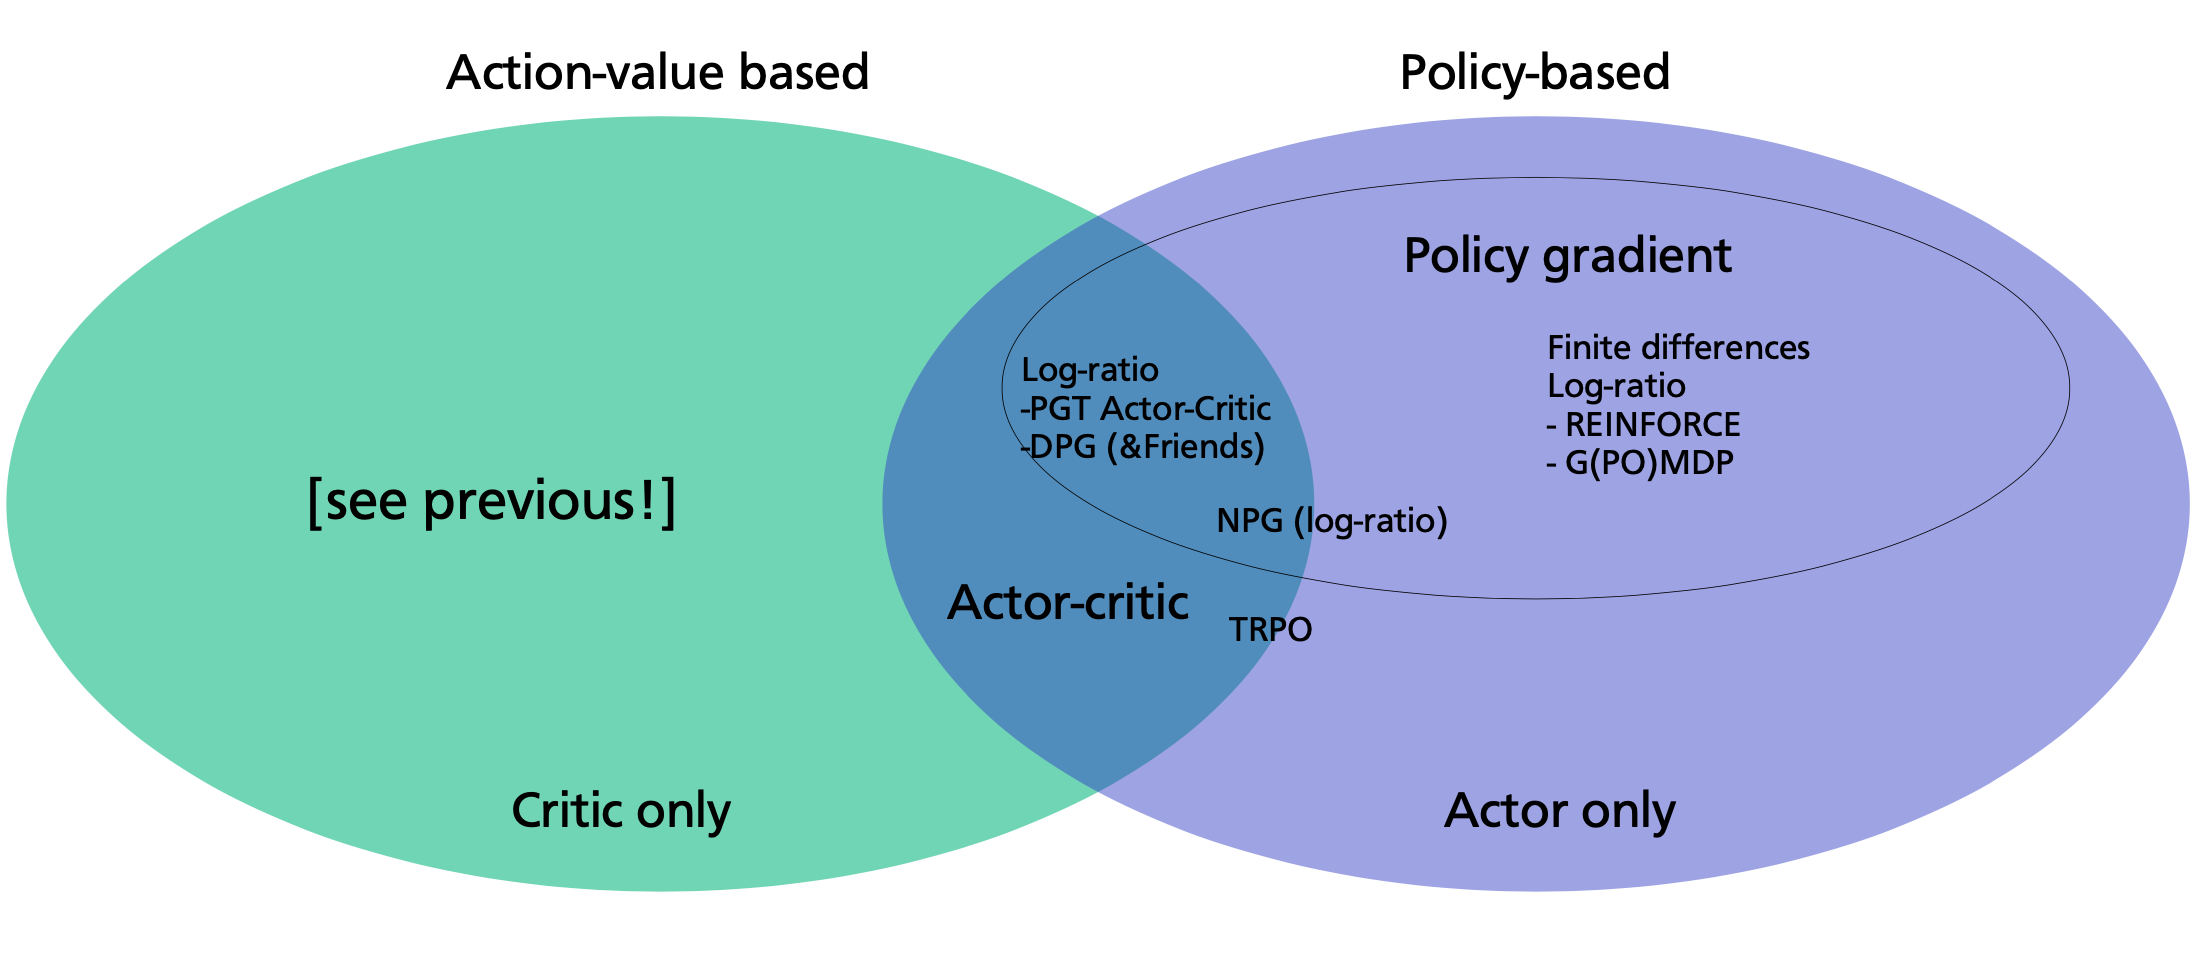
\includegraphics[width=\textwidth]{figures/rl_policy_gradient_summary_2.png}
			\caption{Actor-only versus Value-only methods}
		\end{subfigure}
		\caption{Comparing algorithms across two dimensions. (a) Pointing out the main difference between simple methods and advanced policy gradients (see text for more explanation). (b) Setting policy gradient methods into perspective with value-based.}
	\end{figure}

	\item When discussing the first algorithms of policy gradient, we could distinguish the methods on two dimensions:
	\begin{itemize}
		\item \textit{Exploration}: One key point in the discussion of PGPE was the exploration. Methods like REINFORCE explore by sampling an action at each time step independently, hence their exploration is step-based. PGPE however samples a new policy once in the beginning. This is episode-based because within the episode, we follow a deterministic policy and do not add noise per step. DDPG can be considered as in-between because it adds noise correlations between steps, and hence has not a purely step-based exploration strategy anymore. 
		
		In general, it is hard to say which of both is preferred, and possibly depends on the environment. Independent noise as in the step-based methods have been shown to explore worse (which is why DDPG added the correlation). However, PGPE is more complex to implement and to learn because we have to learn a distribution over parameters $\theta$ which do not one-to-one correspond to distribution over different policies (as discussed in NPG, relation between $\theta$ and $\pi$ might be quite complex).
		
		\item \textit{Evaluation}: Across our discussion, we have seen that some algorithms evaluate their actions step-wise and others per episode. We prefer methods that we can evaluate step-wise because they usually don't need a full sample until the end of an episode (except GPOMDP and other non-Actor-Critic methods), and give every step individual credit assignment. REINFORCE performs episode-based evaluations because the first steps reward influences the last steps update (which we tried to prevent in the other algorithms)
	\end{itemize}
	\item Another part is to consider the different sub-groups of policy-based methods with respect to value-based techniques. REINFORCE, G(PO)MDP and PGPE are all actor-only methods, meaning that they only learn a policy $\pi$. We have seen that we can extend most approaches by introducing a critic that learns $q_{\pi}(s,a)$.
	
	NPG and TRPO can be applied whether with or without actor-critic. Furthermore, we are free to choose how we arrive at $\nabla J$, but note that in the theoretical motivation of TRPO, we use the lower bound so that it is, strictly speaking, not a policy gradient method
\end{itemize}
\newpage 
\section{Model-based Reinforcement Learning}
\label{sec:model_based}
\textit{This section reviews the lecture slides 11 and 12.}
\begin{itemize}
	\item We have seen that given the environment dynamics, we can find the optimal policy by dynamical programming. All the methods after that purely learned from interactions. We now want to take a step in between and try to learn the model dynamics itself, $p(s'|s,a)r(s,a,s')$. If we have that, we could plan by simulating in our learned model.
	\item There are several benefits of this approach:
	\begin{itemize}
		\item We don't require interactions with the environment, but can generate new data from simulation. This is especially helpful when real-time data is expensive (whether in time, computational resources, etc.) as in real-life robotic systems (takes a long time for a single rollout)
		\item We can obtain probability distributions which tell us how likely we end up in a state when we take a certain action. This can be very helpful in some cases, as e.g. in the (slippery) cliff world example, we would know how likely it is that we actually fall of the cliff even if we take the right action. 
	\end{itemize}
	However, when these things are not required, model-free methods mostly work better and/or are computationally cheaper/simpler. Furthermore, we prevent any bias we might get when our model is inaccurate.
	\item In general, we distinguish between three types of systems we can have that tries to imitate the real environment:
	\begin{itemize}
		\item A \textbf{full} or \textbf{distributional model} is a full description of all transition probabilities and rewards. 
		\item A \textbf{sample} or \textbf{generative model} can be viewed as a black-box simulator, where given any state $s$ and action $a$, it can sample a reward $r_t$ and a next state $s'$.
		\item A \textbf{trajectory} or \textbf{simulation model} can simulate whole episodes, but is not able to start at any state and action. This is for example the case for a physical model where we cannot start with an arbitrary velocity.
	\end{itemize}
	These three models can be seen as generalization steps. The most limited implementation is the trajectory one. If we provide the ability of changing the start state to any arbitrary state, we arrive at the generative model. Adding the probabilities $p(s',r|s,a)$ gives us in the end the distributional model.
	\item There are several ways of implementing this. We will consider here a simple method, called Dyna
\end{itemize}
\subsection{Dyna-Q}
\begin{itemize}
	\item Dyna makes two assumptions of the environment:
	\begin{enumerate}
		\item Our environment is deterministic, meaning that any transition probability are either 1 or 0. 
		\item The state and action space is discrete and limited, so that we can store it in a tabular setting.
	\end{enumerate}
	Note that we can relax the first requirement slightly by storing e.g. how often we came from one state-action pair to another state.
	\begin{figure}[ht!]
		\centering
		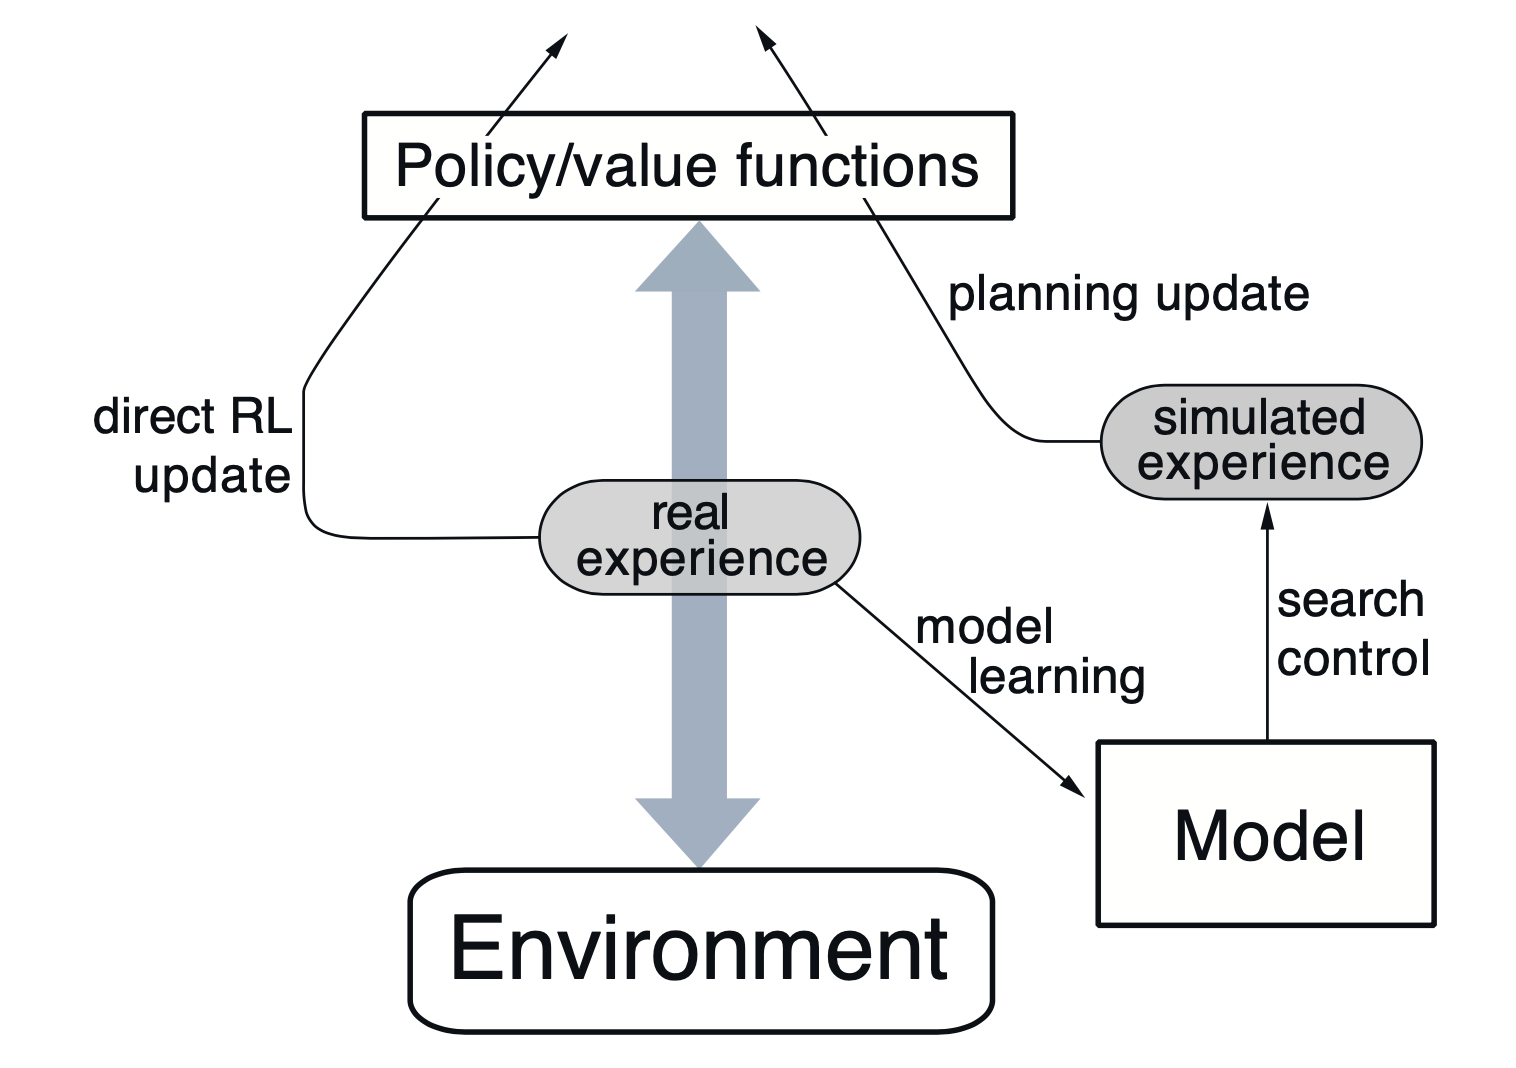
\includegraphics[width=0.4\textwidth]{figures/rl_model_based_dyna_Q.png}
		\caption{Real experience is generated by the interaction of the agent (according to the policy) and the environment. This real data is used to update our policy (direct RL), but at the same time update our model, from which we can generate new samples to learn from (indirect RL).}
		\label{fig:rl_model_based_dyna_Q}
	\end{figure}
	\item The general overview of the idea is shown in Figure~\ref{fig:rl_model_based_dyna_Q}. We have two source from which we train our policy and/or value function: direct and indirect. The samples from the real environment are used to perform "direct Reinforcement Learning" as we use the actual samples to learn. At the same time, we use the real samples to update our model, and can generate from there as many samples as we want.
	\item Written down as an algorithm, we arrive at Figure~\ref{fig:rl_model_based_dyna_Q_algorithm}. The parameter $n$ which specifies how often we train from the simulated/learned model compared to the real environment, is a hyperparameter and depends on the access of the environment (how expensive is it, etc.). However, it is usually $n\gg 1$.
	\begin{figure}[ht!]
		\centering
		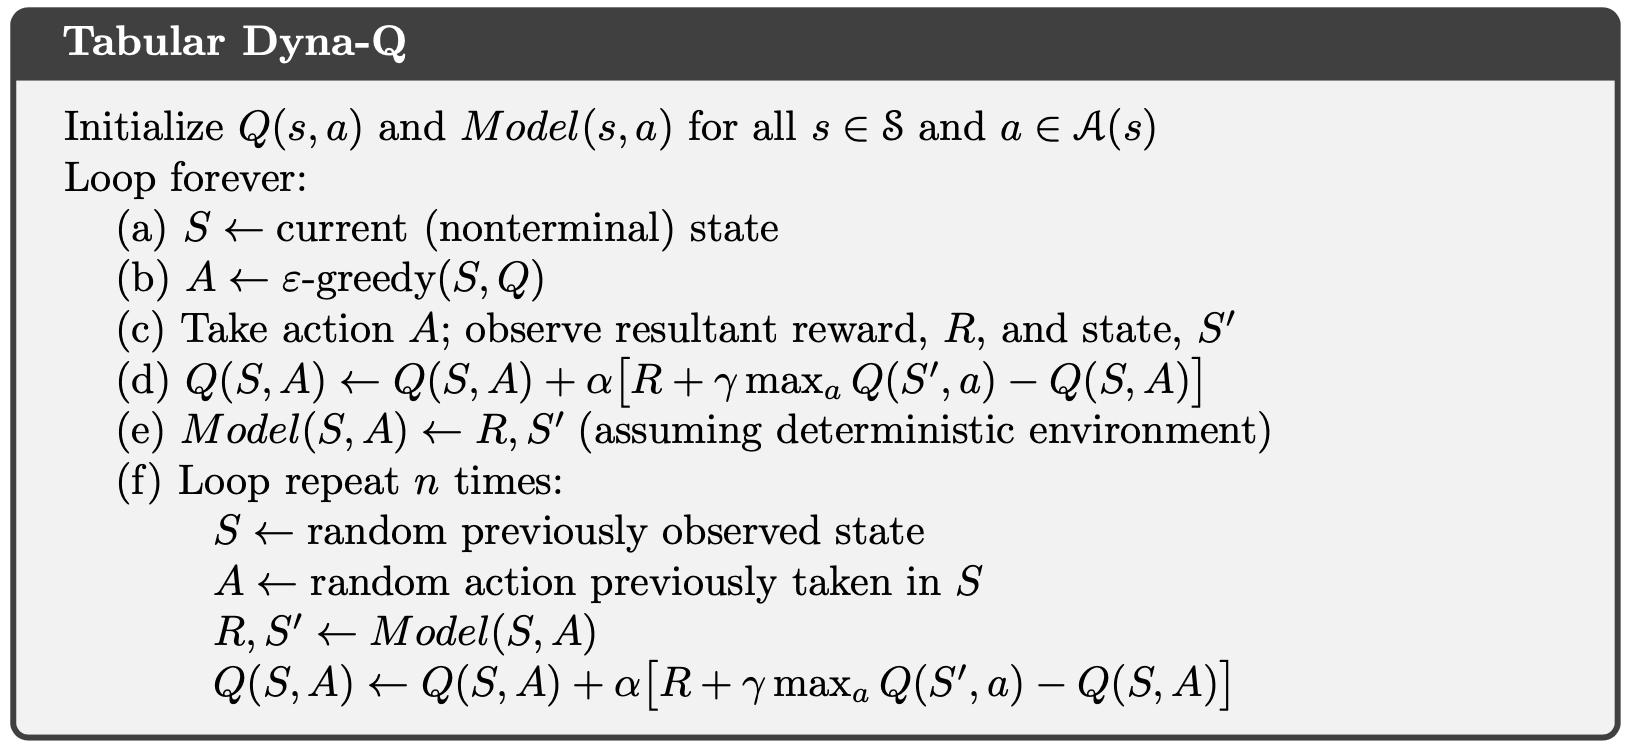
\includegraphics[width=0.65\textwidth]{figures/rl_model_based_dyna_Q_algorithm.png}
		\caption{Example implementation of the algorithm of Dyna-Q. We use a tabular-based setting to store transition and rewards. Note that we will discuss the design choices in this part more in detail.}
		\label{fig:rl_model_based_dyna_Q_algorithm}
	\end{figure}
	\item Looking at Figure~\ref{fig:rl_model_based_dyna_Q_algorithm}, we see that there are still quite a few design decisions to make, which we will go through step-by-step:
	\begin{enumerate}
		\item Step (e) - How do we learn our model?
		\item Step (f) - When should we use our simulated environment? Can we also use it somewhere else than the update step?
		\item Step (f) loop - Which state and action should we choose to update?
		\item Step (f) loop - How do we update e.g. our values or policy?
	\end{enumerate} 
\end{itemize}
\subsubsection{How to learn the model}
\begin{itemize}
	\item As mentioned previously, Dyna uses a tabular setting to learn the model. Hence, we have a table over state and actions, where an entry contains the information of the next state and reward
	\item In case we have stochastic transitions, we have to slightly adjust our table. We now create a table over $(s,a,s')$ where we store how often we experienced this transition, and what reward we got. In case we also have stochastic rewards, we need to extend the table further.
	
	When sampling, we first have to normalize the probabilities for every $s'$ (and $r$) to occur when $(s,a)$ is given, and finally sample from this distribution.
	
	An example table is shown below
	\begin{table}[ht!]
		\centering
		\begin{tabular}{c|cc}
			& \textit{State 1} & \textit{State 2}\\
			\hline
			\textit{State 1, Action 1} & $\eta_{111}=1, r_{111}=2$ (50\%) & $\eta_{112}=1, r_{112}=-1$ (50\%)\\
			\textit{State 1, Action 2} & $\eta_{121}=5, r_{121}=5$ (100\%) & $\eta_{122}=0, r_{122}=0$ (0\%) \\
			\textit{State 2, Action 1}  & $\eta_{211}=4, r_{211}=-4$ (80\%) & $\eta_{212}=1, r_{212}=2$ (20\%)  \\
			\textit{State 2, Action 2} & $\eta_{221}=4, r_{221}=-2$ (40\%) & $\eta_{222}=6, r_{222}=1$ (60\%) \\
		\end{tabular}
		\caption{Example table for stochastic transitions and deterministic rewards.}
	\end{table}
\end{itemize}
\subsubsection{What to update}
\begin{itemize}
	\item To prevent that we spend too much computational effort on state-action pairs that are not relevant for the current/optimal policy, we should make smarter selections
	\item One approach is \textbf{prioritized sweeping} where we prefer these state-action pairs that lead to a state for which we just have experienced an update (whether with real or simulated experience)
	\begin{itemize}
		\item The priority in the queue is given by the TD error we would get at the time we add the state in the queue. This supports that states with high errors, i.e. wrong estimates, are updated first.
		\item To limit the queue, we can define a threshold $\theta$ over which the TD error has to be to add a state in the queue
		\item In the simulation step (indirect RL), we perform updates based on the queue until either the queue is empty, or we reached a maximum of $n$ steps. If the queue is non-empty, it is kept for next iteration as well.
		\item For this model, we require at least a sample/generative model because we need to be able to start at any state-action pair
		\begin{figure}[ht!]
			\centering
			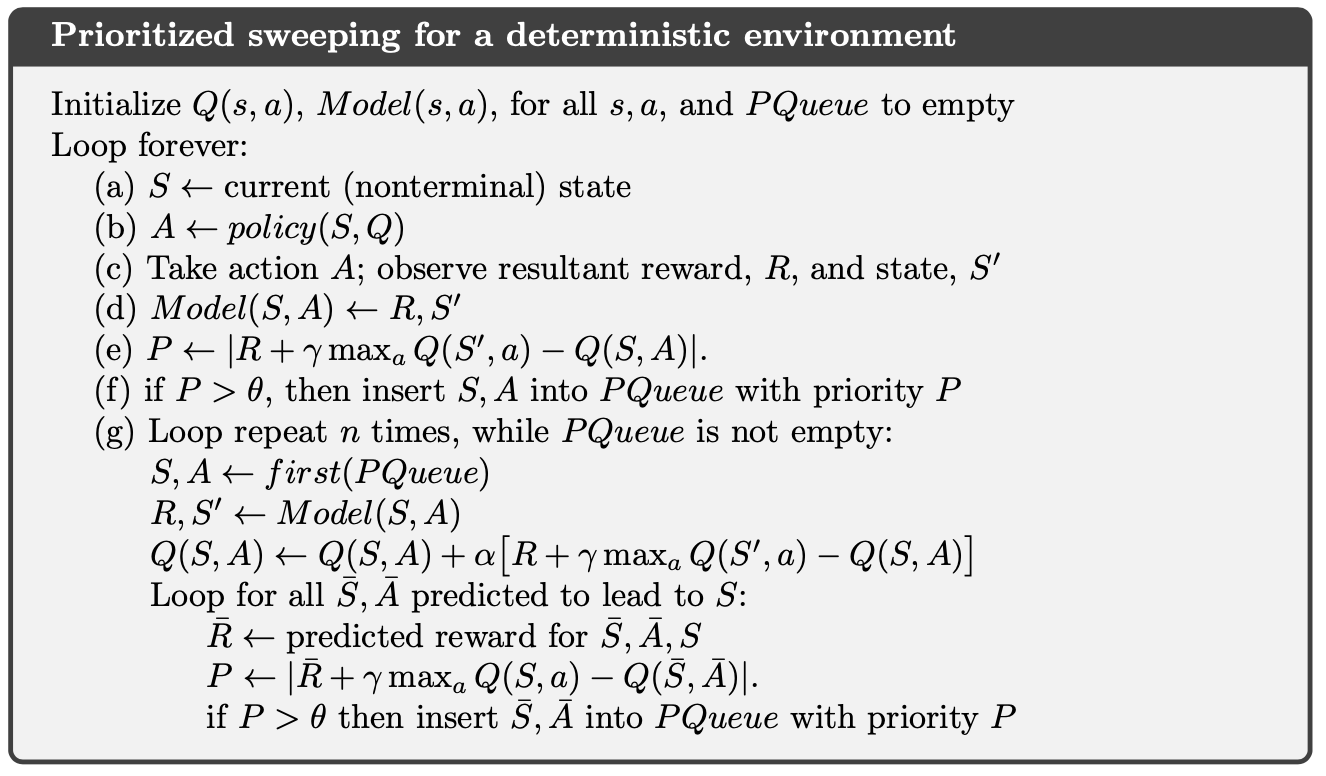
\includegraphics[width=0.5\textwidth]{figures/rl_model_based_dyna_prioritized_sweeping.png}
			\caption{Algorithm of Prioritized Sweeping.}
		\end{figure}
	\end{itemize}
	\item An alternative is performing \textbf{trajectory sampling} where we start from the start state (or sample one if multiple exist), and follow our current policy. 
	\begin{itemize}
		\item While updating the more frequently visited states, we have the disadvantage of limited exploration because we highly focus on states of our distribution
		\item Hence, if we have a (close to) deterministic environment, trajectory sampling might work well, but in a stochastic environment where we continuously have to explore, it might perform worse than uniformly sample any state-action pair 
		\item For this method, we only require a trajectory model, making it less complex
	\end{itemize}
\end{itemize}
\subsubsection{How to update}
\begin{itemize}
	\item For updating our $q$/$v$/policy, we can use any of the methods we have discussed before. 
	\item However, remember that for some methods like dynamic programming, we can make use of the model dynamics. Nevertheless, this might not be the most efficient computation, especially when we have many possible next steps. Remember that we have to take \underline{all} next states into account for dynamic programming, although some can be neglected if we have a small weight on them. 
	\item In addition, we would require the full/distributional model to perform these kind of updates, whereas the others either work with generative or trajectory models
\end{itemize}
\subsubsection{When to plan}
\begin{itemize}
	\item Currently, we only use the environment to generate new samples for training
	\item Knowing the system dynamics can however be valuable in more than this situation. For example, we can easily plan ahead by trying out different actions, and observing the reward in simulation. Afterwards, we take the actions in real-world which gave the best result in the simulation
	\item This idea is used in Monte Carlo Tree Search algorithms, which we will discuss in more detail in Section~\ref{sec:MCTS_Alpha_Go}. 
\end{itemize}
\subsection{Model-based policy search}
\begin{itemize}
	\item In the previous discussion, we mainly focused on value-based updates. However, we could of course use policy-based methods as well.
	\item Again, the decision of whether to use policy-based or value-based methods is based on multiple decisions. For example, if we need to learn a stochastic policy, or we have continuous actions, then we might want to use policy-based methods. In the case that we have discrete actions and aim for learning a deterministic, greedy policy, value-based methods are more suited because for policy gradient we require the policy to be smoothly changable/differentiable.
	\item Let's assume that the reward is known for now (e.g. we have defined the reward for a problem by our own). Then, we could reformulate the transition function as:
	$$s_{t+1} = f(s_t, a_t) + w$$
	where $f(s_t, a_t)$ is a deterministic function that maps a state-action pair to a new state, and $w$ is additive noise (e.g. Gaussian for continuous states). To ensure this formulation to work well, we would require a mostly deterministic environment, as otherwise $f(s_t, a_t)$ cannot model the different outcomes.
	\item We can then train by
	\begin{enumerate}
		\item Use any model-free policy-based approach (e.g. TRPO or DDPG) to learn from the real world.
		\item Use the extra information from the environment, e.g. for richer gradient information
		\begin{itemize}
			\item As we now model the transition function $s_{t+1}\approx f(s_t, a_t)$, we know how the next state will change if we change our parameters.
			\item This allows us to look at the gradients over $s'$ and $a$, and find the best action more easily
			\item When we perform backpropagation through $v_{\theta}(s_t)$, we can (instead of sampling) also derive rewards because they are a simple function depending on $s_{t+1}$, or in $f(s_t,a_t)$. Hence, we can write:
			$v_{\theta}(s_t)=\nabla_{\theta} r_{t+1}+\gamma \nabla_{\theta} r_{t+2}+...$
		\end{itemize}
	\end{enumerate}
\end{itemize}
\subsection{Monte-Carlo Tree Search and Alpha Go}
\label{sec:MCTS_Alpha_Go}
\begin{itemize}
	\item In Section~\ref{sec:value_based_approximation}, we have seen that to learn a value function for problems with very large state space, we can approximate our $q$-function by e.g. a neural network. However, these approximations will always contain a certain amount of noise/inaccuracy.
	\item An alternative approach is to learn $q_{\pi}(s,a)$ \underline{online}. The simplest approach, when we have given our model, is to perform a couple of rollouts from the state $s_t$ with our current policy $\pi$. $q_{\pi}(s,a)$ can then be estimated by the mean of the experienced returns $G_t$.
	
	Playing the best action based on this estimate (e.g. estimated $q_{\pi}(s_t,a_1)$, $q_{\pi}(s_t,a_2)$, etc.) is guaranteed to be at least as good as $a\sim \pi(s)$ as if $\pi$ was the optimal policy, $a$ will also be the argmax of the estimate (in expectation).
\end{itemize}
\subsubsection{Monte-Carlo Tree Search}
\begin{itemize}
	\item If we have given a full model description including the dynamics, we could simply expand the previous approach by taking all possible futures into account. However, this is less likely to work for games like Go because there are a huge number of possible outcomes (a full game tree has about $10^{170}$ different states). 
	\item Nevertheless, a lot of this computation might not be necessary. Instead, we can focus on the most likely subtree which only contains a small selection of possible outcomes. This leads us to the Monte-Carlo Tree Search algorithm
	\item In MCTS, we build a tree incrementally by performing 4 steps for $n$ steps (limited by computational resources, time, etc.), visualized in Figure~\ref{fig:rl_model_based_MCTS}:
	\begin{enumerate}
		\item \textbf{Selection}
		
		Given a subtree, we need to decide at which point we want to expand it. This is defined by our \textit{tree policy} $\pi_{\text{tree}}$, and can be for example the upper confidence bound (similarly to choosing the next action in a bandit setting):
		$$\pi_{\text{tree}}(s)=\arg\max_{a} \left[Q(s,a)+c\sqrt{\frac{\ln N(s)}{N(s,a)}}\right]$$
		with $N(s)$ as the number of visits in $s$, and $N(s,a)$ the number of times we took $a$ in $s$. We continue our policy until we end up at a leaf node.
		\item \textbf{Expansion}
		
		After deciding at which node we want to "grow" the tree, we need to expand it. This means that we add a new leaf, which is an action in case of $q$, or a state in case of $v$ (we always add a state-action pair, just ordering is different). We initialize it with the values $N(s)=0$, $N(s,a)=0$ in case of UCB.
		\item \textbf{Simulation}
		
		From the newly added node, we perform a rollout. This means that starting from the leaf node, we interact with the environment according to the current policy $\pi$ until terminating. 
		\item \textbf{Backup}
		
		After finishing simulation, we update our estimates based on the newly observed return. Note that we update the $q$/$v$-values for each node which led to the leaf, while taking a possible discount factor $\gamma$ into account. In case of UCB, this means that we increase $N(s)$ and $N(s,a)$ by one, as well as adding a new point to $Q$ for averaging (e.g. use running average).
	\end{enumerate}
	\begin{figure}[ht!]
		\centering
		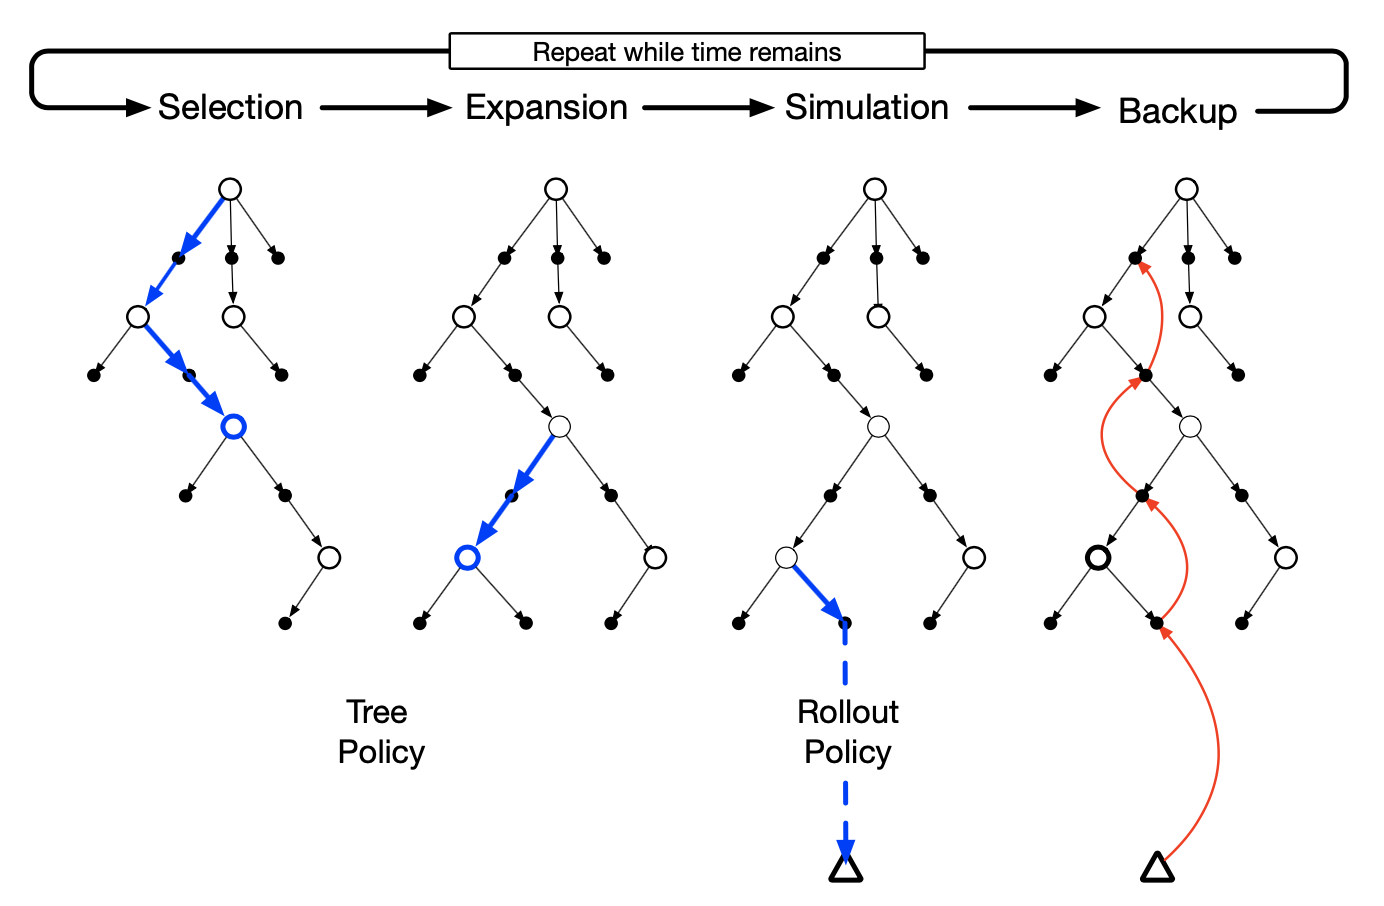
\includegraphics[width=0.6\textwidth]{figures/rl_model_based_MCTS.png}
		\caption{Visualization of the four steps in MCTS: Selection, Expansion, Simulation, Backup.}
		\label{fig:rl_model_based_MCTS}
	\end{figure}
	\item Note that we have seen two requirements of MCTS along the way: (1) we need a generative model where we can start at any $(s,a)$. Alternatively, if our environment is deterministic, we can also make trajectory models working by playing the same actions again from the top. (2) we assume $q(s,a)$ to be storable in a table
	\item If we want to use MCTS for planning, we can choose our our policy based on $\pi(a|s)\propto N(s,a)^{1/\tau}$. Note that we don't take the policy according to the $q$ values because they are estimates, and potentially very noisy as we have different amount of samples for each action.
	\item After taking a step, we can reuse the selected branch of the tree, and don't have to start from scratch again
\end{itemize}
\subsubsection{AlphaGo Zero}
\begin{itemize}
	\item For estimating the $q$-values, MCTS uses full Monte Carlo samples. However, we know that we can also use TD learning for it, meaning we bootstrap our estimates. Using this idea, two separate networks were used in Alpha Go: a policy network $\pi_{\theta}(a|s)$, and a value network $v_{\theta}(s)$
	\item We can now look at the changes AlphaGo makes in the MCTS algorithm:
	\begin{enumerate}
		\item \textbf{Selection}
		
		We define our tree policy as:
		$$\pi_{\text{tree}}(a|s)=\arg\max_a \left[Q(s,a)+cU(s,a)\right], \hspace{5mm}U(s,a)=\frac{\pi_{\theta}(a|s)}{1+N(s,a)}$$
		Note that this is a solution found empirically as we sum $q$-values and probabilities.
		
		\item \textbf{Expansion}
		
		When reaching a leaf node, we evaluate the value network $v_{\theta}(s)$ for this specific state, and expand the state by all its possible actions.
		
		\item \textbf{Simulation}
		
		In the original AlphaGo, we randomly choose between using $v_{\theta}(s)$, or simulating by performing a rollout. However, in the newer version AlphaGo zero, we fully rely on $v_{\theta}(s)$.
		
		\item \textbf{Backup}
		
		Using $v_{\theta}(s)$, we update all $q$ values above.
	\end{enumerate}  
	\item Our policy network $\pi_{\theta}$ limits our search in width because we select values based on its prior. The value network $v_{\theta}(s)$ limits the search in depth because we don't have to sample anymore.
	\item This approach is working well, if we have (1) a discrete state space, (2) a fully observable environment, and (3) a deterministic environment.
	\item We train the network by self-play. The policy network tries to predict the outcome of the tree search (how often will we choose action $a$ at state $s$), and the value network tries to predict the return we get after the full rollout. See Figure~\ref{fig:rl_model_based_alphago_zero_selfplay} for a visualization of the self-play learning.
	\begin{figure}[ht!]
		\centering
		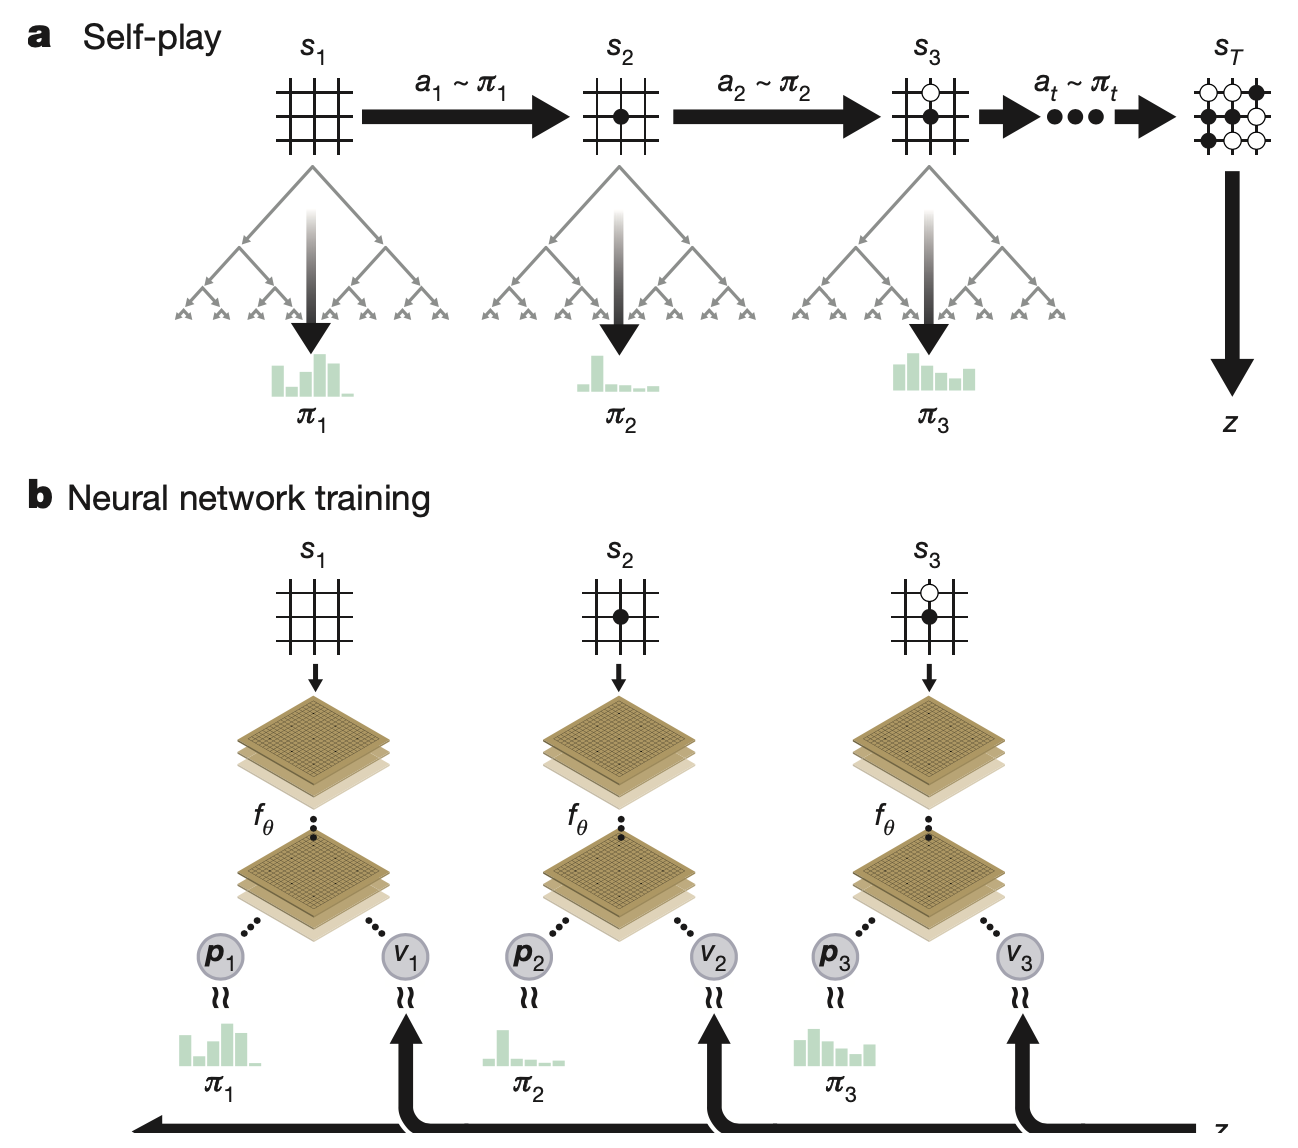
\includegraphics[width=0.4\textwidth]{figures/rl_model_based_alphago_zero_selfplay.png}
		\caption{Self-play RL in AlphaGo zero.}
		\label{fig:rl_model_based_alphago_zero_selfplay}
	\end{figure}
	\item Nevertheless, the training might not be 100\% stable. In a small amount of times, it can happen that the network diverges. To prevent this, we evaluate the network every $n$ steps by playing against itself/an older version of itself. If the policy did not improve (i.e. loosing more games than winning against older version), we throw away the new model and start again from the old weights. 
\end{itemize}
\newpage
\section{Partially observable environments and Bayesian methods}
\label{sec:partially_observable}
\textit{This section reviews the lecture slides 13.}
\begin{itemize}
	\item Until now, we always assumed to have a fully observable environment. However, this is often not the case, also in real life (we cannot see what is happening behind walls, or 1000km away. Thus we are \textit{living} in a partially observable environment).
	
	This can happen if we have state aliasing (we see twice the same state although if it would be fully observed, it is clear that we are in two different states), or even simple noise.
	\item First, let's consider a generalization of our environment. We define a latent state in the environment $x'_t$ which captures all information about the true state. From this latent state, we can make an observation $o_t$ per state, which can be seen as measurement of an unknown quantity.
	
	Note that in fully observable environments, we have $s_t=o_t=x'_t$.
	\item A simple approach would be to consider an observation $o_t$ as features from the latent state, and hence use approaches from Section~\ref{sec:value_based_approximation}. But this is usually not sufficient.
	\item In most environments, we can infer information about the latent space by looking at the history $H_t=A_0,O_1,A_1,...,A_{t-1},O_t$, and we choose our next action based on the whole history $A_t=\pi(H_t)$
	\item However, using a full history is neither efficient nor practical (increases in size over time). Hence, we better use a lower dimensional feature representation of the history, $f(H_t)$, and use this as internal state of the policy $s_t = f(H_t)$ (note that $s_t$ has slightly different meaning here because it is the state which the policy sees, not what we get back from the environment).
	\item The best function $f$ would be the one that summarizes all important information. We can define what this means as follows:
	$$f(H_t)=f(H'_t)\implies \Prob{O_{t+1}=o|H=H_t,A_t=a}=\Prob{O_{t+1}=o|H=H'_t,A_t=a}$$
	which means in textual form: if the representation of two histories are the same, then the expectation of the next observation is the same for both histories. Hence, we would also choose the same action, which leads to the conclusion, that the optimal policy can be found solely on $f$.
	
	A function that fulfills this condition is called \textit{Markov function}. For any function which is not Markov, we can only find an approximate optimal policy, but often not the optimal itself.
	\item Which function is Markov depends highly on the environment, and will be discussed next.
\end{itemize}
\subsection{Markov functions and histories}
\begin{itemize}
	\item First, let's consider what we need to deal with a partially observable environment. Besides the environment and our policy-/value-based approach, we also have a state-update function (see Figure~\ref{fig:rl_partially_observability_architecture}). Our goal is to find a state-update function which is Markov and efficient/compact.
	
	\begin{figure}[ht!]
		\centering
		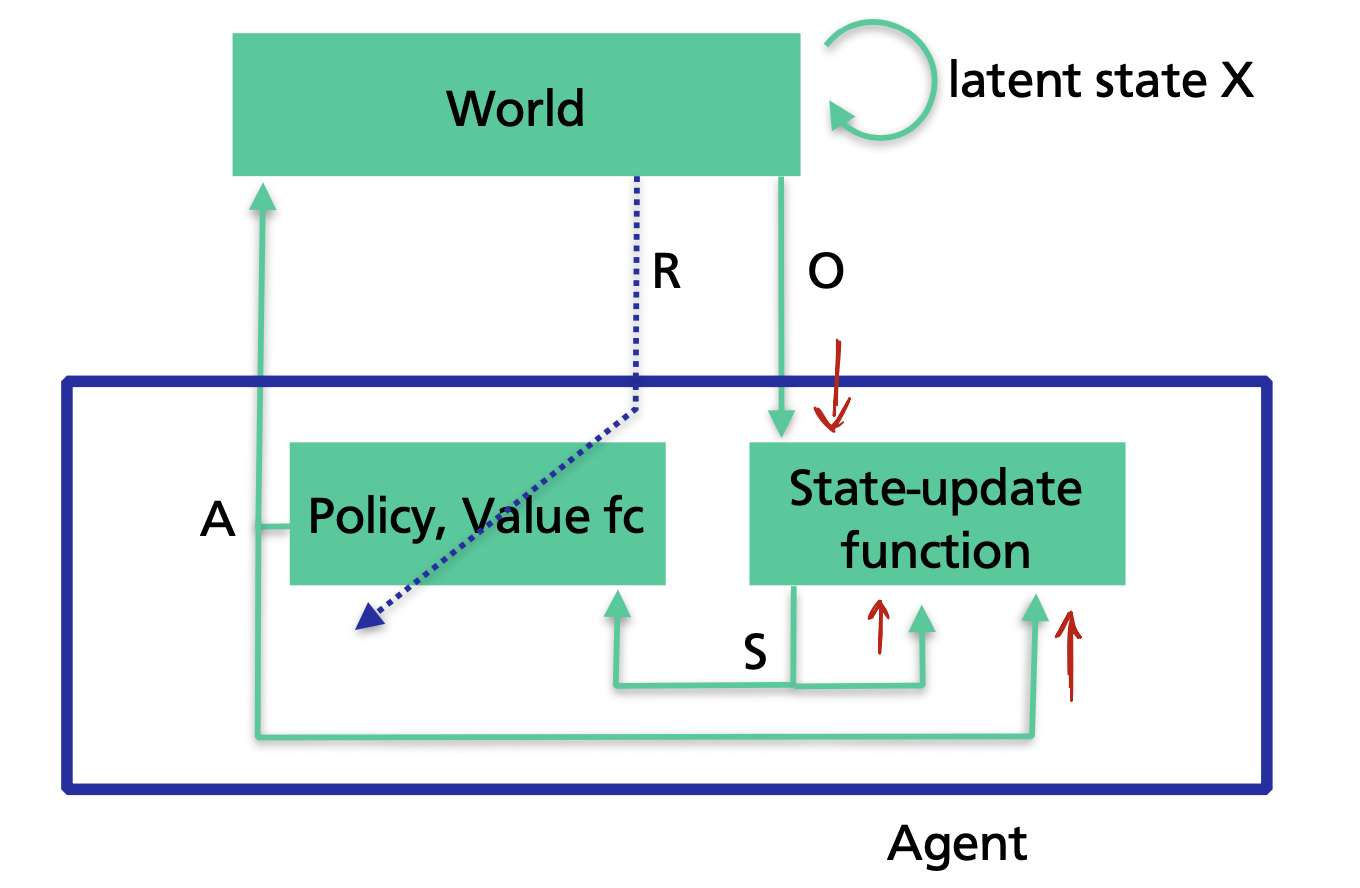
\includegraphics[width=0.5\textwidth]{figures/rl_partially_observability_architecture.png}
		\caption{Overview of the dynamics in dealing with a partially observable environment.}
		\label{fig:rl_partially_observability_architecture}
	\end{figure}
\end{itemize}
\subsubsection{Sample Markov functions}
\begin{itemize}
	\item The simplest function is the identity, meaning $s_t=H_t$. However, this is neither compact, nor can we use it in any tabular policy setting efficiently (all possible sequences must be stored).
	\item We can define an probability distribution over the latent space $X$, and try to do Bayesian inference (i.e. finding the posterior). This is done by calculating a \textbf{belief state}:
	\begin{equation*}
		\begin{split}
			s'(x)=p(x'|o',a,s)& =\frac{p(o'|x',a,s)p(x'|a,s)}{p(o'|a,s)}\\
			& = \frac{p(o'|x',a)p(x'|a,s)}{p(o'|a,s)}\hspace{5mm}\text{(removing $s$ as $x'$ is given as true state)}\\
			& = \frac{p(o'|a,x')\overbrace{\sum_x p(x'|x,a)s(x)}^{=p(x'|a,s)}}{\sum_{x'}p(o'|a,x')\sum_x p(x'|x,a)s(x)}
		\end{split}
	\end{equation*}
	where $s(x)$ is the old belief (i.e. belief over $x$ from last step). We can further define $p(o'|a,x')$ as the \underline{observation model} (i.e. what do I see from the latent space), and $p(x'|x,a)$ as the \underline{transition model} (i.e. how likely is it to move from one latent state the another). If we know these model dynamics by a full model description (or can estimate them), we have as state the probability distribution over latent state $x$.
	
	This method is the classical approach for POMDPs, as it is compact, can be updated recursively and is easily interpretable by a human. However, the disadvantages are that we need the underlying model (not always given), and that it is only feasible for a discrete latent state (otherwise sums become integrals etc.).
	\item As last example, we can consider the obvious approach of determining all the observation probabilities:
	$$f(h)=\begin{bmatrix}
	f_{o_1a_1}(h)\\ f_{o_1a_2}(h)\\\vdots\\f_{o_2a_1}(h)\\\vdots\\
	\end{bmatrix}\hspace{5mm}\text{where}\hspace{5mm}f_{oa}(h)=\Prob{O_{t+1}=o|H=h,A_t=a}$$
	Given enough data, we can learn this distribution. Furthermore, we can extend this to longer trajectories like $\tau=a_0o_1a_1o_2a_2o_3$, and it can be proven that for a special set of "core tests" $\tau_1,\tau_2,...,\tau_d$, we can create a Markov state. This is called a \textbf{predictive state representation}.
	
	The advantage is that it is as compact or even more than the belief states as we only have a probability over observations and not the latent space. However, it might be harder to interpret as we only have the probabilities of the "core tests", and it is still limited to the tabular setting.
\end{itemize}
\subsubsection{Approximations with non-Markov functions}
\begin{itemize}
	\item Alternatively, we can also consider non-Markov functions which cannot guarantee to find the optimal policy, but at least an approximate one
	\item The simplest method here is just using the last state, $S_t=O_t$. However, this might not contain all the information we need (e.g. in Atari games, movement cannot be captured), and is often not compact (still have the whole screen)
	
	A slight improvement is stacking a few observations, as in Atari games. This allows us to observe movement, but we still loose long-term dependencies.
	\item We can also apply RNNs which take $O_t$ and $A_t$ as input including the last state $S_{t-1}$, and generate a new state $S_t$. This feature extractor can be learned end-to-end, and applied to a wide range of environments. However, the training might be a bit tricky in terms of hyperparameter tuning. 
\end{itemize}

\subsection{Partial observability and exploration}
\begin{itemize}
	\item We have seen that Markov functions rely on uncertainty of the latent state, which can be consider as trying to take the actions that make you most certain about the latent state (while maximizing the reward).
	\item Hence, we can also consider this as a exploration strategy. If we consider knowledge about our environment which is the set of states and action, we can try to learn the transition probabilities as well by adding them to our state. This leads us to a \textit{hyperstate}:
	$$x_{\text{POMDP}} = (s_{\text{MDP}}, \text{transition}, \text{rewards})$$
	where we consider a fully observable environment as partially observable by adding the transition and reward distributions. Now, we can simply apply POMDP techniques as we have discussed before.
	\item For example, consider a simple environment with 2 states and 2 actions each. Our transition probabilities can be defined as a vector:
	$$p=(p_{11},p_{12},p_{21},p_{22})$$
	where for a prior, we assume a uniform distribution. By interaction, we change our belief towards what we have observed.
	\item Now, an optimal policy will take the uncertainty of the transition probabilities in account, and tries to maximizes the expected return. This leads to an optimal trade-off between exploration and exploitation.
	\item However, keep in mind that we have $|\mathcal{S}|^{|\mathcal{A}|}$ transition probabilities to learn, which can be too large for certain environments. Hence, we might have to consider using approximations again.
\end{itemize}
\subsubsection{Bayesian Adaptive MDP and Meta-reinforcement learning}
\begin{itemize}
	\item Our approach on partial observability can be seen as Bayesian because we use our posterior to estimate the expected reward given a prior of our beliefs (iterative posterior update)
	\item If the prior assigns a non-zero probability to a certain model, then it can find the optimal strategy for it. The amount of samples needed, i.e. exploration, is based on the design of the prior. The closer the prior to a certain model, the less it will have to explore. But giving a model a higher chance in the prior than it should leads also to worse performance on other MDPs.
	\item We can show that to find the optimal strategy for finding the best policy in a unknown MDP can be learned by sampling from the prior over MDPs, and use simple gradient estimates
	\item Hence, with a prior over MDPs, optimal exploration can be phrased as greedy behaviour in an augmented MDP, where the hyperstates include the unknown transition and reward probabilities
	\item Such techniques are investigated under the term \textbf{Meta-reinforcement learning}. Here the agent is not told which exact MDP it gets, but has to learn patterns across MDPs, and find the optimal way of exploring.
\end{itemize}
\newpage
\appendix
\newpage
\section{Deep RL in practice}
\textit{This section reviews the lecture slides 10 (last half).}
\begin{itemize}
	\item There are several things to keep in mind when performing experiments in RL in practice
	\item If we have a research questions that we want to investigate, we need to design experiments for which we have to answer the following questions:
\end{itemize}
\begin{description}
	\item[On which tasks?] We need to find environments which fit to the research question in mind. Things to consider are:
	\begin{itemize}
		\item Continuous control tasks lend themselves to actor critic methods
		\item Pixel-based task can show whether complex input data can be handled
		\item Highly complex tasks show whether a method scales with having lots of compute and training data available
		\item Toy examples can point out difference between methods, so it is often good to have both a toy example, and a more complex, practical one
	\end{itemize}
	\item[Which parameters and architectures to test?] RL have been shown to be very sensitive to the selection of hyperparameters. Hence, you should also spend similar tuning efforts an \underline{all} your experiments, including the baseline, to ensure a fair comparison.
	\item[Does a random seed affect my experiments?] Due to the high variance of the RL methods, we need to average all runs over sufficient amount of seeds. Furthermore, if we perform a gridsearch, we should always keep the seeds fixed for all hyperparameter settings, but in the final test, use a different set of random seeds to prevent overfitting on seeds.
	\item[What to report?] Next to the mean and/or median performance, the spread of the result should be shown as well. Furthermore, it should represent what you want to show. For example, if we want to underline that a new method learns faster, we should show a plot over learning iterations instead of just the final performance.
\end{description}


\end{document}